\chapter{Explication de l'interface utilisateur de base}

\section{Liste de la signification des icônes}
\label{sec:icon_list}

L'interface utilisateur (UI) de ToM est très intuitive et facile à utiliser, et chaque donnée est représentée par une icône spécifique qui rappelle généralement à quoi cette donnée peut être utile. Voici la liste de toutes les icônes que vous pouvez trouver sur le ToM ainsi que leur signification.

\subsection{Icônes de page}
\label{sec:page_icon_list}

Les icônes de page sont les icônes situées sur la ligne inférieure de l'écran du ToM+. Elles sont utilisées pour basculer entre les différentes pages. Depuis la dernière mise à jour, elles ont été remises au goût du jour avec un style métallique 3D.

\iconbox{icons/BatteryV2.png}
{Page batterie}
{Affiche les valeurs principales concernant la batterie.}

\iconbox{icons/Motor.png}
{Page moteur}
{Affiche les valeurs principales concernant le moteur.}

\iconbox{icons/BatteryInfo2.png}
{Page d'informations sur la batterie}
{Affiche des informations détaillées sur les cellules de la batterie.}

\iconbox{icons/Alarm.PNG}
{Page du journal des alarmes}
{Affiche la liste des derniers déclenchements d'alarmes et leurs détails.}

\iconbox{icons/Error.png}
{Page du journal des erreurs}
{Affiche la liste des dernières erreurs et leurs détails.}

\iconbox{icons/TripLog.png}
{Page du journal des trajets}
{Affiche la liste des derniers trajets et leurs détails.}

\iconbox{icons/Gyroscope.png}
{Page gyroscope}
{Affiche les valeurs principales concernant le gyroscope et diverses informations.}

\iconbox{icons/Street0Ok_v2.png}
{Page du trajet}
{Affiche les valeurs principales concernant le trajet sélectionné.}

\iconbox{icons/3Dots.PNG}
{Page des paramètres}
{Affiche divers paramètres et options pour le ToM+.}

\subsection{Groupe Batterie}
\label{sec:item_numbers}

\iconbox{icons/BatterySoc.jpg}
{(1) État de charge (\%)}
{L'état de charge actuel de la batterie.}

\iconbox{icons/BatterySoh.jpg}
{(2) État de santé (\%)}
{L'état de santé actuel de la batterie.}

\iconbox{icons/BatteryKwh.jpg}
{(6) Capacité restante de la batterie (\(kWh\))}
{L'énergie restante stockée dans la batterie.}

\iconbox{icons/BatteryA.jpg}
{(7) Consommation de courant instantanée de la batterie (\(A\))}
{Le courant traversant la batterie.}

\iconbox{icons/BatteryA+red.png}
{(7) Recharge de courant de la batterie (\(A\))}
{La recharge de courant par freinage régénératif.}

\iconbox{icons/BatteryKw.png}
{(54) Puissance instantanée de la batterie (\(kW\))}
{La puissance traversant la batterie.}

\iconbox{icons/Battery3°.jpg}
{(3) Température de la batterie (\textdegree~C)}
{La température actuelle de la batterie.}

\iconbox{icons/BatteryV2.jpg}
{(25) Tension de la batterie (\(V\))}
{La tension actuelle de la batterie de traction.}

\iconbox{icons/BatteryV.jpg}
{(39) Tension de la batterie 12V (\(V\))}
{La tension actuelle de la batterie 12V.}

\iconbox{icons/BatteryDiff.png}
{(5) Différence min-max des cellules de batterie (\(V\))}
{La différence entre les tensions minimale et maximale des cellules de la batterie.}

\subsection{Groupe Recharge}

\iconbox{icons/CEta.png}
{(55) Temps restant de recharge (\(min\))}
{Le temps estimé restant pour que la batterie soit complètement chargée.}

\iconbox{icons/Charge°.png}
{(57) Température du chargeur (\textdegree~C)}
{La température actuelle du chargeur.}

\iconbox{icons/ChargedKwh.png}
{(56) Énergie chargée (\(kWh\))}
{La quantité d'énergie qui a été chargée dans la batterie.}

\iconbox{icons/ChargeKwh.png}
{(58) Puissance de charge instantanée (\(kW\))}
{La puissance actuelle fournie à la batterie.}

\subsection{Groupe Moteur}

\iconbox{icons/MotoRPM2.jpg}
{(8) Régime moteur (\(tr/min\))}
{Le nombre actuel de tours par minute du moteur.}

\iconbox{icons/MotorNm.jpg}
{(9) Couple moteur (\(Nm\))}
{Le couple actuel produit par le moteur.}

\iconbox{icons/Motor°2.jpg}
{(4) Température du moteur (\textdegree~C)}
{La température actuelle du moteur.}

\iconbox{icons/Sev°.png}
{(45) Température du Sevcon (\textdegree~C)}
{La température actuelle du contrôleur Sevcon.}

\subsection{Groupe Port d'extension}

\iconbox{icons/Pin1.png}
{(40) PIN1 du port d'extension (\(0/1\))}
{L'état binaire de la broche PIN1 du port d’extension.}

\iconbox{icons/Pin2.png}
{(41) PIN2 du port d'extension (\(0/1\))}
{L'état binaire de la broche PIN2 du port d’extension.}

\subsection{Groupe Gyroscope}

\iconbox{icons/InclDX.PNG}
{(62) Axe X droit du gyroscope (\textdegree)}
{L'angle droit actuel du gyroscope le long de l'axe X.}

\iconbox{icons/InclSX.PNG}
{(62) Axe X gauche du gyroscope (\textdegree)}
{L'angle gauche actuel du gyroscope le long de l'axe X.}

\iconbox{icons/UphillTwizy.png}
{(63) Inclinaison frontale en montée (\textdegree)}
{L'angle actuel d'inclinaison frontale en montée du gyroscope.}

\iconbox{icons/DownhillTwizy.png}
{(63) Inclinaison frontale en descente (\textdegree)}
{L'angle actuel d'inclinaison frontale en descente du gyroscope.}

\iconbox{icons/GyroAcc.JPG}
{(61) Accélération du gyroscope (\(m/s^2\))}
{L'accélération actuelle du véhicule mesurée par le gyroscope.}

\iconbox{icons/Gtemp.PNG}
{(60) Température du boîtier noir ToM+ (\textdegree~C)}
{La température actuelle du boîtier noir ToM+.}

\iconbox{icons/Timer.PNG}
{(59) Temps écoulé (\(min\))}
{Le temps écoulé depuis la mise sous tension.}

\subsection{Groupe Trajet}

\iconbox{icons/tKm.png}
{(46) Distance du trajet (\(km\))}
{La distance actuelle parcourue durant le trajet en cours.}

\iconbox{icons/tKmh.png}
{(53) Vitesse moyenne du trajet (\(km/h\))}
{La vitesse moyenne actuelle durant le trajet en cours.}

\iconbox{icons/tKmR.png}
{(47) Kilomètres restants du trajet (\(km\))}
{L'autonomie kilométrique restante avec la consommation du trajet actuel.}

\iconbox{icons/tkWh.png}
{(49) Consommation totale d'énergie du trajet (\(kWh\))}
{La consommation totale d'énergie durant le trajet en cours.}

\iconbox{icons/tkWh100.png}
{(50) Consommation d'énergie aux 100 kilomètres (\(kWh/100km\))}
{La consommation d'énergie actuelle aux 100 kilomètres durant le trajet en cours.}

\iconbox{icons/tkWh1min.png}
{(52) Consommation d'énergie par minute (\(kWh/min\))}
{La consommation d'énergie actuelle par minute durant le trajet en cours.}

\iconbox{icons/tTimer.png}
{(48) Durée du trajet (\(min\))}
{Le temps écoulé durant le trajet en cours.}

\iconbox{icons/tUphill.png}
{(38) Inclinaison moyenne en montée du trajet (\textdegree)}
{L'inclinaison moyenne en montée durant le trajet en cours.}

\iconbox{icons/tDownhill.png}
{(38) Inclinaison moyenne en descente du trajet (\textdegree)}
{L'inclinaison moyenne en descente durant le trajet en cours.}

\subsection{Groupe Tableau de bord}

\iconbox{icons/ODO.png}
{(42) Odomètre (\(km\))}
{La distance totale parcourue par le véhicule.}

\iconbox{icons/Kmh.png}
{Vitesse actuelle (\(km/h\))}
{(44) La vitesse actuelle du véhicule.}

\iconbox{icons/KmhR.png}
{(43) Kilomètres restants (\(km\))}
{La distance restante calculée par le tableau de bord d'origine.}

\iconbox{icons/KmRCalc.png}
{(51) Kilomètres restants calculés (\(km\))}
{Les kilomètres restants calculés par le ToM+ avec une moyenne pondérée personnalisable.}
\label{fig:calculated_kilometers_left}

\clearpage

\section{Page du tableau de bord}

Cette section couvre l'explication de la page du tableau de bord, qui est la page principale du ToM+, et donc probablement celle que vous utiliserez le plus. Dans l'image ci-dessous, j'ai numéroté les parties les plus importantes et j'expliquerai chacune d'elles dans les paragraphes suivants.

\begin{figure}[H]
    \centering
    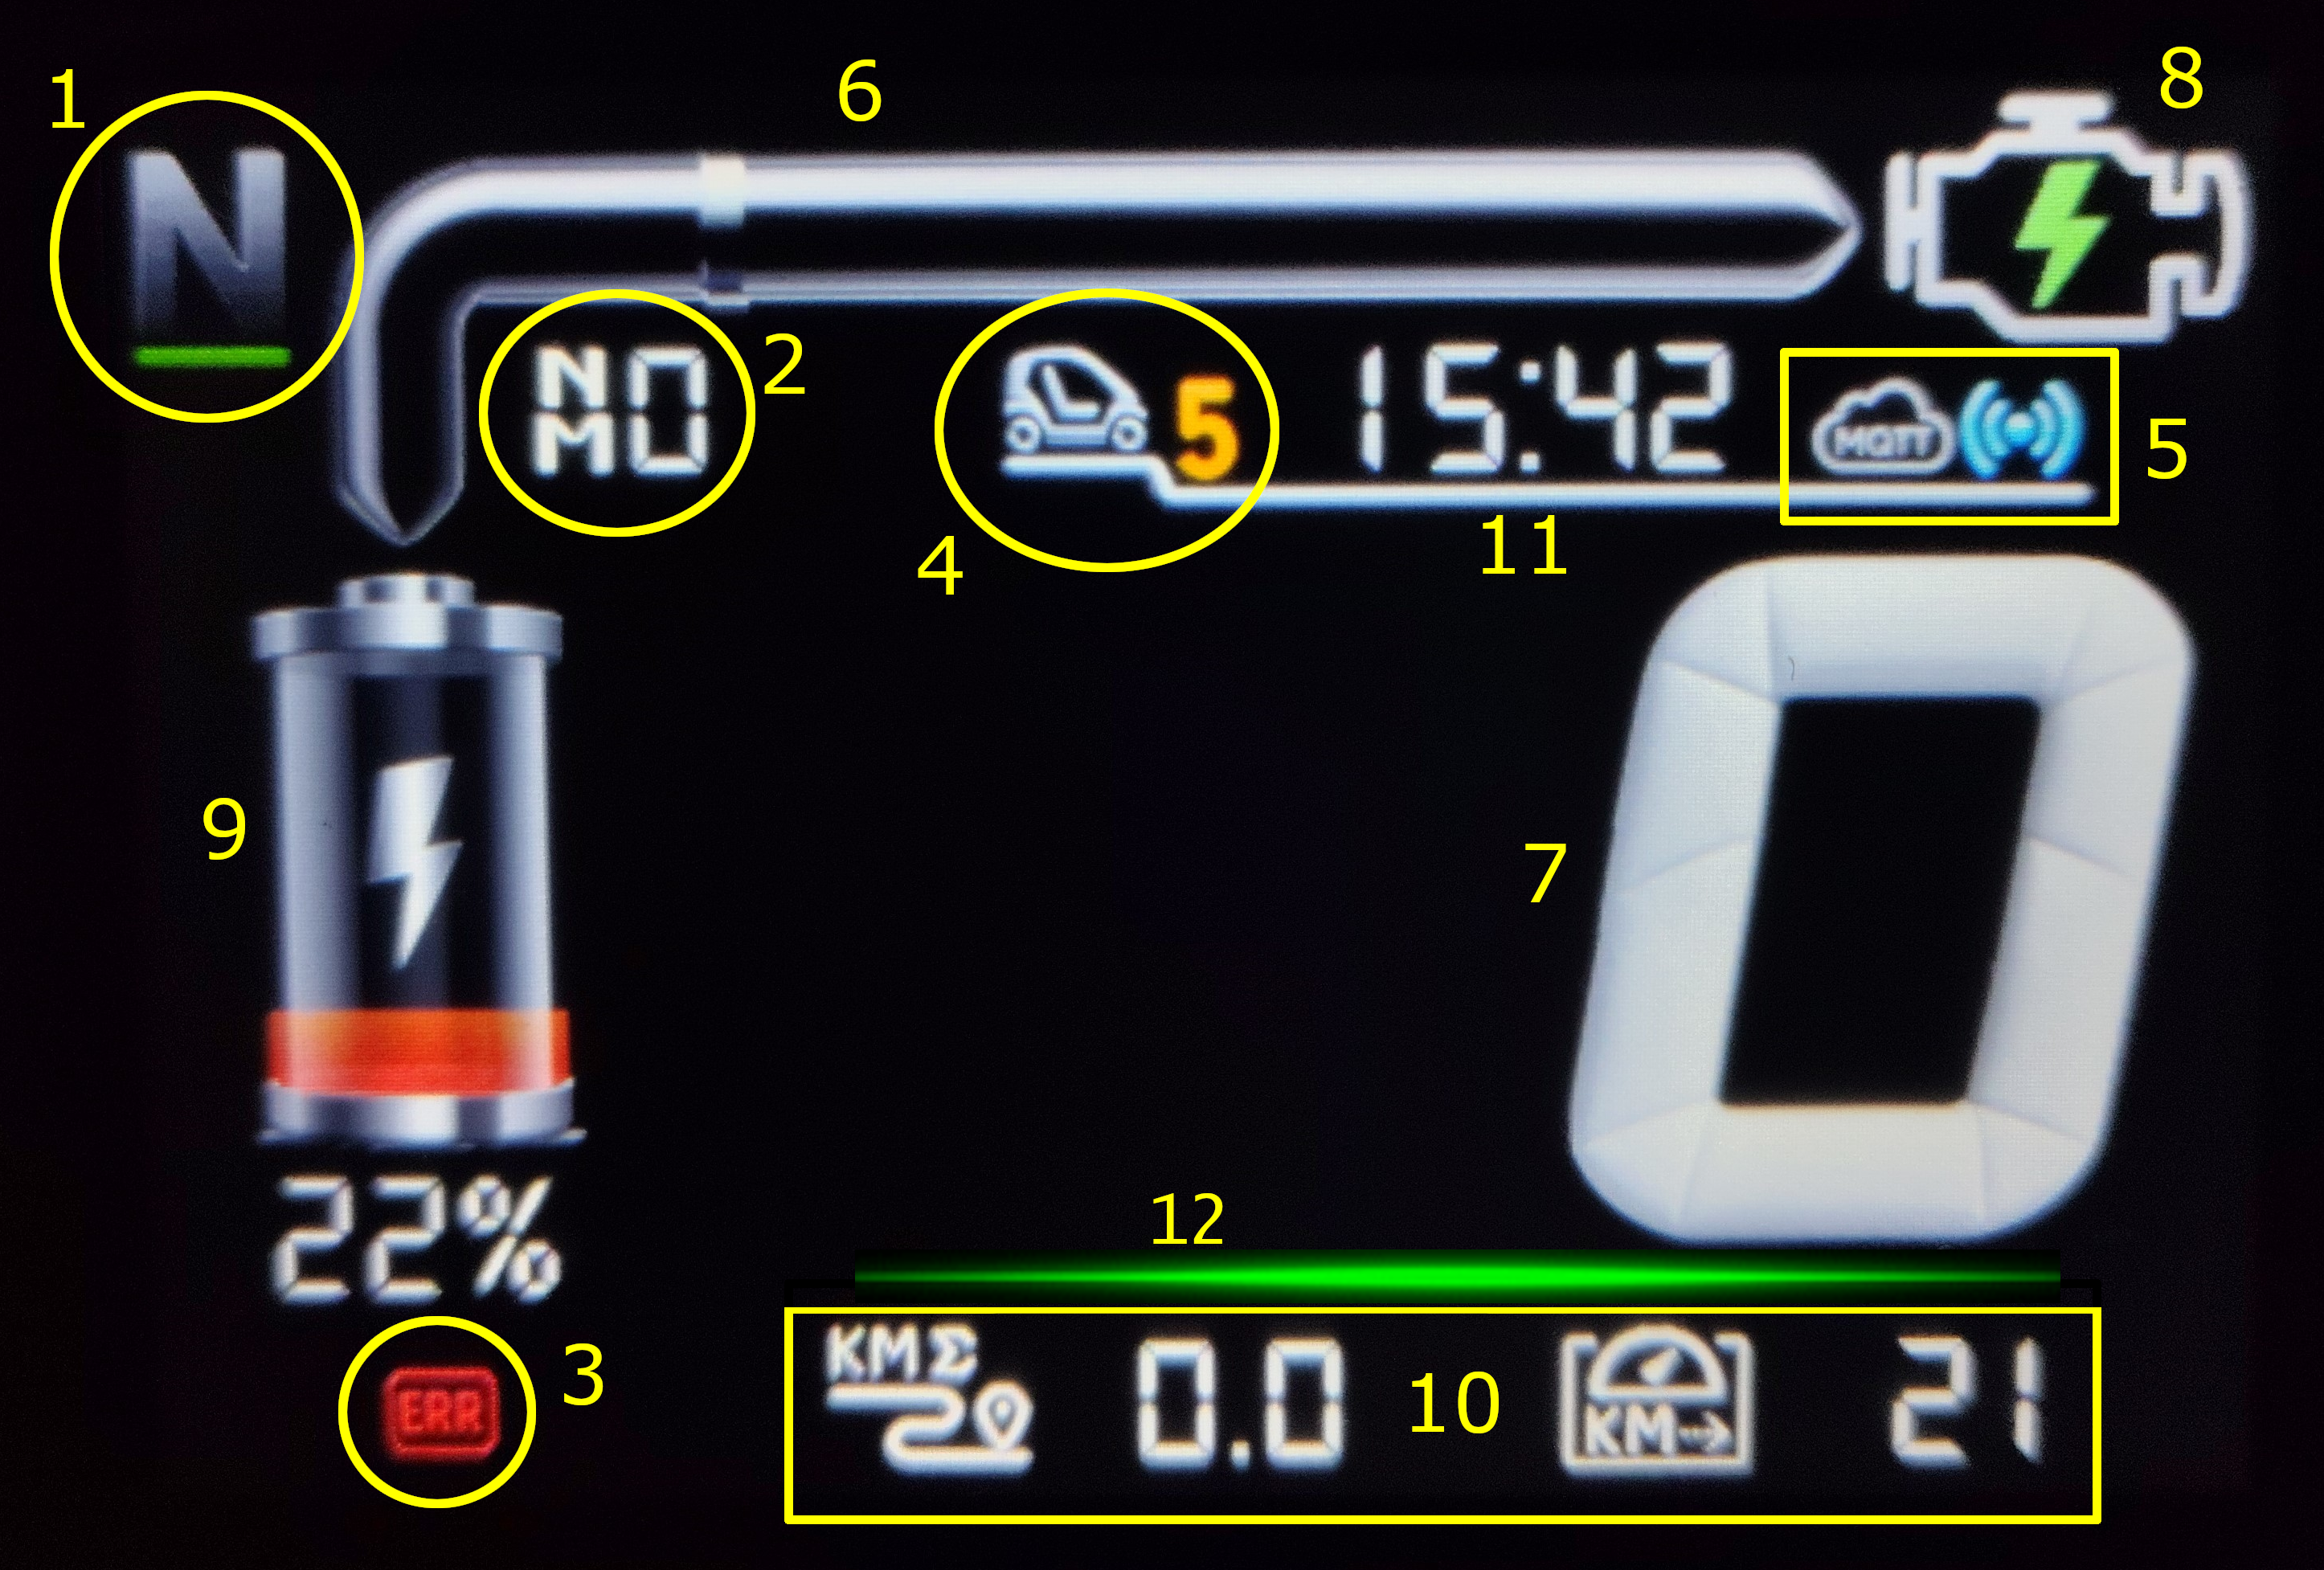
\includegraphics[width=0.8\textwidth]{figures/dashboard_numbers.PNG}
    \caption{Page du tableau de bord avec les parties numérotées.} \label{fig:dashboard_layout}
\end{figure}

\begin{description}
\item[\textbf{1}] Rapport engagé actuel du véhicule, généralement affiché également sur le tableau de bord d'origine.
\item[\textbf{2}] Une valeur choisie entre le couple, la consommation d'énergie et la consommation de courant, qui est utilisée pour remplir la barre de puissance décrite à l'élément 6. Appuyez sur la valeur pour faire défiler les trois options.
\item[\textbf{3}] Icône d'état d'erreur, affichée lorsqu'une erreur est présente.
\item[\textbf{4}] Affiche le trajet actif. Appuyez sur l'icône pour ouvrir la page du trajet.
\item[\textbf{5}] Icônes pour MQTT et Wi-Fi. Grisées en cas de déconnexion, et colorées une fois connecté. Appuyez sur les icônes si vous souhaitez effectuer une nouvelle recherche Wi-Fi ou une reconnexion MQTT.
\item[\textbf{6}] Barre de puissance affichant la valeur sélectionnée à l'élément 2. En partant de la ligne centrale, la barre se remplit de gauche à droite lors de l'accélération, et de droite à gauche lors du freinage régénératif. La barre se remplit avec un dégradé de couleur dans chaque direction, et les \textbf{valeurs maximales et minimales sont personnalisables} sur la page BigToM du serveur web.
\item[\textbf{7}] Affiche la vitesse instantanée du véhicule. Vous pouvez choisir entre km/h et mph dans la page Informations avancées et paramètres du serveur web.
\item[\textbf{8}] Icône moteur, appuyez dessus pour ouvrir la page moteur.
\item[\textbf{9}] Icône colorée avec dégradé de la batterie, appuyez dessus pour ouvrir la page d'informations de la batterie.
\item[\textbf{10}] Valeurs affichées supplémentaires, vous pouvez naviguer entre elles en appuyant sur l'icône pour les modifier.
\item[\textbf{11}] Affiche l'heure et la date, basculez entre elles en appuyant dessus.
\item[\textbf{12}] Limite d'alerte de vitesse personnalisable (verte, jaune ou rouge), voir la Section~\ref{sec:web_btom_tom_sets} pour l'activer.
\end{description}

\section{La disposition des pages}
\label{sec:main-layout}

La disposition peut être divisée en deux parties principales, que nous verrons en détail dans les deux paragraphes suivants. La première est le moniteur de données qui dispose de fonctionnalités pour modifier les données affichées au premier plan en les choisissant parmi celles répertoriées dans la barre latérale. La seconde est la barre d'icônes d'état, généralement située au bas de la page. Les pages batterie, moteur, gyroscope et trajet partagent la même disposition, comme illustré sur l'image.

\begin{figure}[H]
    \centering
    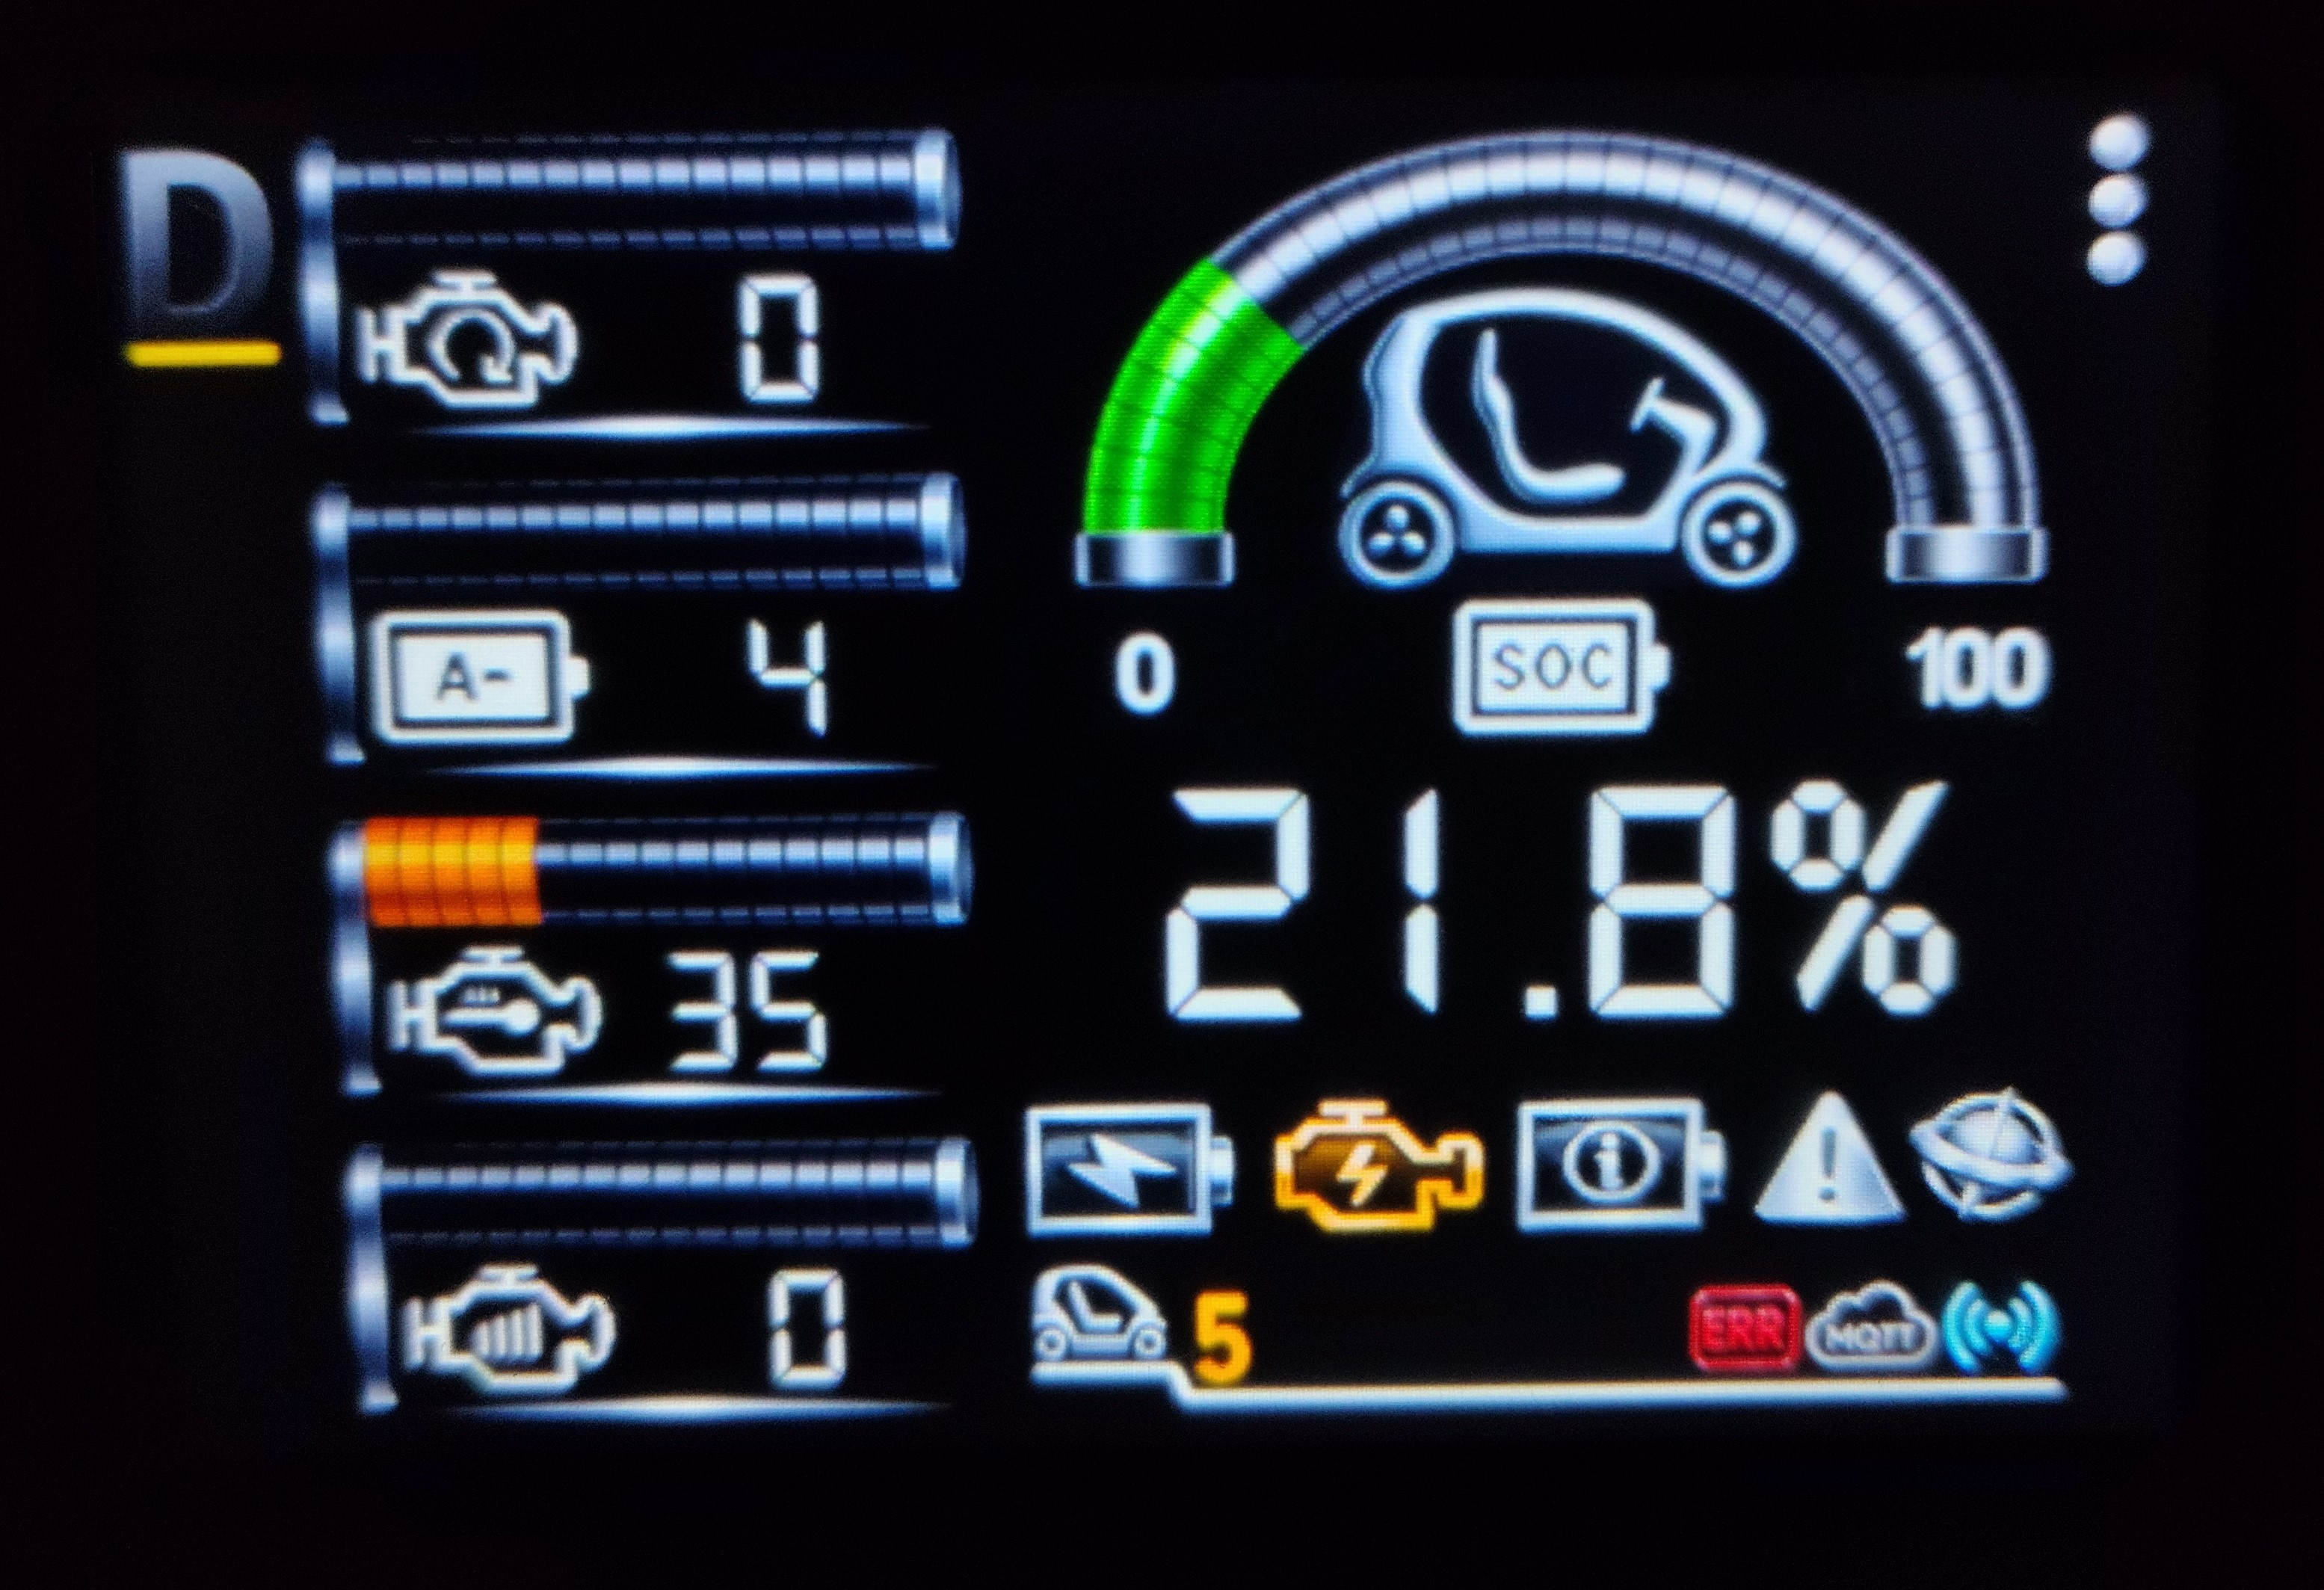
\includegraphics[width=0.8\textwidth]{figures/engine_page.jpg}
    \caption{Exemple de la disposition partagée (la page moteur).}
\end{figure}

Sur le côté gauche de l'écran, comme vous pouvez le voir sur la photo, se trouve une liste de quatre valeurs, regroupées dans une grille minimale. Chaque valeur est associée à son unité de mesure et à une petite icône, unique pour chaque donnée et toutes répertoriées dans la Section~\ref{sec:icon_list}. Au-dessus de la valeur se trouve une barre de progression orange qui représente à quel point la valeur est grande (ou petite) par rapport à sa valeur maximale (ou minimale).\\

La zone droite de l'écran est principalement occupée par la donnée au premier plan (ou simplement la donnée sélectionnée). Elle comporte une grande icône Twizy entourée d'une barre de progression en forme d'arc qui remplit la même fonction que la plus petite abordée précédemment, à la seule différence qu'elle compte 32 étapes au lieu de 16 seulement. Aux extrémités de la barre de progression se trouve la plage ou le multiplicateur de la valeur affichée au centre de la page, qui est celle associée à l'icône affichée juste au-dessus.\\

En bas, se trouve une liste d'icônes utilisées pour basculer entre les différentes pages du ToM+. Les icônes sont les mêmes pour toutes les pages, et elles sont toutes répertoriées dans la Section~\ref{sec:page_icon_list}. Dans le coin supérieur gauche, une petite icône indique le rapport engagé actuel du véhicule. Si vous appuyez dessus, \textbf{elle vous ramènera à la page du tableau de bord} que nous venons d'évoquer. Dans le coin supérieur droit, trois petits points permettent d'ouvrir la page des paramètres lorsqu'on appuie dessus. Enfin, sur la longue ligne blanche en bas de l'écran, se trouve la barre d'état avec quelques icônes que nous aborderons plus tard.

\subsection{Changer la donnée au premier plan}

Modifier la donnée affichée au premier plan est très simple et intuitif. Il vous suffit d'appuyer sur l'icône de la donnée que vous souhaitez afficher au premier plan et les valeurs s'échangeront. De cette façon, vous pouvez également réorganiser les données sur le côté gauche de l'écran, ce qui est très pratique si vous souhaitez avoir une donnée spécifique dans un ordre arbitraire.

\begin{figure}[H]
    \centering
    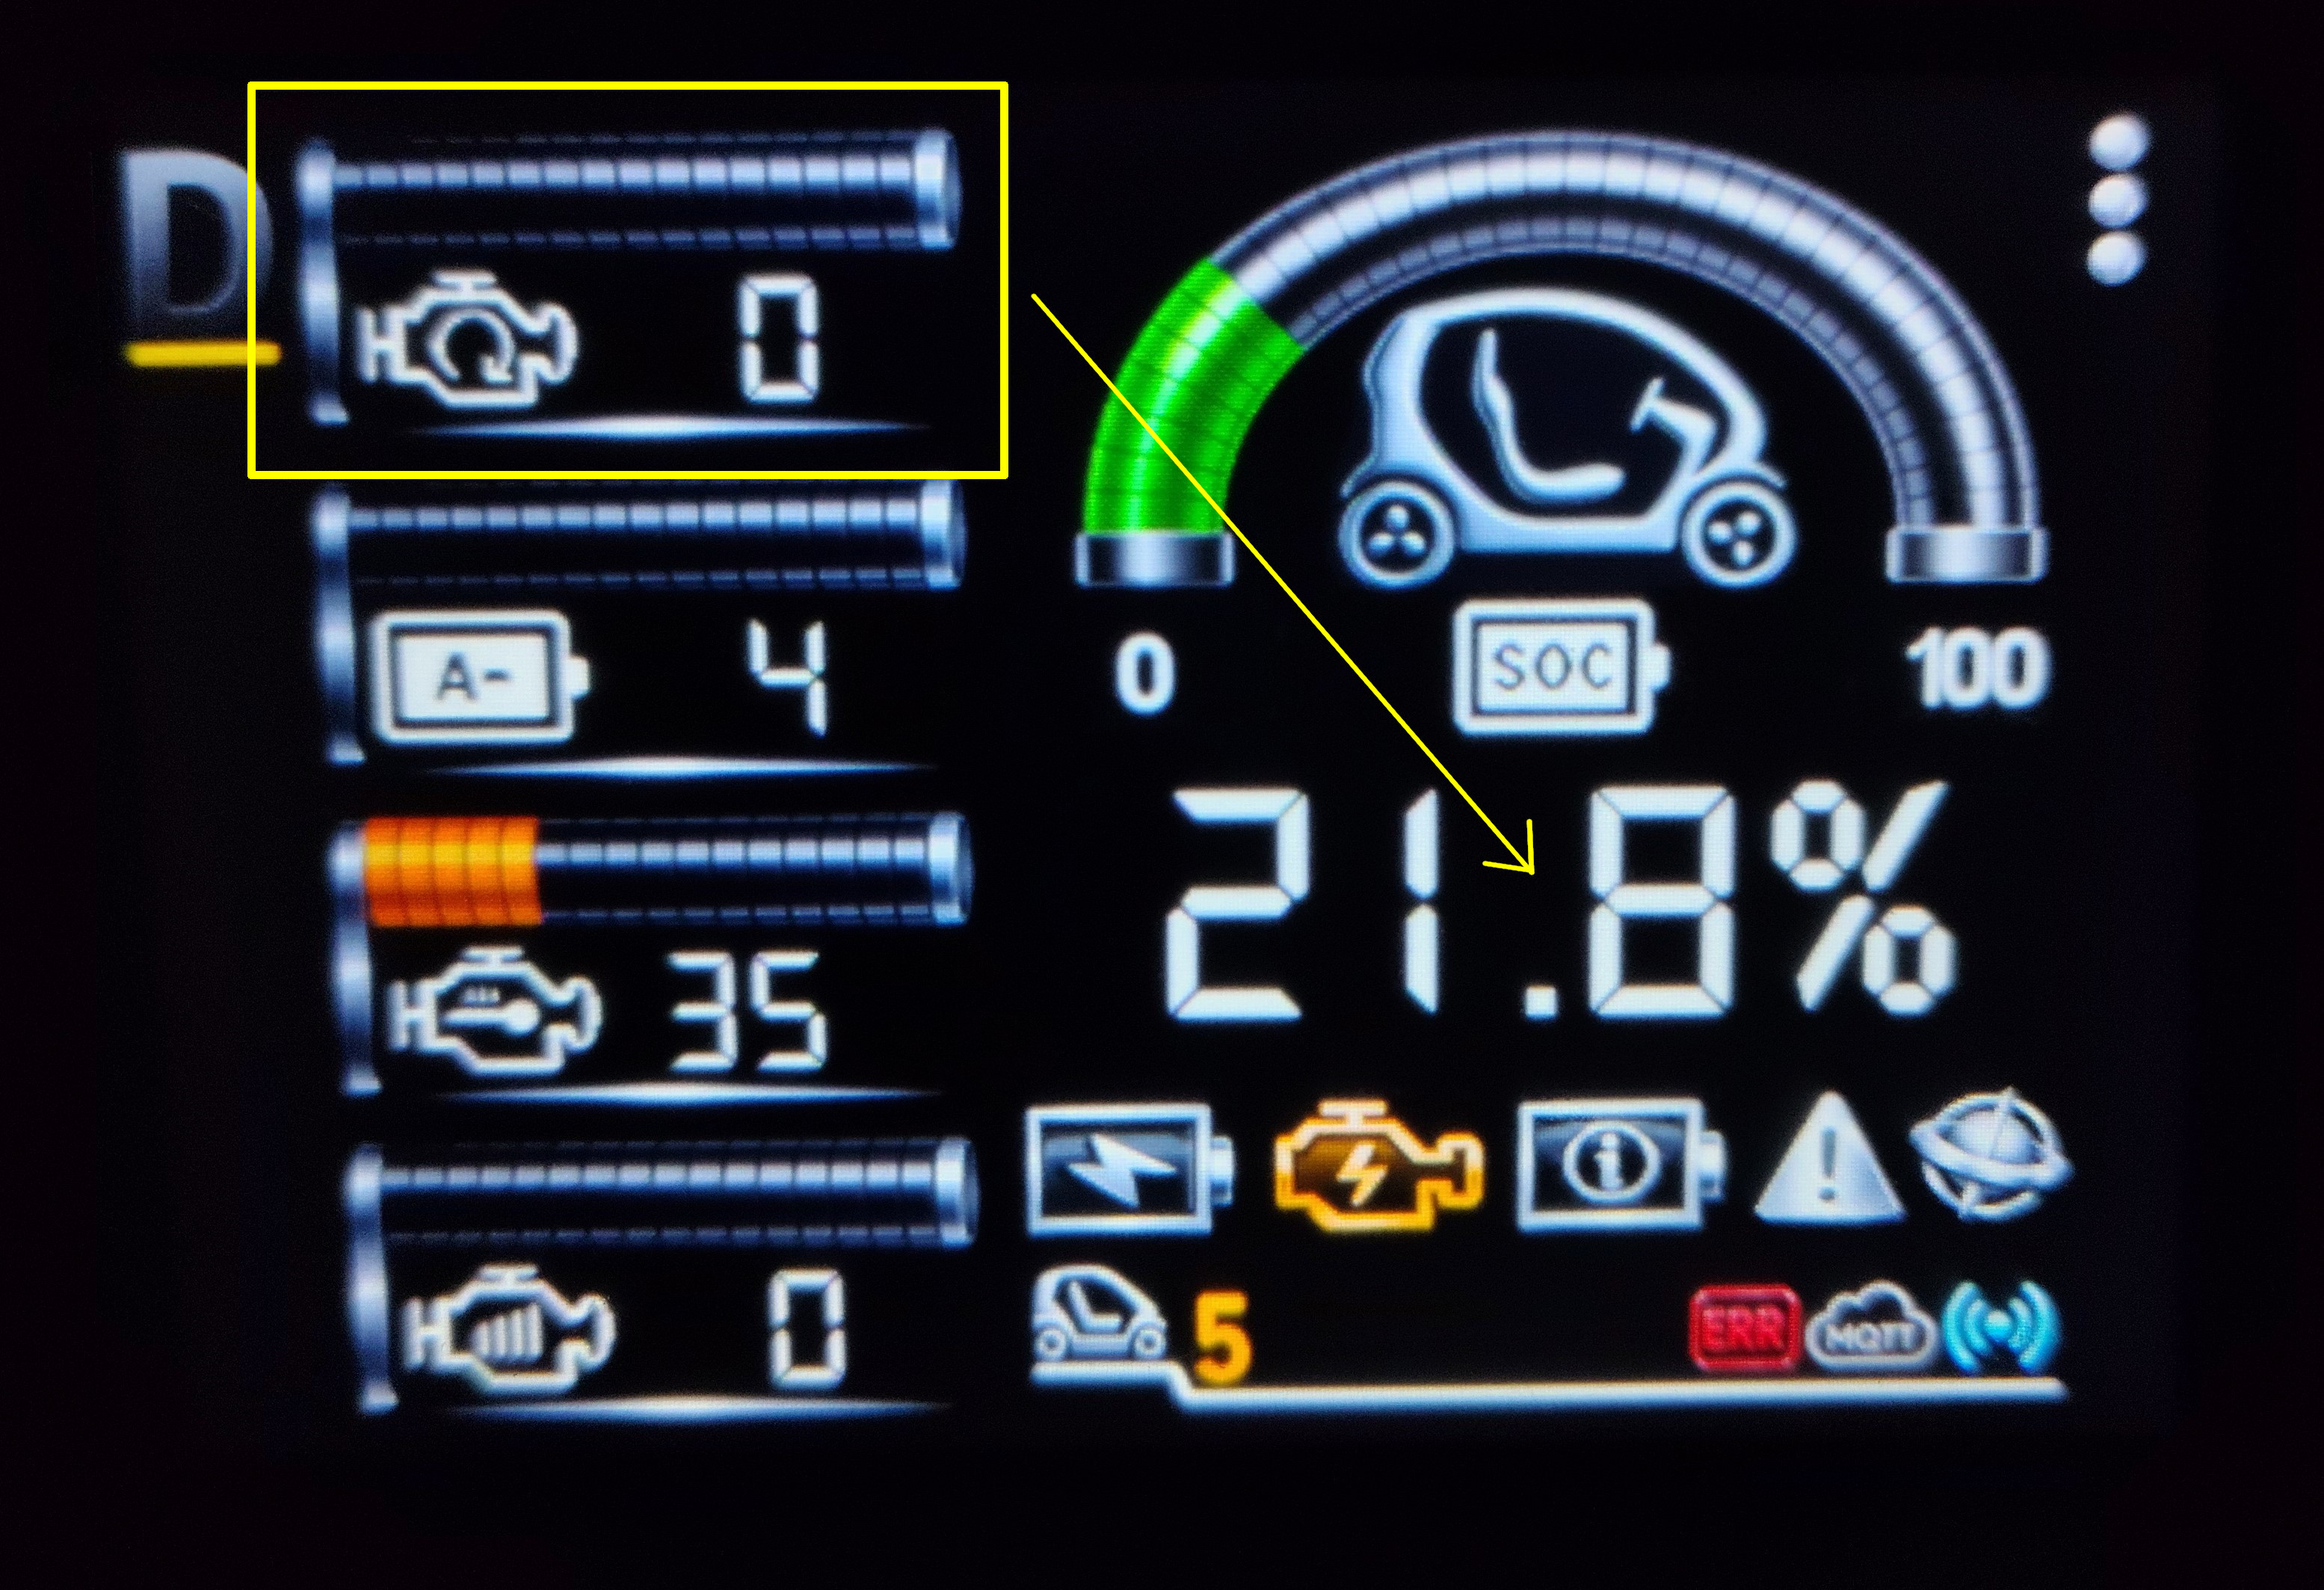
\includegraphics[width=0.7\textwidth]{figures/change_foreground.jpg}
    \caption{Exemple de changement de la donnée au premier plan (sur la page moteur).}
\end{figure}

À titre d'exemple, sur l'image ci-dessus, l'utilisateur a appuyé sur l'icône du régime moteur, qui est actuellement affiché sur le côté gauche de l'écran. Les deux valeurs se sont permutées et le régime moteur est désormais affiché au premier plan, tandis que le SOC de la batterie est affiché dans la grille de gauche.

\subsection{Changer de page active}

Pour changer la page active, vous pouvez appuyer sur l'icône de la page vers laquelle vous souhaitez basculer, située sur la ligne inférieure de l'écran. L'icône deviendra orange et la nouvelle page s'affichera. Dans l'image, la page active est la page moteur.

\begin{figure}[H]
    \centering
    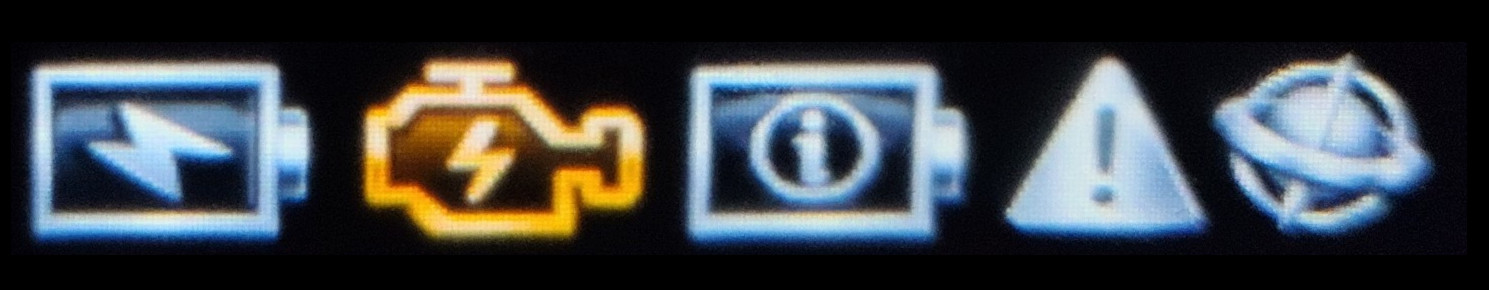
\includegraphics[width=0.7\textwidth]{figures/changing_page.jpg}
    \caption{Exemple de changement de page active (sur la page moteur).}
\end{figure}

Chacune de ces actions peut être effectuée à l'aide du bouton situé sur le commodo d'essuie-glace droit, ce qui est très pratique en conduisant, car vous pouvez garder les yeux sur la route et les mains sur le volant. Le bouton peut être utilisé pour faire défiler les différentes pages, pour modifier la donnée au premier plan et plus encore. Il sera décrit en détail dans la Section~\ref{sec:web_wiper_stalk}.

\subsection{La barre d'icônes d'état}
\label{sec:status_icon_bar}

Sous les boutons de changement de page abordés au paragraphe précédent, se trouve une longue ligne blanche qui vous indique l'état de la connexion réseau ainsi que le déclenchement des alarmes ou des erreurs. Au début de la ligne, comme vous pouvez le voir sur l'image, se trouve une petite icône twizy avec un numéro : c'est un bouton qui vous mènera à la page du trajet, qui sera abordée plus tard dans la Section~\ref{sec:trip_page}. Voyons maintenant la barre d'icônes d'état.

\begin{figure}[H]
    \centering
    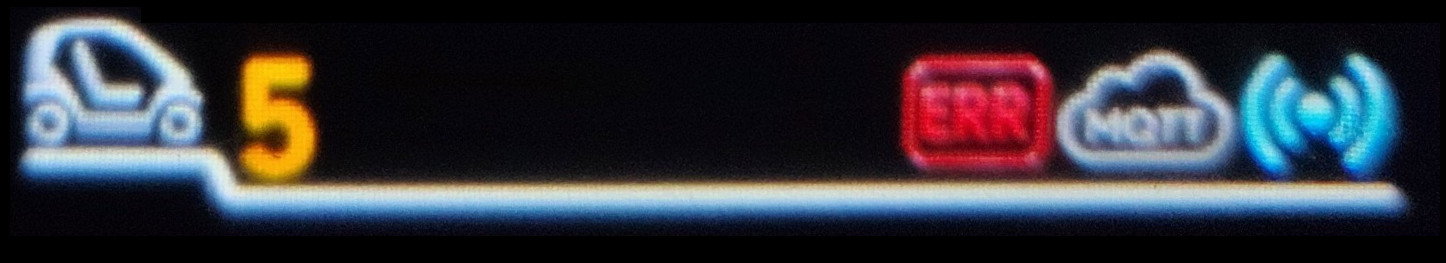
\includegraphics[width=0.7\textwidth]{figures/status_icon_bar.jpg}
    \caption{La barre d'icônes d'état.}
\end{figure}

En partant du côté droit de l'image, vous verrez un symbole d'onde bleu magnétique qui représente l'état de la connexion \textbf{Wi-Fi}. En effet, s'il est allumé et fixe comme ci-dessus, cela signifie que ToM est connecté à un réseau Wi-Fi, qu'il s'agisse d'un réseau public ou d'un réseau de la liste que vous avez définie. Lorsque l'icône est grisée, ToM n'est connecté à aucun réseau et recherchera à nouveau des réseaux Wi-Fi après une période de recharge de cinq minutes. Vous pouvez également forcer un nouveau balayage dès que possible en appuyant sur l'icône. Enfin, si l'icône clignote, ToM a effectué une recherche Wi-Fi, a trouvé un ou plusieurs réseaux et tente de se connecter à l'un d'eux.\\

L'icône suivante est un nuage violet contenant le texte \textbf{« MQTT »} et, comme vous pouvez le deviner, elle représente l'état de la connexion \textbf{MQTT}. La position de cette icône est fixe et ne peut pas être modifiée, tout comme celle du Wi-Fi. Une autre similitude avec l'icône précédente est qu'elle peut être soit fixe, soit grisée avec le même code couleur que précédemment.\\

Ensuite, nous avons l'icône d'erreur, qui est un rectangle rouge contenant le texte \textbf{« ERR »}. Elle s'affichera lorsqu'une erreur est présente ou sera masquée lorsqu'il n'y a pas d'erreur.\\

Enfin, nous avons les icônes d'alarme, représentées par des étoiles colorées. Les étoiles disponibles sont celles présentées sur l'image ; vous pouvez sélectionner celle à utiliser pour chaque alarme sur la page Déclencheurs d'alarme du serveur web. Vous pouvez y choisir de les faire clignoter ou non.

\begin{figure}[H]
    \centering
    
\includegraphics[width=0.7\textwidth]{figures/alarm_icons.png}
    \caption{Les icônes d'alarme.}
    \label{fig:alarm_icons}
\end{figure}

\subsection{Fenêtres surgissantes (Pop-ups)}

Sur ces pages, des fenêtres surgissantes apparaîtront en fonction de vos configurations définies sur la page « Déclencheurs d'alarme » du serveur web. Il existe deux types principaux de pop-ups : le premier ne disparaîtra pas tant que vous ne l'aurez pas remarqué et appuyé dessus (ce type bloquera l'ensemble du système, mettant en pause les valeurs de la grille de gauche ainsi que la valeur au premier plan). Sinon, si vous ne souhaitez pas être dérangé en conduisant, vous pouvez utiliser le second type de pop-up, spécialement conçu pour disparaître automatiquement après 10 secondes.\\

Vous pouvez voir ici un exemple du type de pop-up le plus simple où l'icône d'avertissement entourée continuera de clignoter. Comme vous pouvez le constater, elle est composée d'un encadré jaune avec un contour pointillé qui contient l'icône de la valeur et la valeur elle-même qui a déclenché l'alarme préalablement définie sur la page du serveur web (température du moteur = 35\textdegree~C).

\begin{figure}[H]
    \centering
    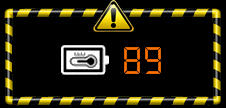
\includegraphics[width=0.7\textwidth]{figures/pop-up.PNG}
    \caption{Un exemple de fenêtre surgissante (pop-up).}
\end{figure}

\section{La page d'informations sur la batterie}

La page d'informations sur la batterie vous fournira des informations plus détaillées sur chaque cellule de la batterie. Comme vous le savez peut-être, les batteries standards de la Twizy possèdent 14 cellules et un capteur de température partagé pour chaque paire de cellules. Sur cette page, vous pouvez surveiller la tension de chaque cellule ainsi que sa température, et avoir une vue d'ensemble de la tension totale de la batterie. L'image montre son apparence habituelle.

\begin{figure}[H]
    \centering
    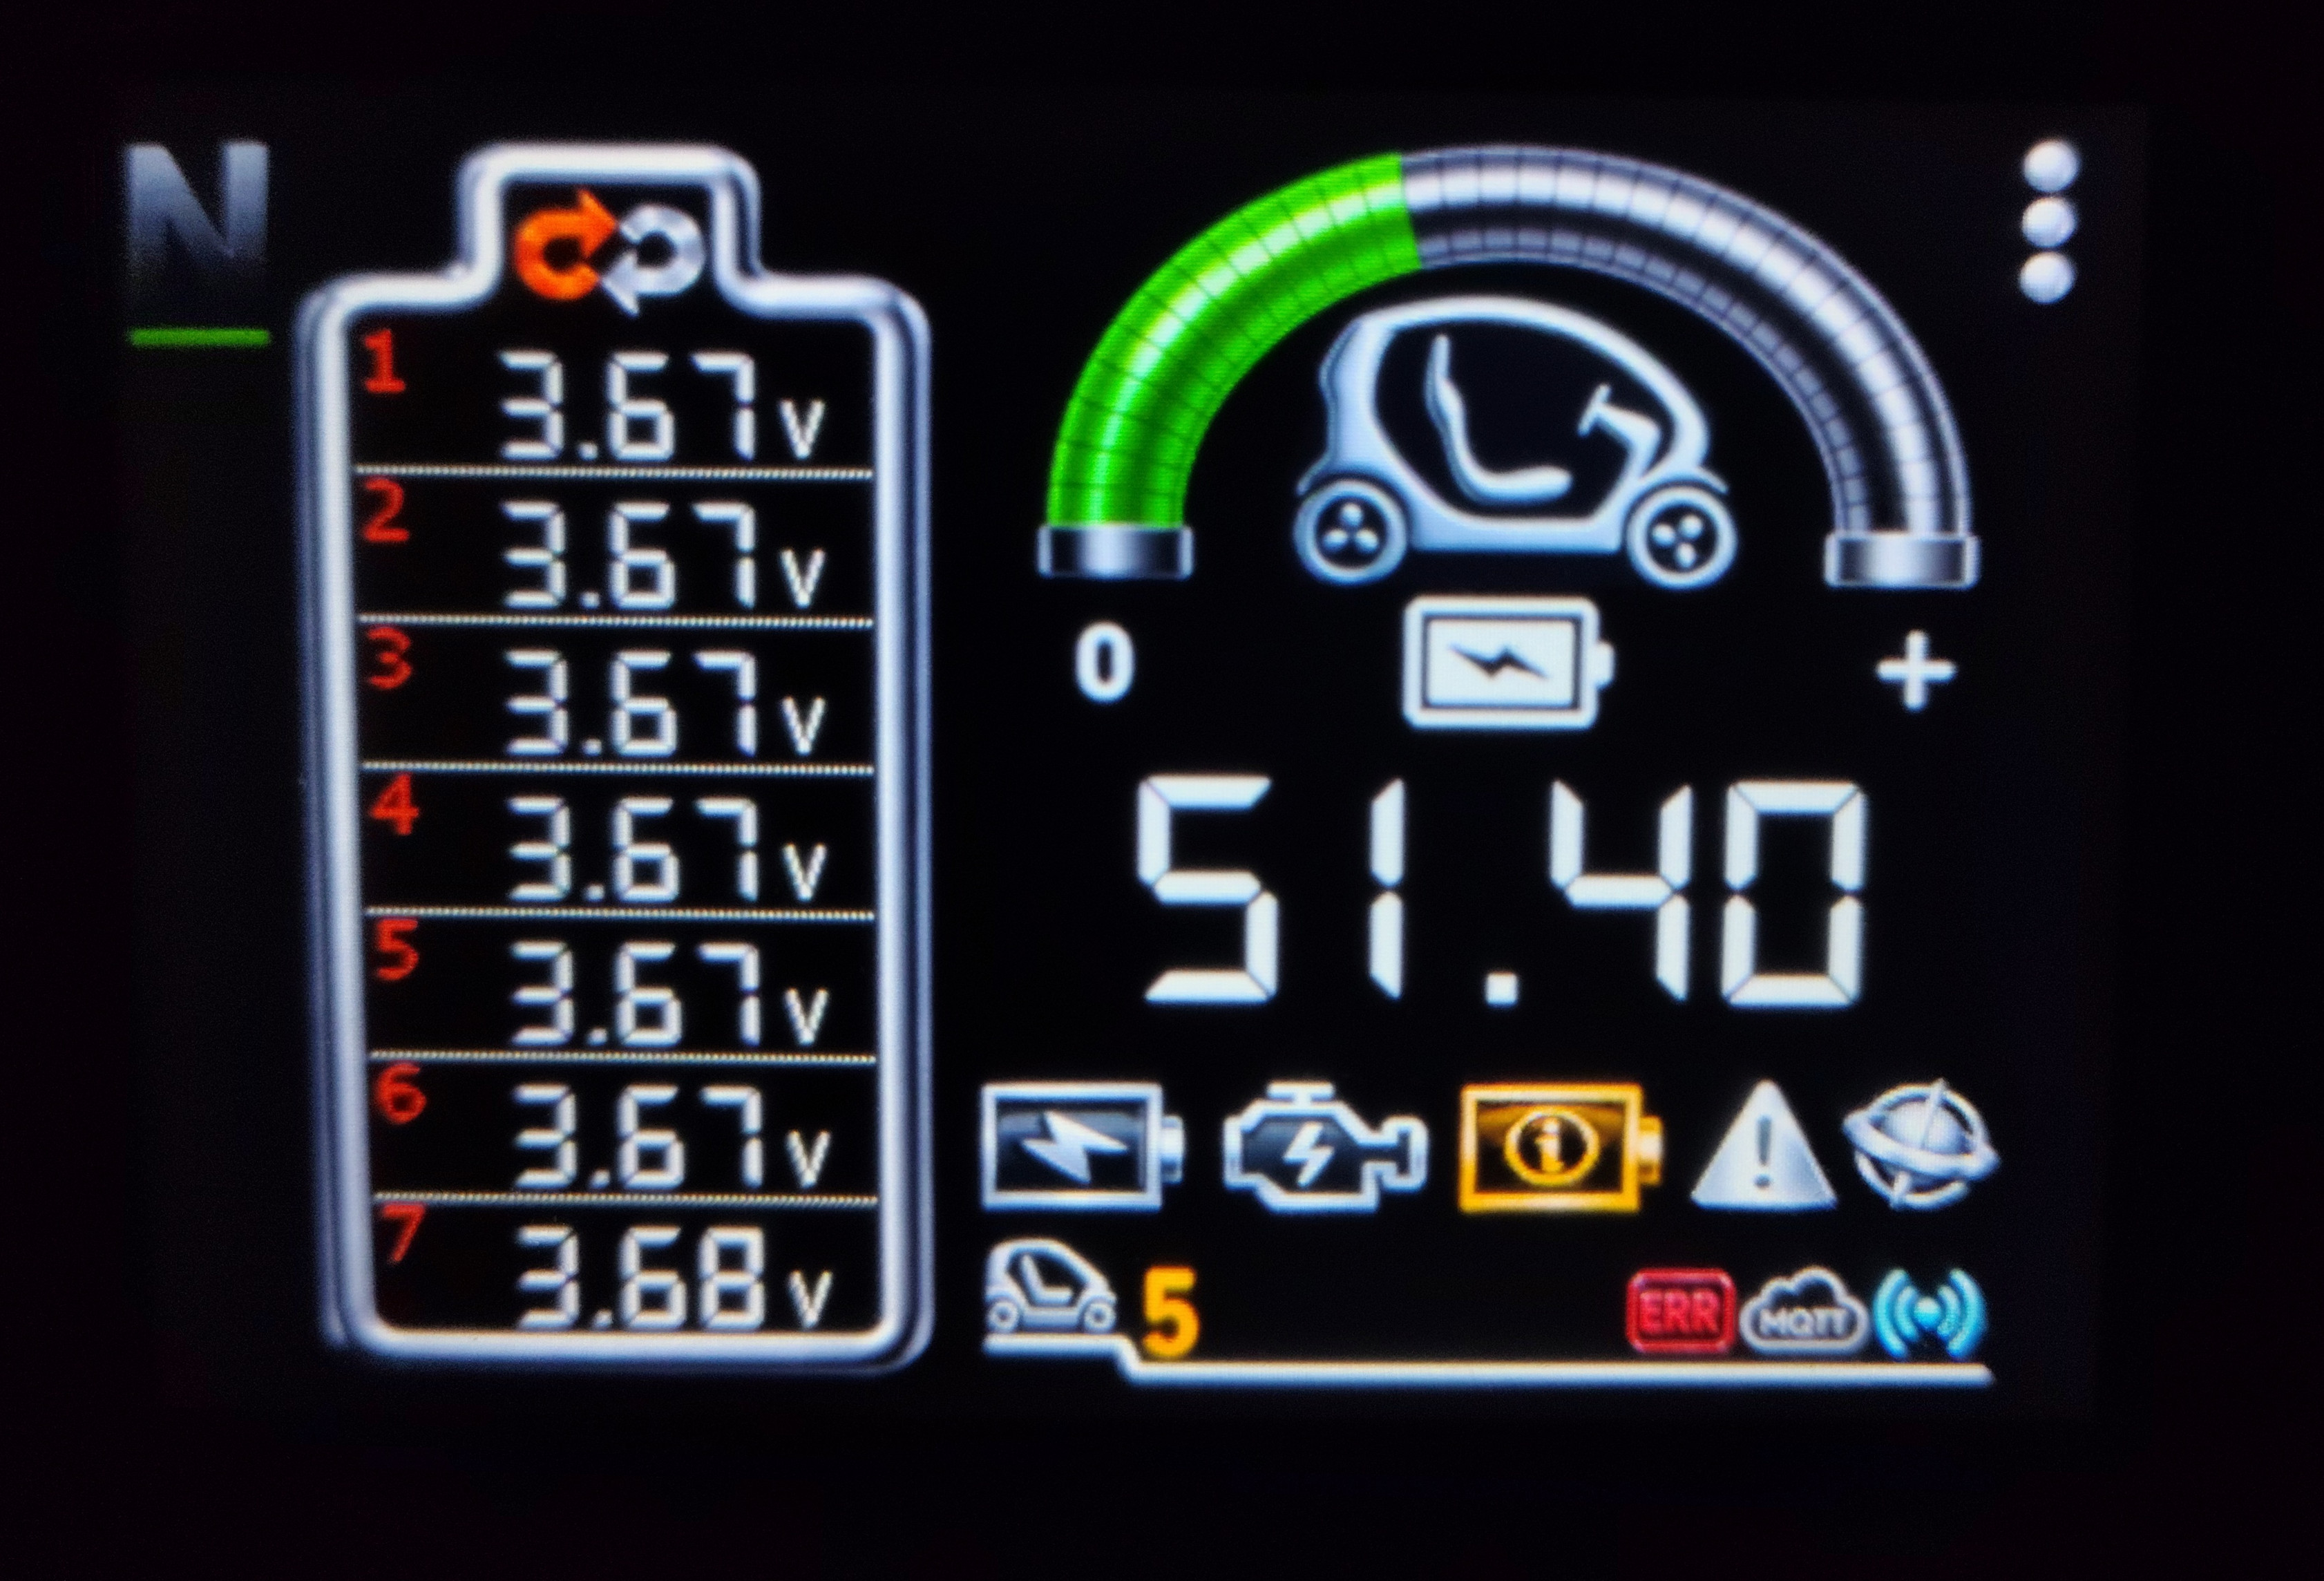
\includegraphics[width=0.8\textwidth]{figures/binfo_page.jpg}
    \caption{La page d'informations sur la batterie.}
\end{figure}

\subsection{Vérification de la tension et de la température}

Comme indiqué sur l'image ci-dessus, sur le côté gauche de la page se trouve une ligne blanche en forme de batterie qui contient un petit tableau avec les tensions des sept premières cellules. Pour voir les tensions des cellules restantes, appuyez sur le symbole de flèche orange et blanche (celui entouré sur la photo suivante) et la grille affichera les valeurs suivantes.

Si vous appuyez à nouveau sur ce même bouton fléché, les données affichées changeront à nouveau pour devenir les températures des cellules, exprimées en degrés Celsius. La valeur au premier plan changera également, et comme vous pouvez le remarquer d'après l'icône située au-dessus, elle affiche la température totale de la batterie, qui est identique à celle de chaque cellule dans cet exemple. Reportez-vous à l'image ci-dessous pour voir la modification.

\begin{figure}[ht]
    \centering

    \begin{subfigure}[t]{0.48\textwidth}
        \centering
        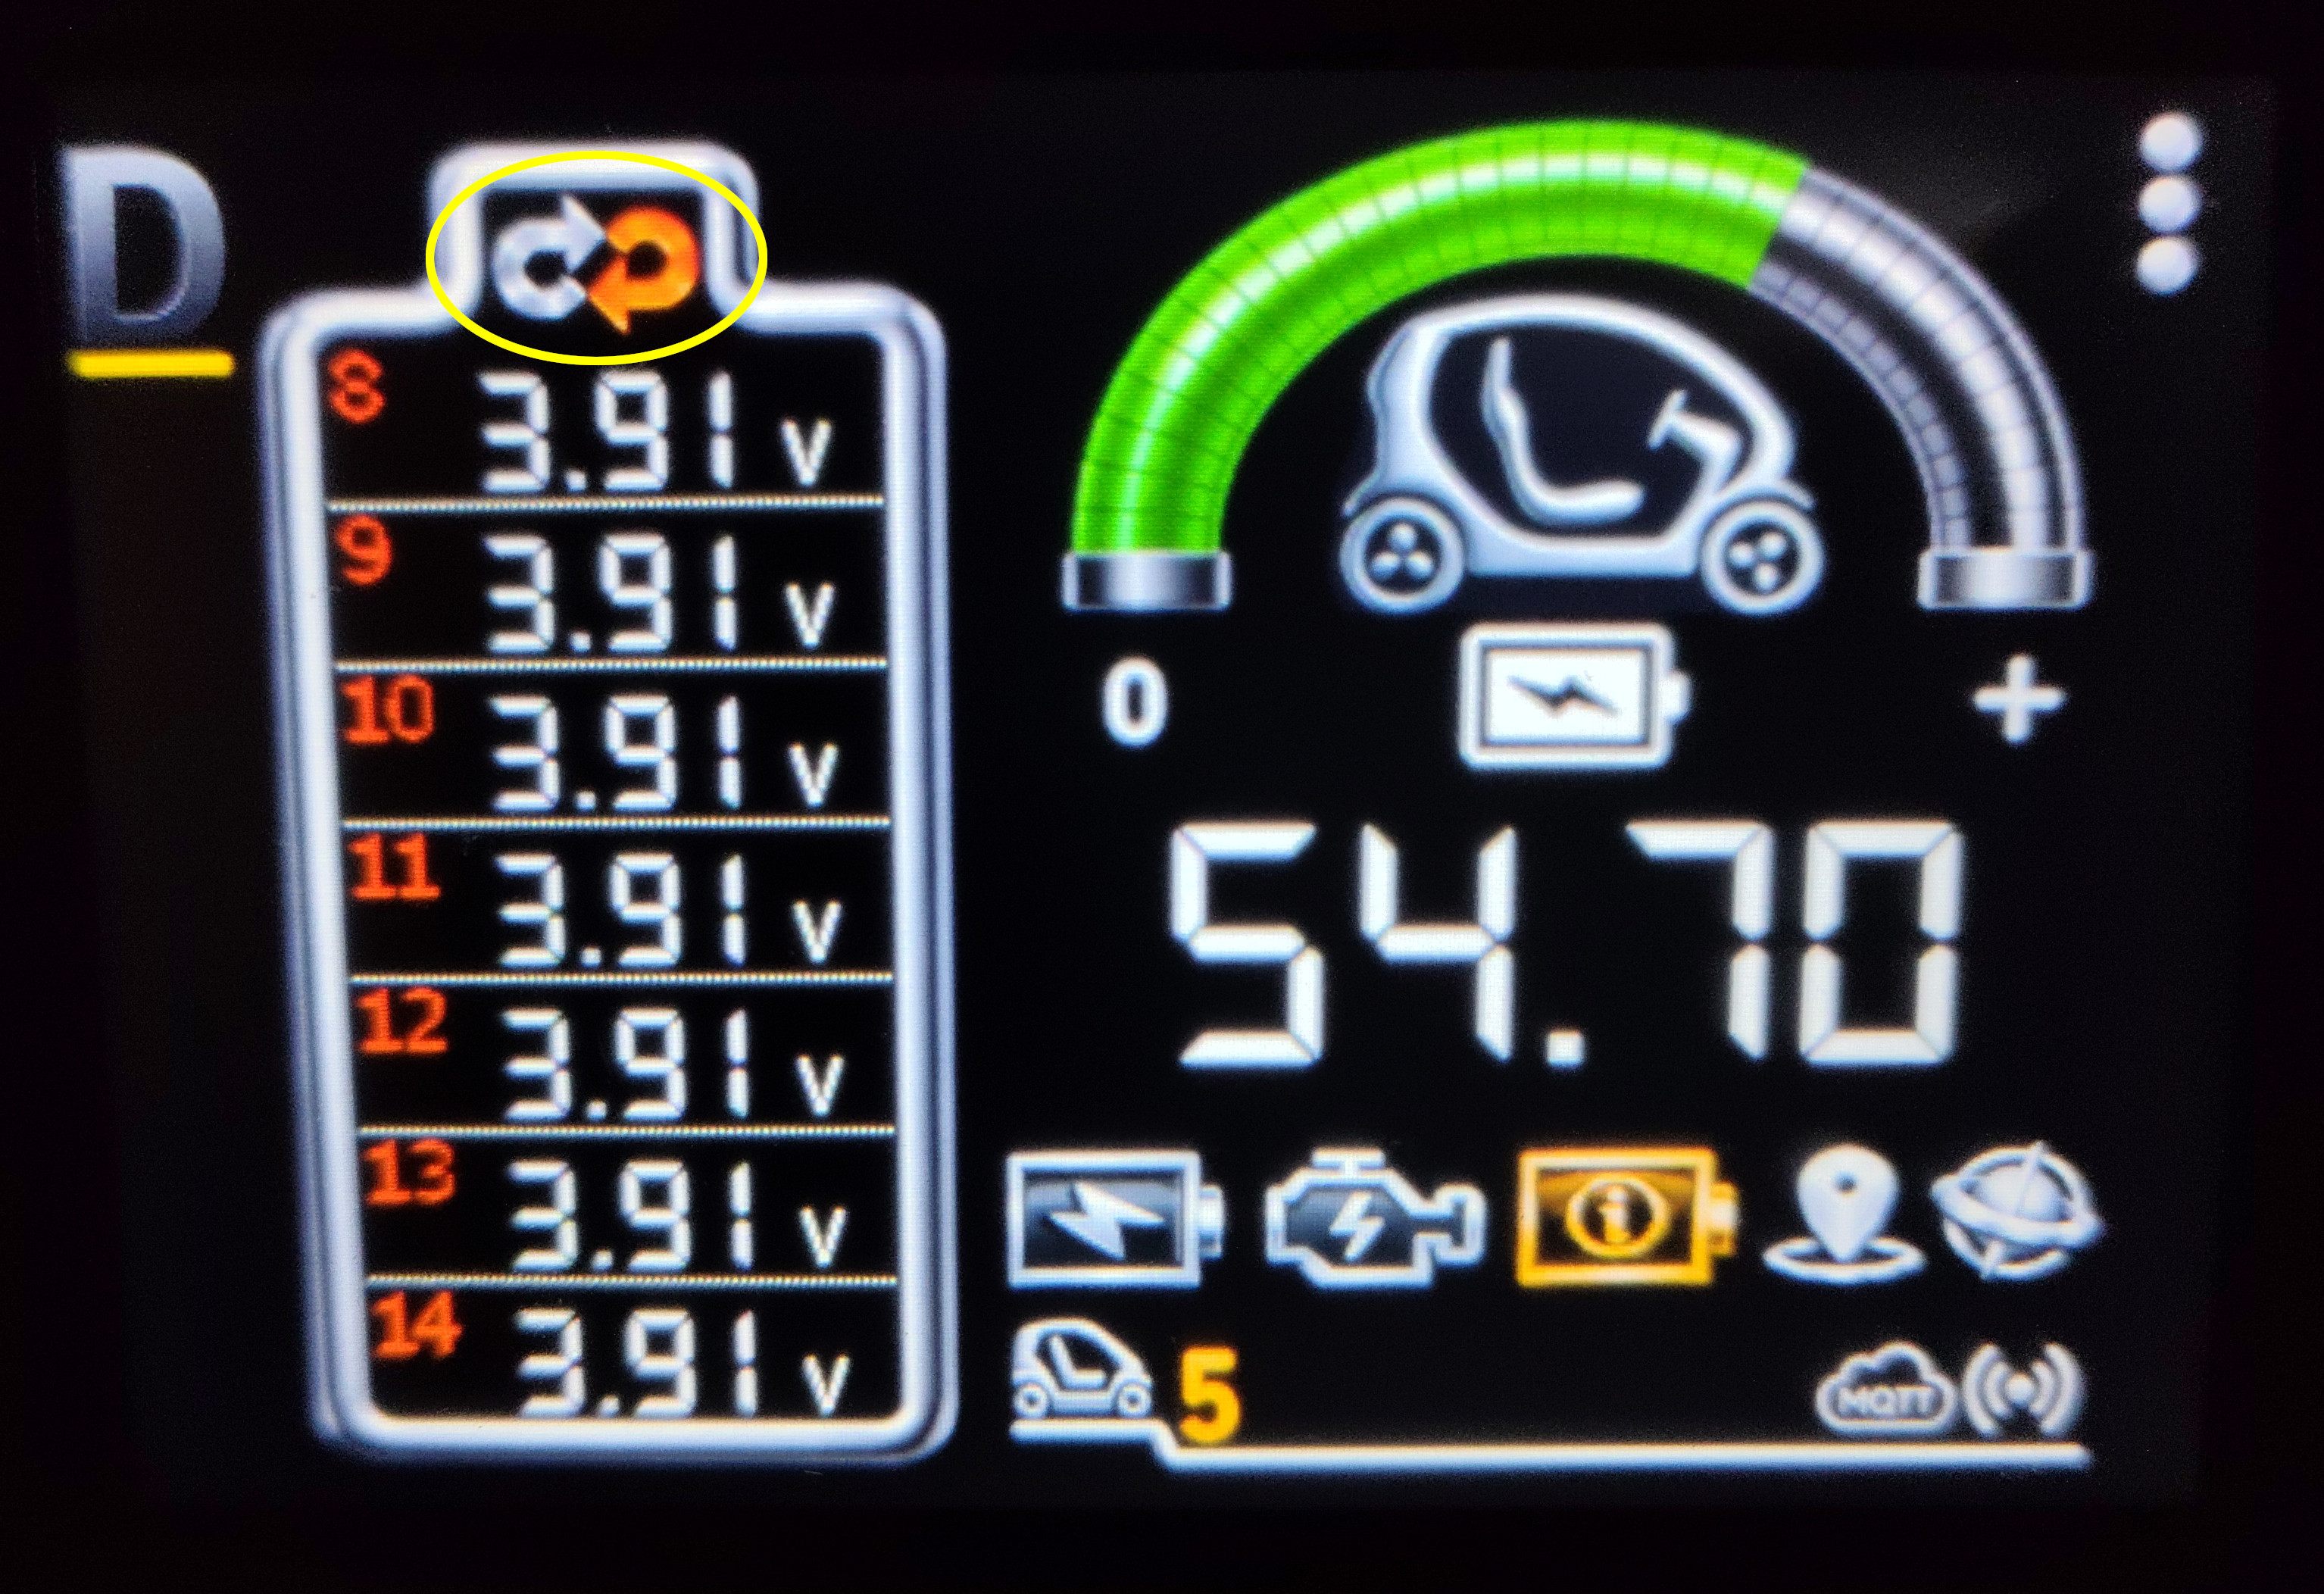
\includegraphics[width=\linewidth]{figures/binfo_page2.jpg}
        \caption{Tensions des cellules restantes.}
    \end{subfigure}
    \hfill
    \begin{subfigure}[t]{0.48\textwidth}
        \centering
        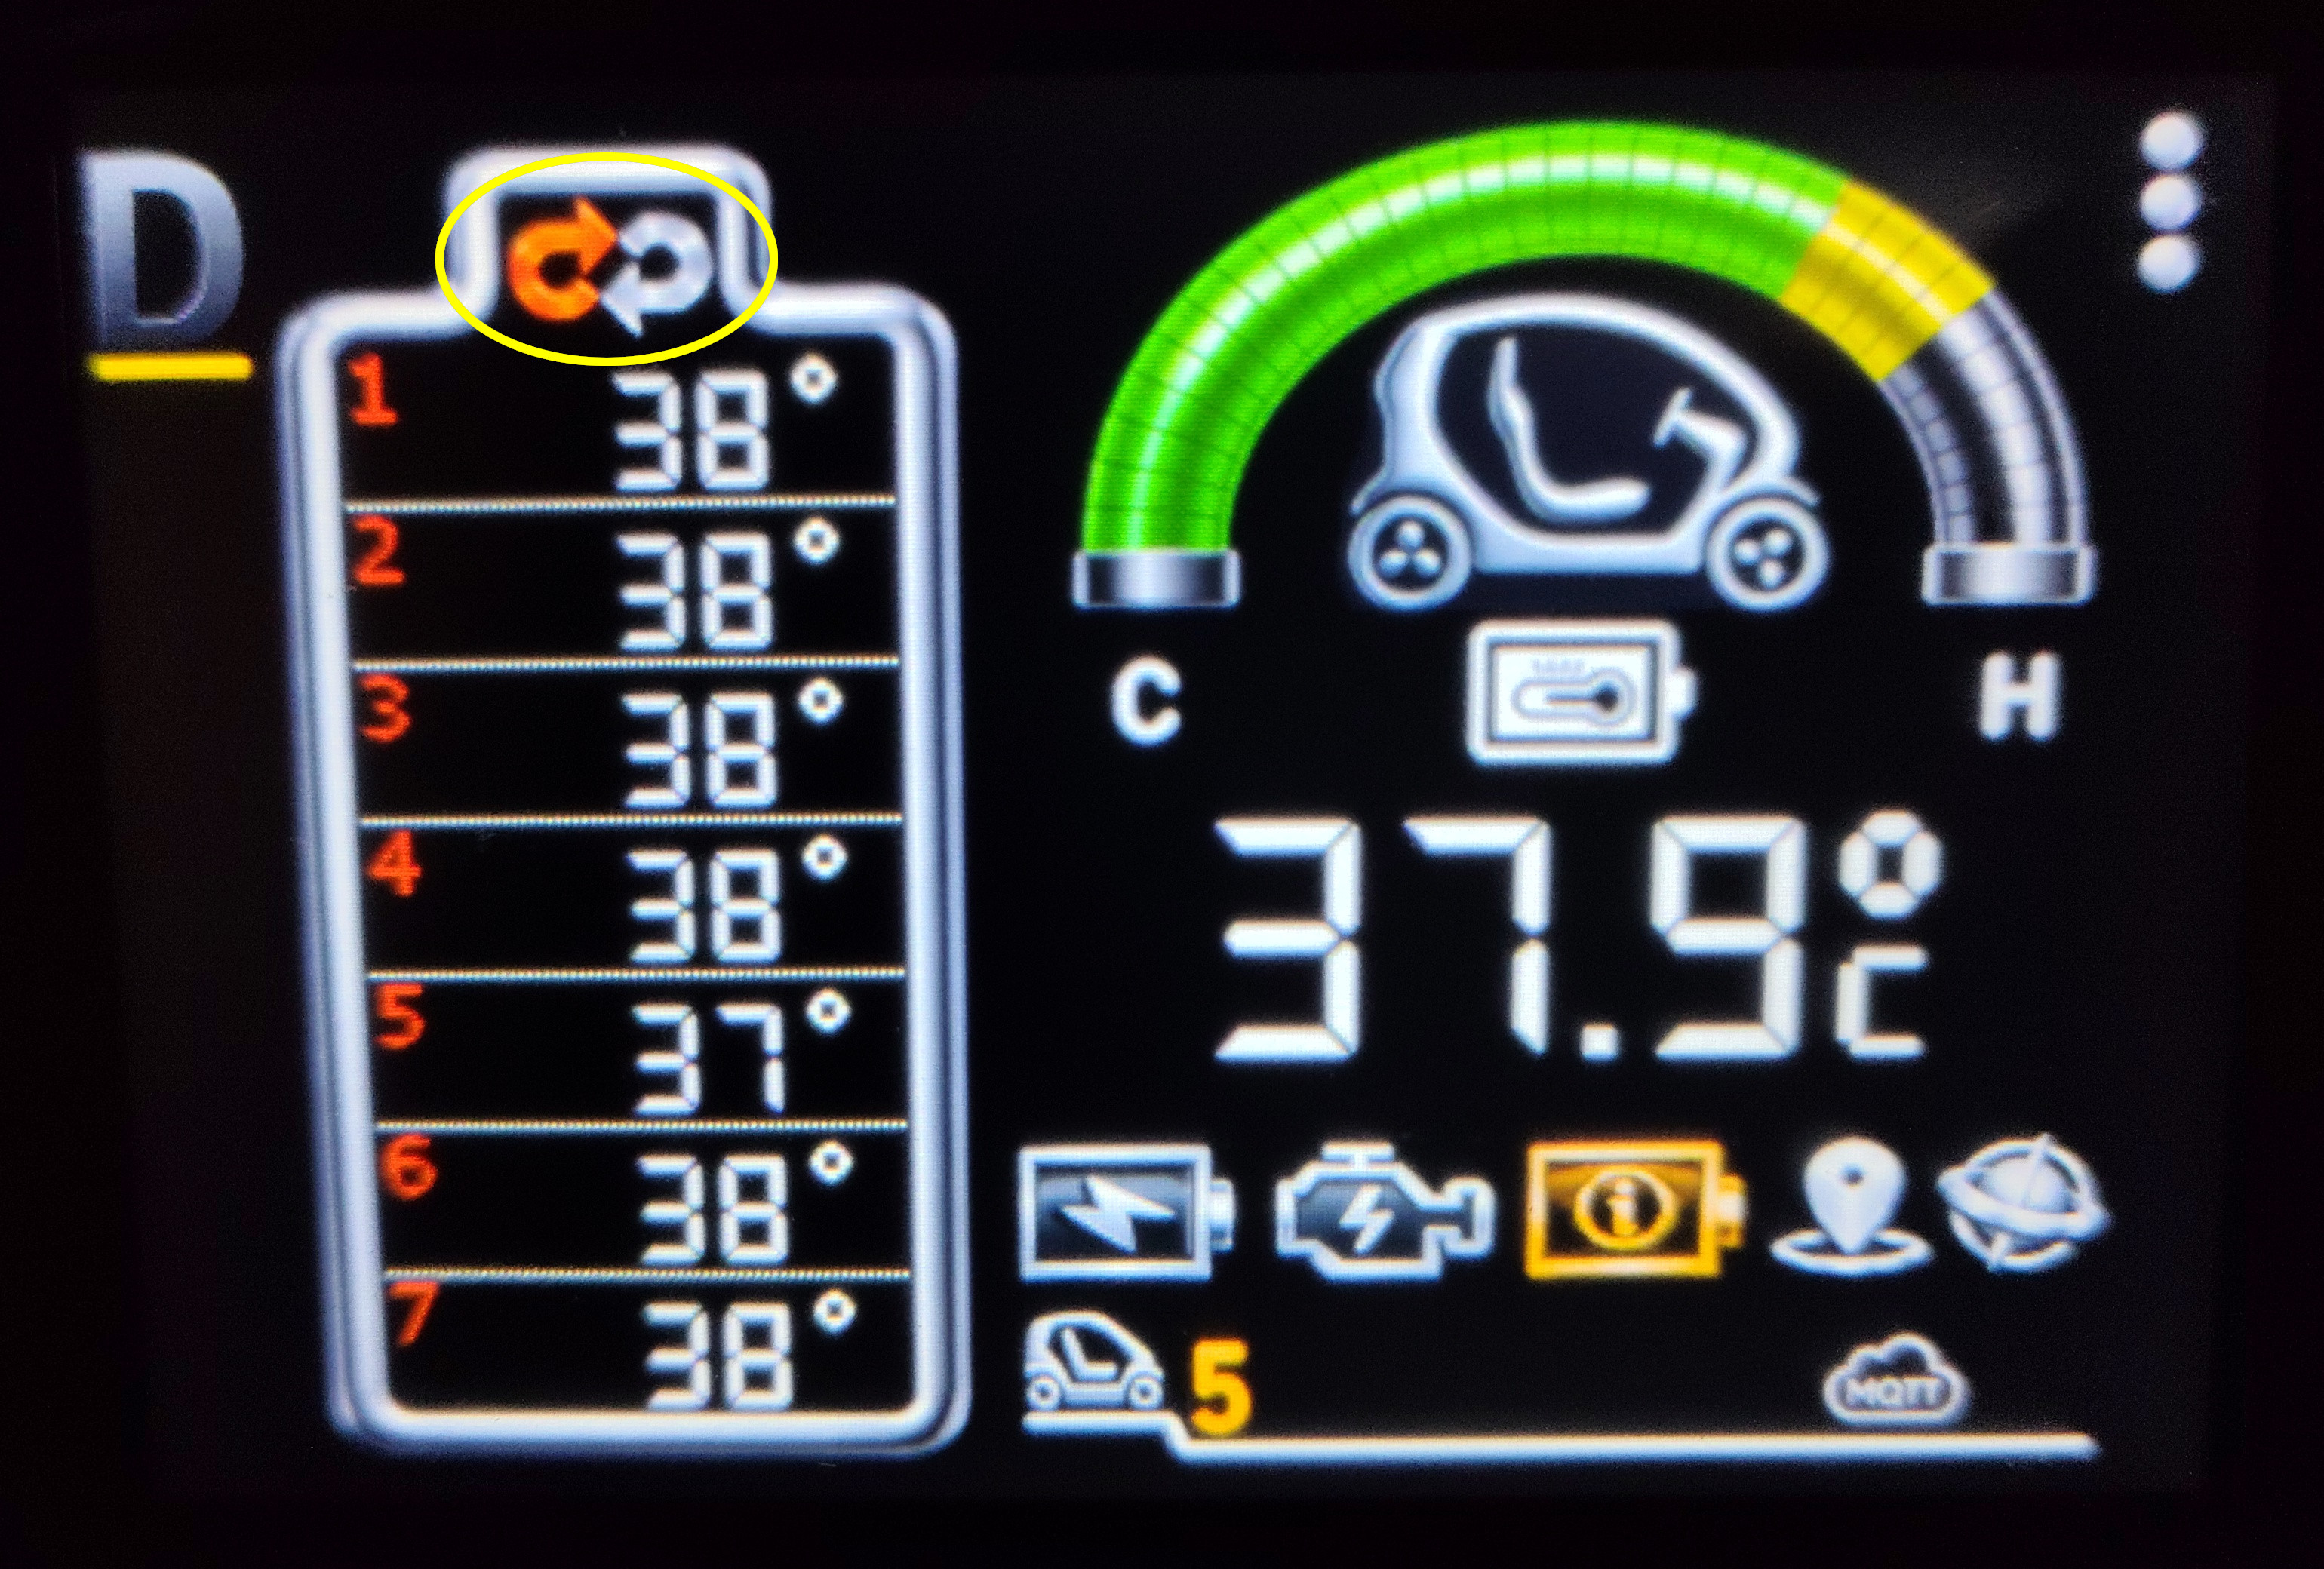
\includegraphics[width=\linewidth]{figures/binfo_page3.jpg}
        \caption{Températures des cellules.}
    \end{subfigure}
\end{figure}

\subsection{La page d'informations condensées de la batterie}
\label{sec:condensed_binfo}

En appuyant à nouveau sur le même bouton, vous accéderez à une page spéciale qui contient toutes les données abordées dans le paragraphe précédent en une seule fois.

\begin{figure}[H]
    \centering
    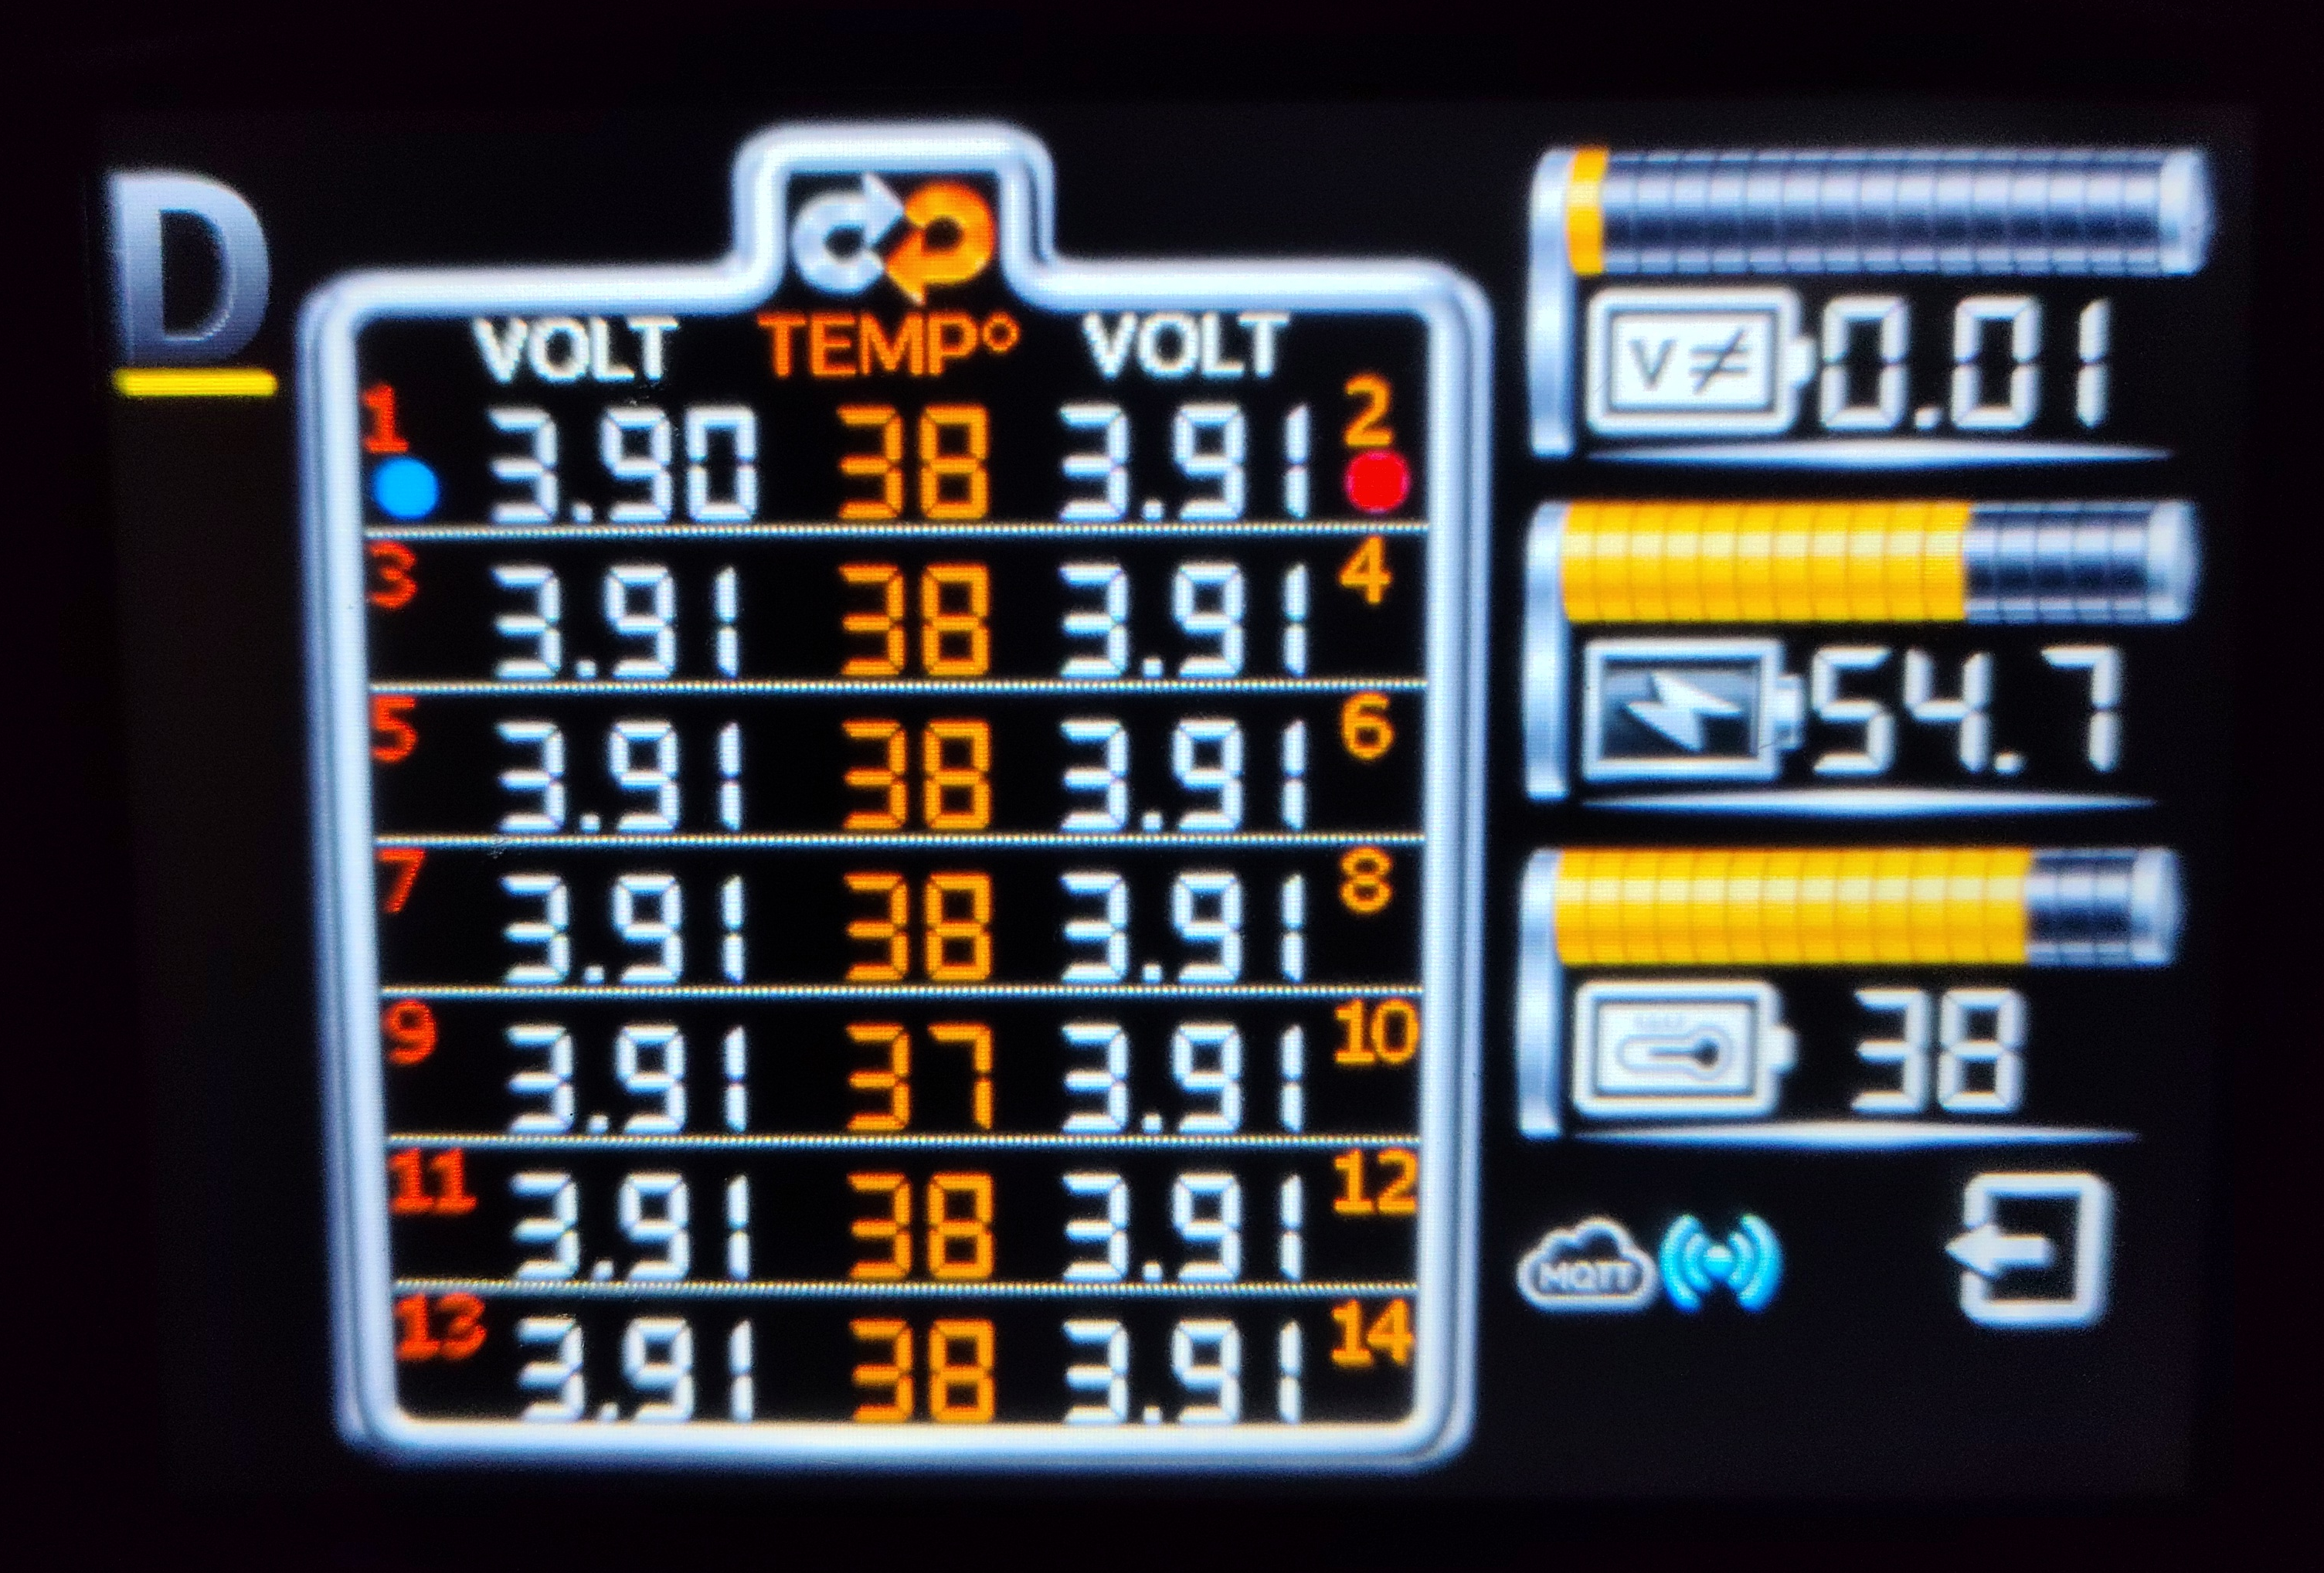
\includegraphics[width=0.8\textwidth]{figures/binfo_page_condensed.png}
    \caption{La page d'informations condensées de la batterie.}
\end{figure}

Sur la photo ci-dessus, vous verrez que l'écran est divisé en deux parties. La première est la même ligne blanche en forme de batterie, mais un peu plus grande, afin de contenir toutes les valeurs de tension et de température. La température est située entre les deux cellules qui partagent ce capteur de température. Sur le côté droit de la page, vous pouvez voir la valeur qui était auparavant affichée au premier plan, c'est-à-dire la tension totale de la batterie et la température totale de la batterie. Il y a également la valeur du SOC en première position car elle est toujours utile.\\

Sur cette page, il n'y avait pas assez d'espace pour placer les boutons de changement de page, car il est plus important d'avoir les icônes d'état dont nous avons parlé précédemment. Si vous devez changer de page, vous pouvez appuyer sur le bouton de sortie dans le coin inférieur droit, puis vous serez redirigé vers une page contenant les commandes permettant de modifier la page active.\\

Une note importante de la dernière mise à jour concerne la différence entre la cellule ayant la tension minimale et celle ayant la tension maximale, respectivement représentées par un point bleu et un point rouge. Cette valeur est très importante car elle peut vous indiquer si la batterie est en bonne santé ou non. Si la différence est trop élevée, cela signifie que la batterie est déséquilibrée et cela pourrait être le signe d'un problème. ToM+ vous affichera cette valeur dans la page d'informations condensées de la batterie, et vous pouvez également définir un déclencheur d'alarme sur le serveur web pour être averti lorsque la différence est trop élevée.\\

Vous pouvez décider dans les paramètres si cette page condensée de la batterie est affichée comme page par défaut lorsque vous appuyez sur le bouton d'informations de la batterie ou non. Le processus est illustré dans la Section~\ref{sec:settings_page}. Si vous sélectionnez l'option permettant d'avoir les quatre pages vues dans ce paragraphe, vous pouvez également appuyer sur le bouton fléché sur la page condensée pour revenir aux autres pages d'informations de la batterie.

\section{La page du journal des alarmes}
\label{sec:alarm_log}

Sur cette page, vous pourrez consulter tous les déclenchements d'alarmes, au cas où vous en auriez manqué un ou si vous les avez mis en sourdine pour ne pas être dérangé en conduisant. Voyons à quoi elle ressemble.

\begin{figure}[H]
    \centering
    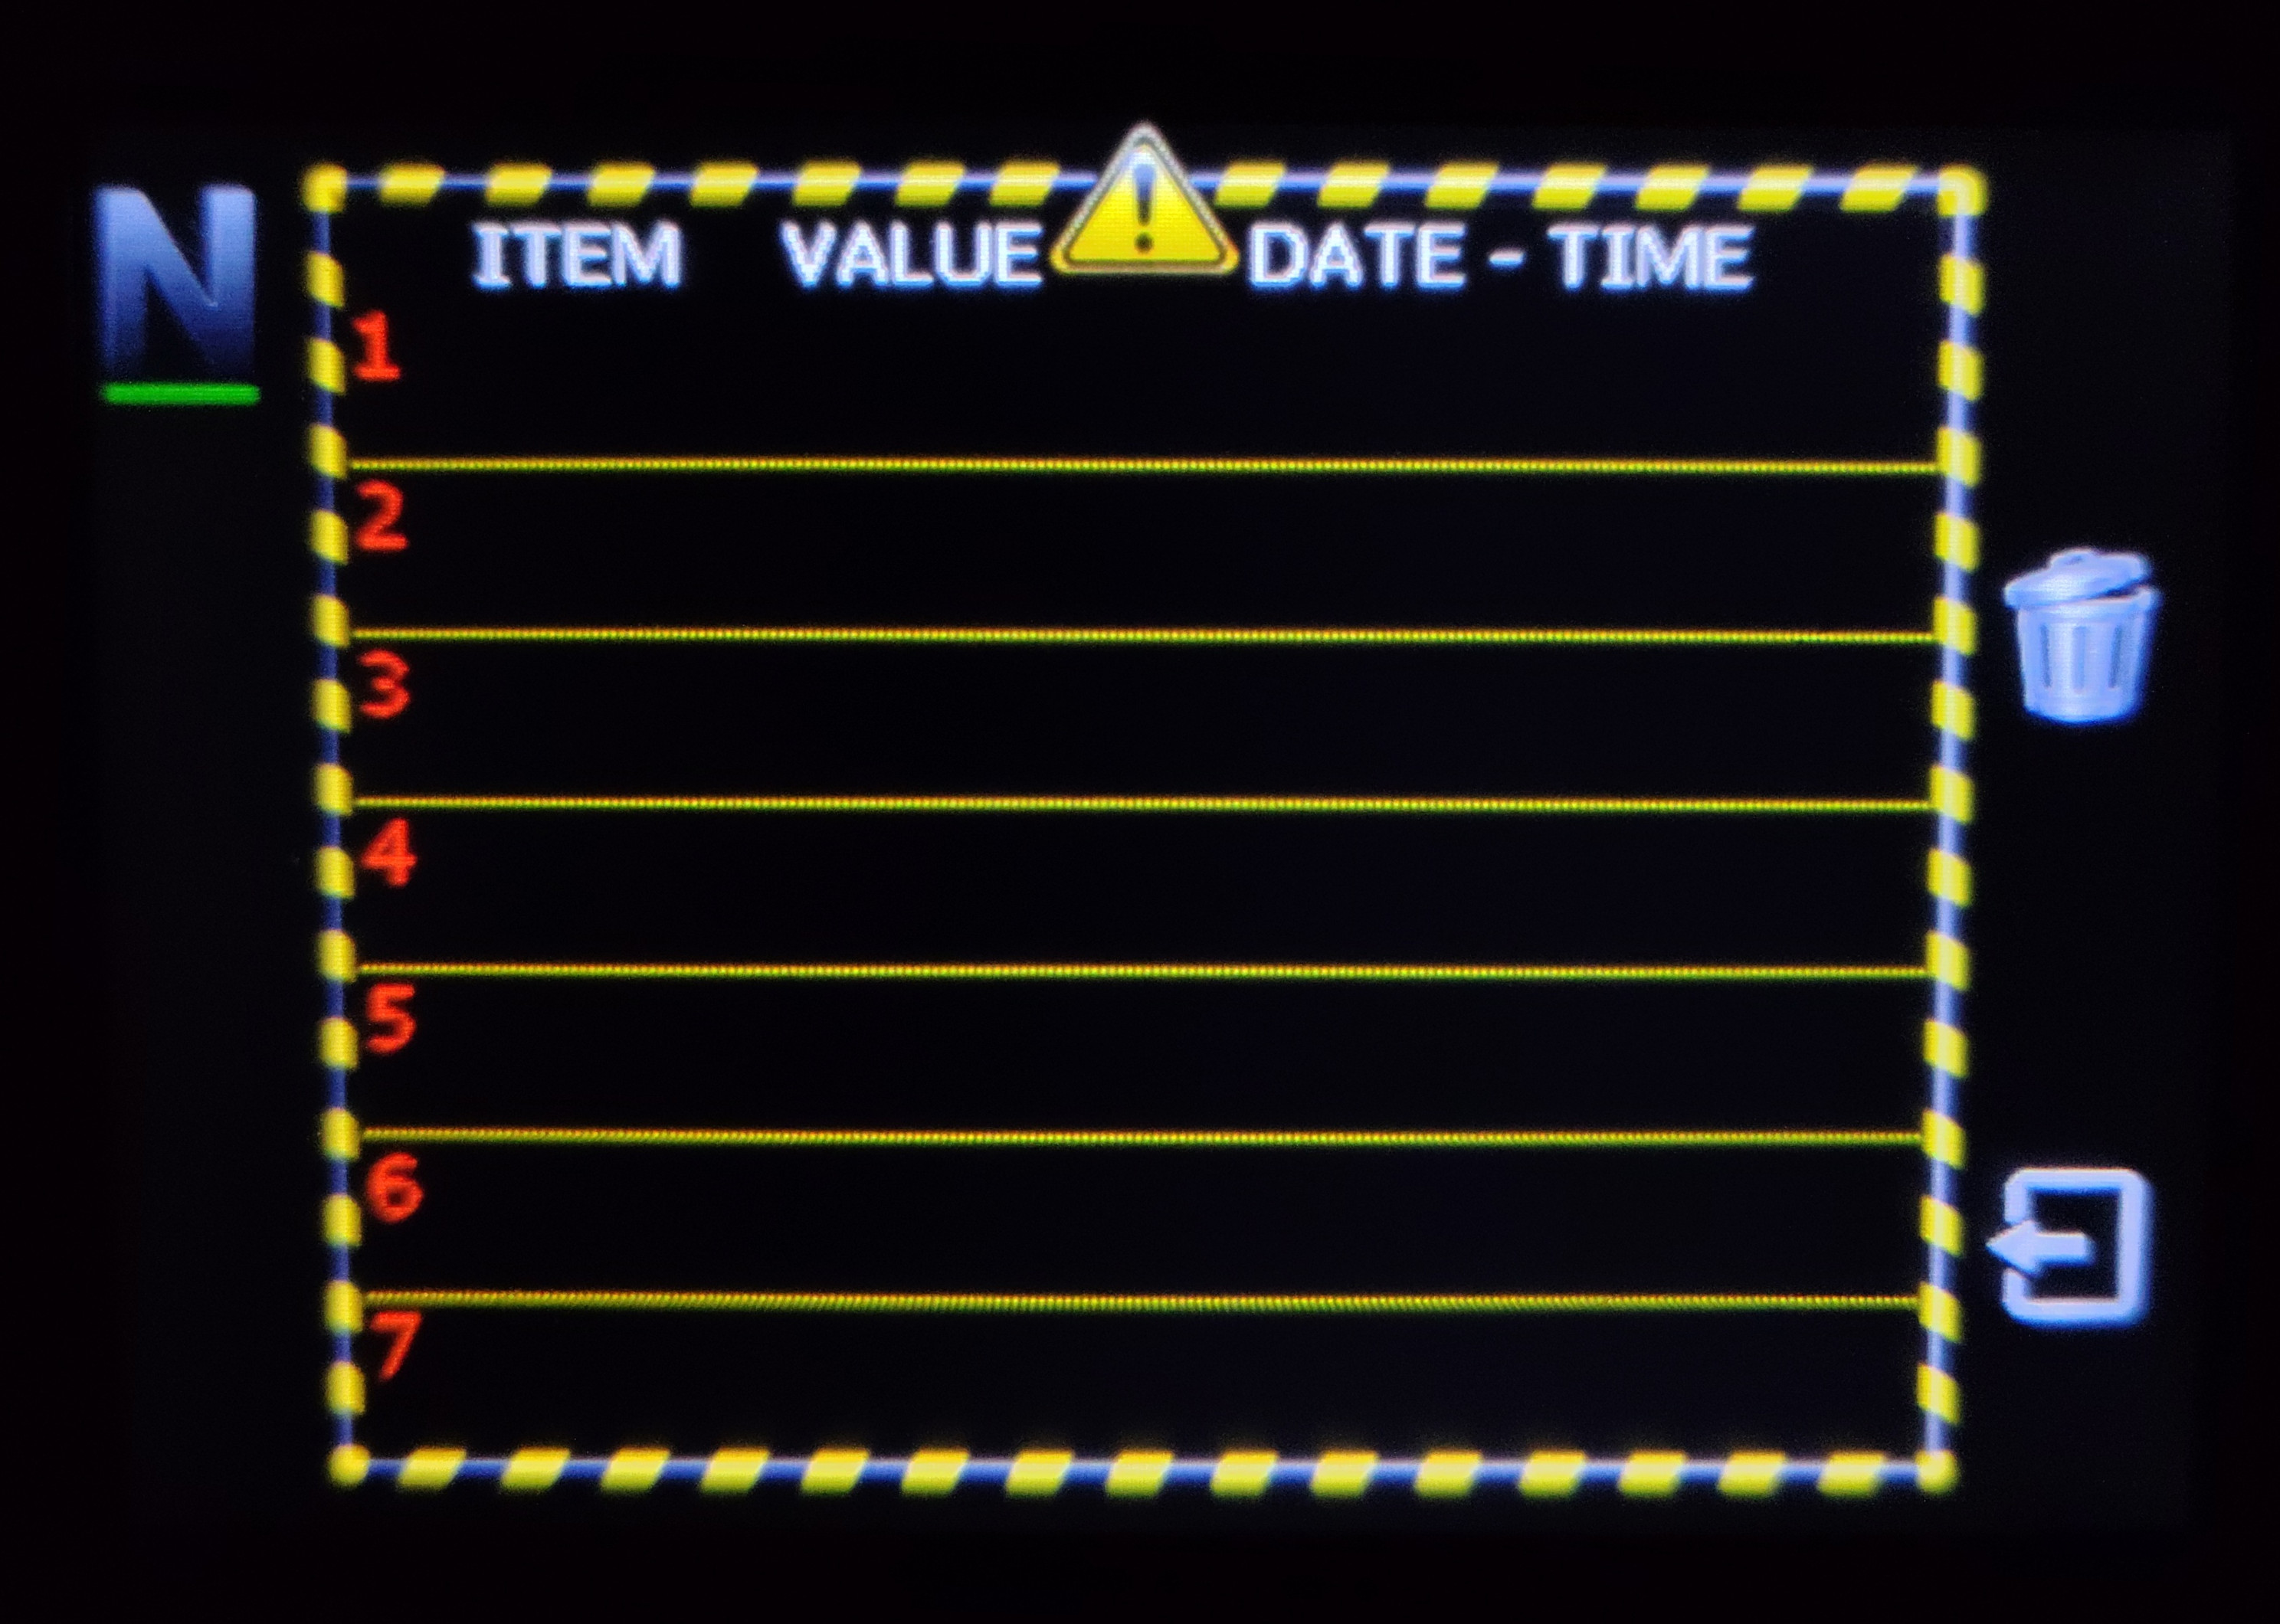
\includegraphics[width=0.8\textwidth]{figures/alarm_page.jpg}
    \caption{La page du journal des alarmes en 3D.}
\end{figure}

L'image montre un petit tableau qui contient l'élément ayant provoqué le déclenchement de l'alarme, associé à son icône et à sa valeur. J'ai ensuite ajouté la date et l'heure (disponibles si connecté à un réseau la première fois) pour savoir quand cet enregistrement a été ajouté à la liste.\\

Dans les images suivantes (avec l'ancien design), la plupart des enregistrements sont liés au SOC de la batterie, spécifiquement lorsqu'il descend en dessous de 30\%. Vous découvrirez comment définir vos propres alarmes sur le serveur web dans la Section~\ref{sec:web_alarm_triggers}.

\begin{figure}[H]
    \centering
    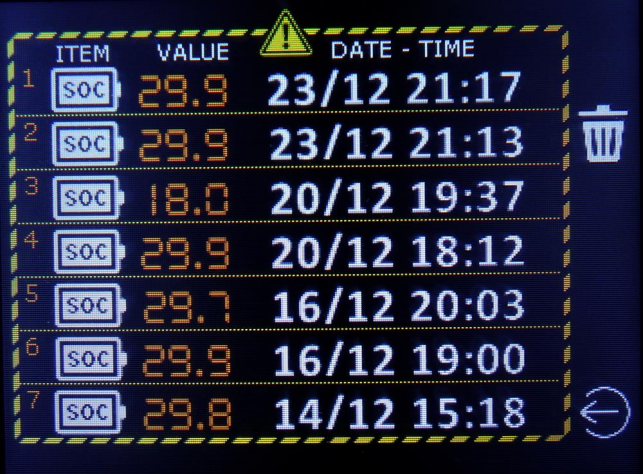
\includegraphics[width=0.7\textwidth]{figures/alarm_log_old1.png}
    \caption{La page du journal des alarmes en 3D.}
\end{figure}

\subsection{Vérification des déclenchements d'alarmes plus anciens}

Si vous avez besoin de voir des déclenchements d'alarmes plus anciens qui n'apparaissent pas dans la liste des sept premiers, vous pouvez appuyer sur l'icône d'avertissement jaune en haut du tableau, ce qui remplacera les valeurs affichées par les plus anciennes. Vous pouvez effectuer cette action deux fois, car ToM est capable de stocker jusqu'à 21 déclenchements d'alarmes et oublie les plus anciens.

\begin{figure}[H]
    \centering
    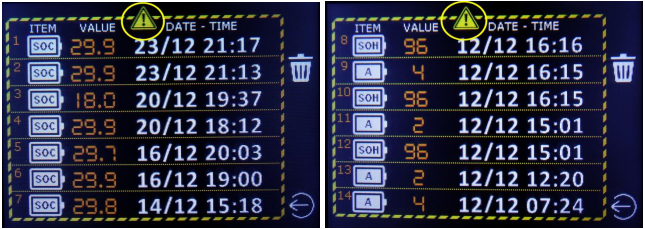
\includegraphics[width=1\textwidth]{figures/alarm_log_old2.png}
    \caption{Changement des déclenchements affichés.}
\end{figure}

Comme vous pouvez le voir sur ces deux photos de la page du journal des alarmes, lorsque j'ai appuyé sur le bouton d'avertissement jaune entouré, les données affichées ont changé pour laisser place à des données plus anciennes, comme vous pouvez le constater en comparant les dates. Le compteur d'éléments sur la gauche a également changé (8--14).

\subsection{Suppression d'un déclencheur d'alarme}
\label{sec:delete_log_record}

Si vous n'avez plus besoin d'un ou plusieurs enregistrements, vous pouvez choisir d'en supprimer certains. Sélectionnez un ou plusieurs enregistrements à supprimer définitivement en appuyant sur leur date ou leur heure (une petite coche rouge apparaîtra à côté des enregistrements choisis). Appuyez ensuite sur l'icône de corbeille entourée de jaune sur la deuxième photo pour supprimer les enregistrements sélectionnés. Ces enregistrements disparaîtront et seront remplacés par les enregistrements suivants, provoquant un décalage de l'ensemble de la liste comme vous pouvez le remarquer sur la deuxième image.

\begin{figure}[H]
    \centering
    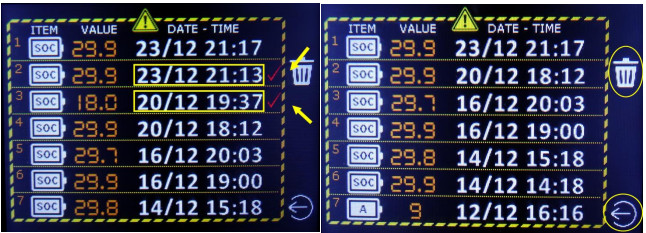
\includegraphics[width=1\textwidth]{figures/alarm_log_old3.jpg}
    \caption{Suppression des déclenchements d'alarmes sélectionnés.}
\end{figure}

Sur cette page, il n'y a pas de barre d'icônes d'état ni de boutons pour changer de page, puisqu'il s'agit d'une page de configuration qui n'a pas besoin de telles commandes. Pour quitter, appuyez sur le bouton fléché dans le coin inférieur droit et ToM vous ramènera à la page où vous étiez avant de consulter la page du journal des alarmes, à partir de laquelle vous pourrez à nouveau modifier la page active.

\section{La page du trajet}
\label{sec:trip_page}

Cette page est capable de stocker les données d'un trajet \textit{(un trajet correspond au temps écoulé entre le moment où vous commencez à conduire et celui où vous éteignez votre Twizy)} puis de décider de conserver ou de rejeter ces valeurs lorsque vous recommencez à conduire. Vous pouvez enregistrer simultanément jusqu'à cinq données de trajet. La disposition est la même que celle de la page principale, les commandes permettant de modifier l'ordre des valeurs ou les données au premier plan ont donc déjà été abordées dans la Section~\ref{sec:main-layout}. Les paragraphes suivants expliquent comment réinitialiser un trajet et comment changer le trajet en cours.

\begin{figure}[H]
    \centering
    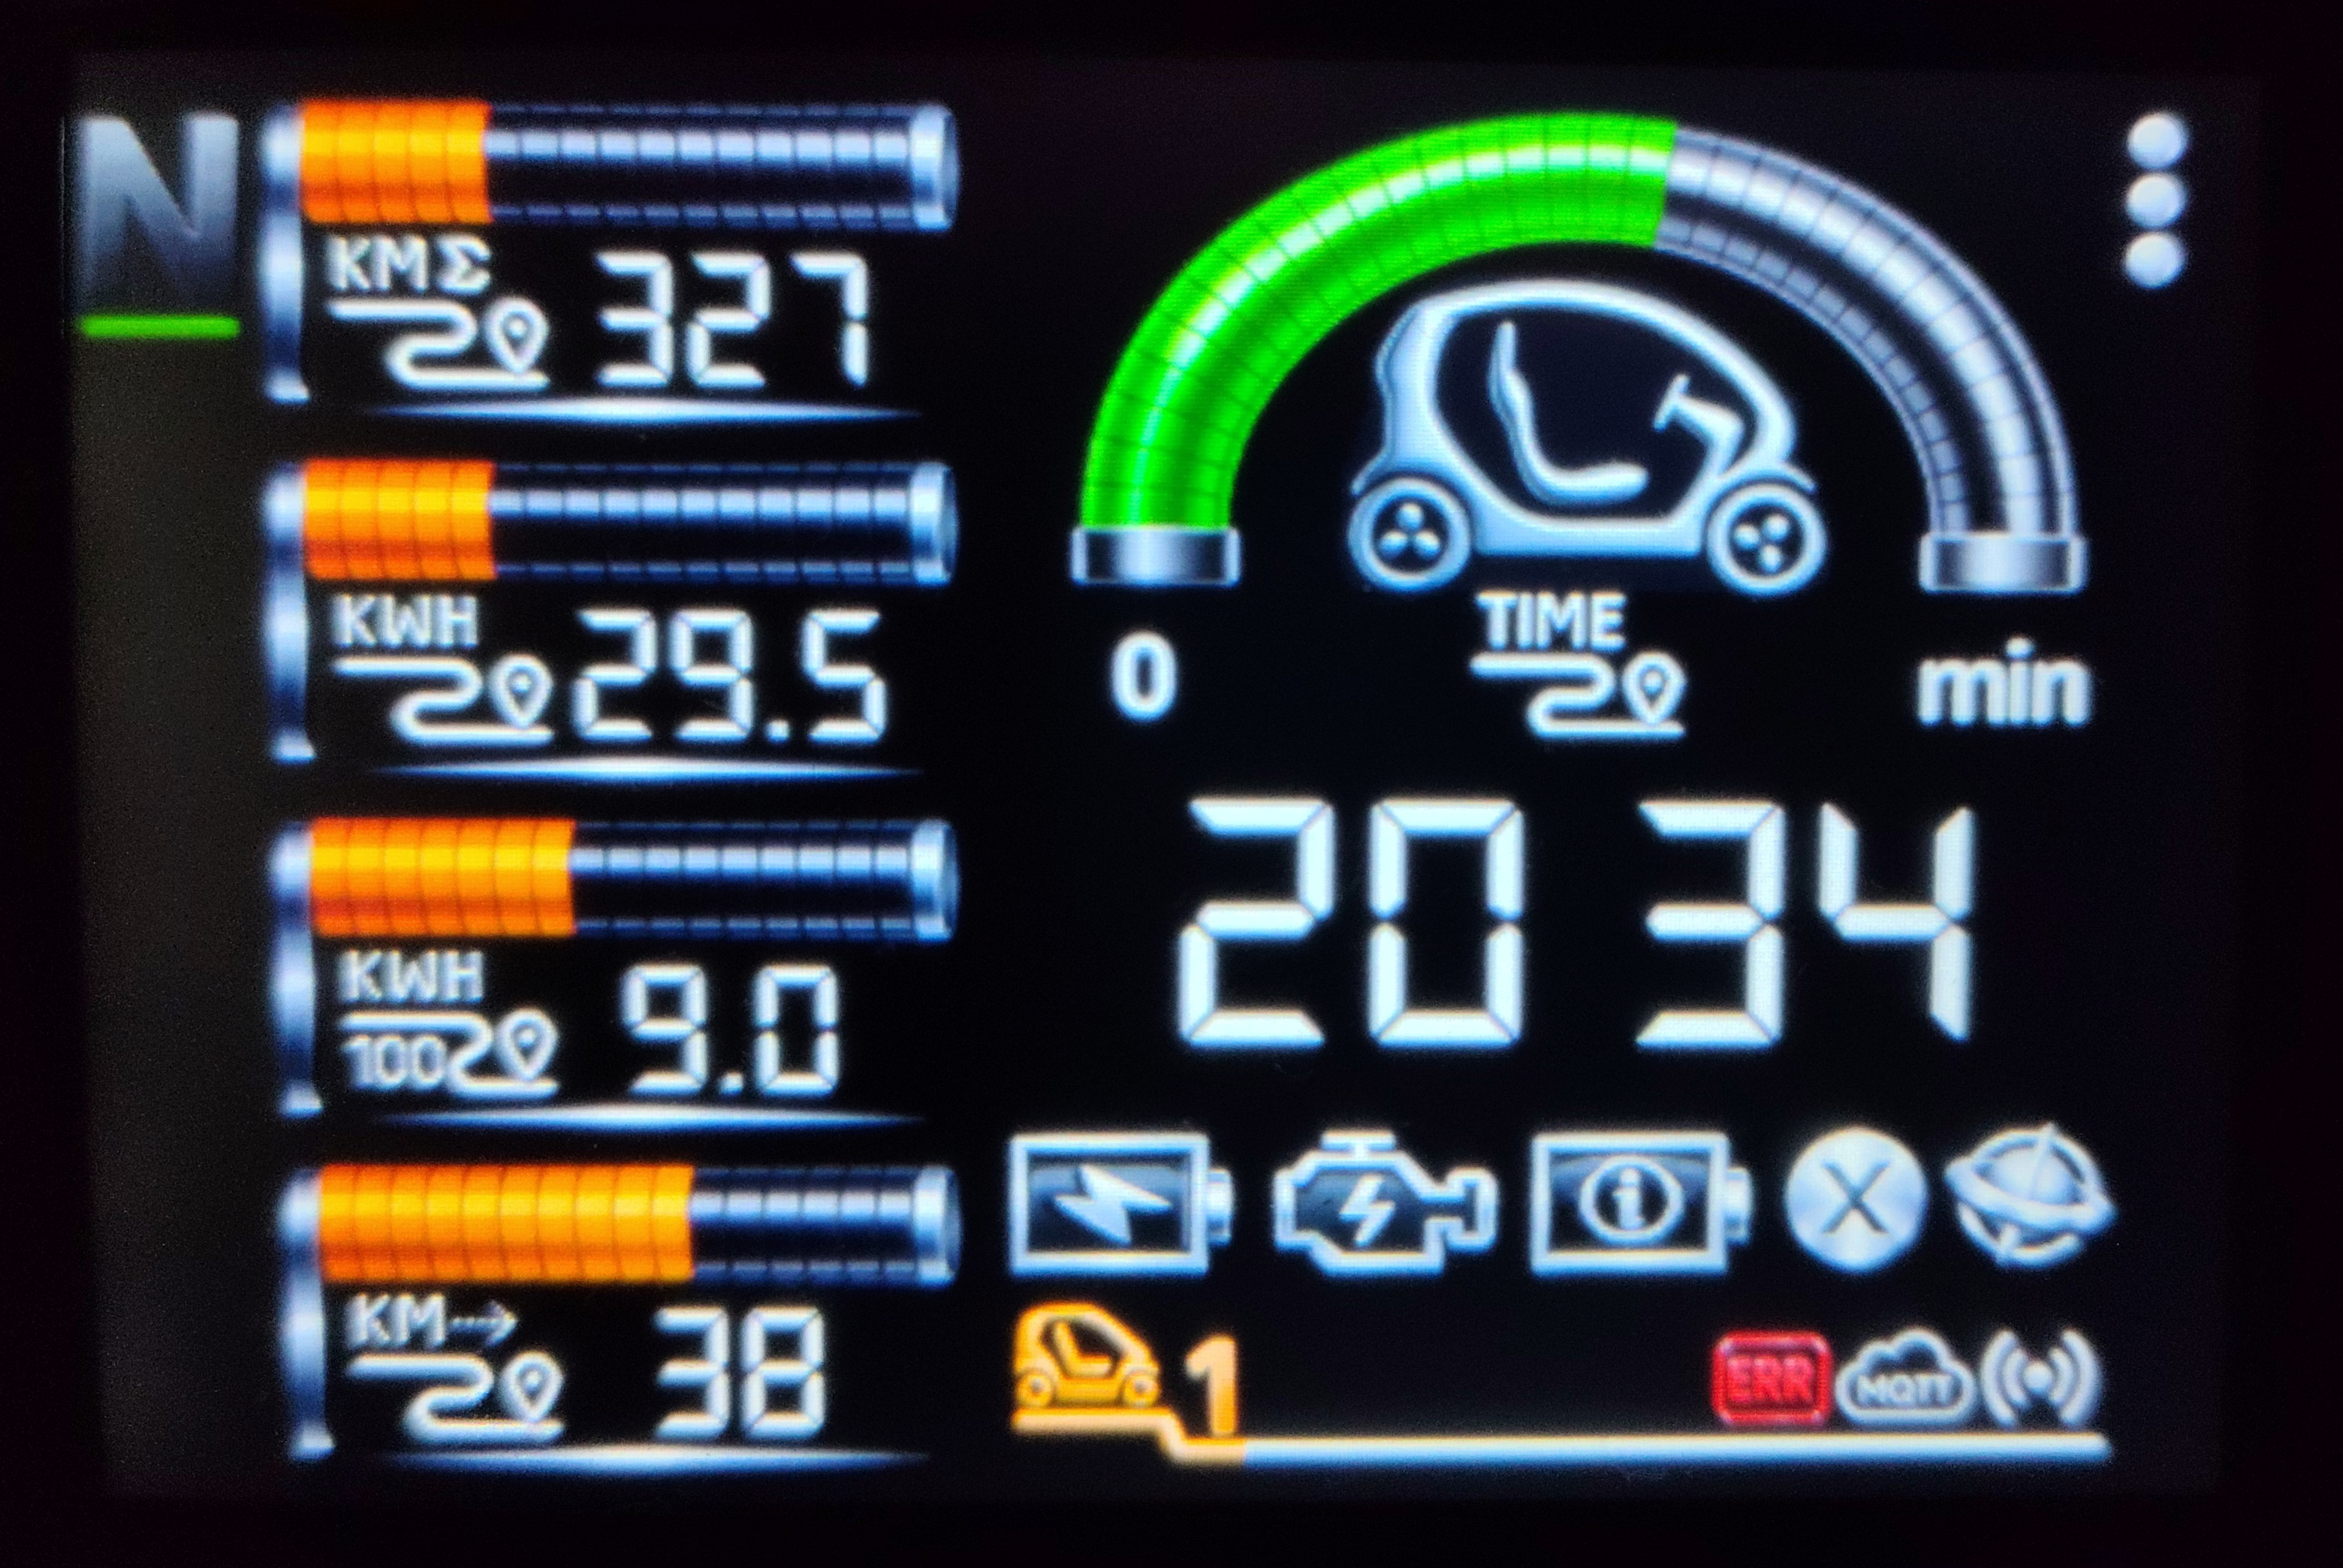
\includegraphics[width=0.8\textwidth]{figures/trip_page_full.jpg}
    \caption{La page du trajet.}
\end{figure}

\subsection{Changer le trajet en cours}

Si vous souhaitez commencer à enregistrer les données sur un trajet spécifique choisi de 1 à 5, vous pouvez appuyer sur l'icône de trajet entourée de jaune dans l'image précédente. Lorsque vous appuyez dessus pour la première fois, vous serez dirigé vers le trajet n° 1 et des appuis successifs feront défiler tous les trajets disponibles, afin que vous puissiez sélectionner celui que vous souhaitez démarrer ou poursuivre.\\

Pour voir sur quel trajet ToM enregistre actuellement, reportez-vous au chiffre orange sur l'icône de trajet. Une fois le trajet désiré choisi, vous pouvez également changer la page active si vous le souhaitez, sans perdre le trajet sélectionné, car ToM continuera d'enregistrer les valeurs même si la page du trajet n'est pas affichée à l'écran.

\subsection{Désactiver l'enregistrement du trajet}

Dans cet exemple, je suis actuellement sur la page moteur et j'enregistre les données sur la cinquième page de trajet, comme l'indique le petit chiffre orange près de l'icône du trajet. Si vous souhaitez mettre en pause l'enregistrement du trajet, vous pouvez le faire sur ToM+ en \textbf{maintenant enfoncé pendant trois secondes le bouton de trajet} pendant qu'une autre page est active (dans cet exemple, celle de la batterie).\\

\begin{figure}[ht]
    \centering

    \begin{subfigure}[t]{0.48\textwidth}
        \centering
        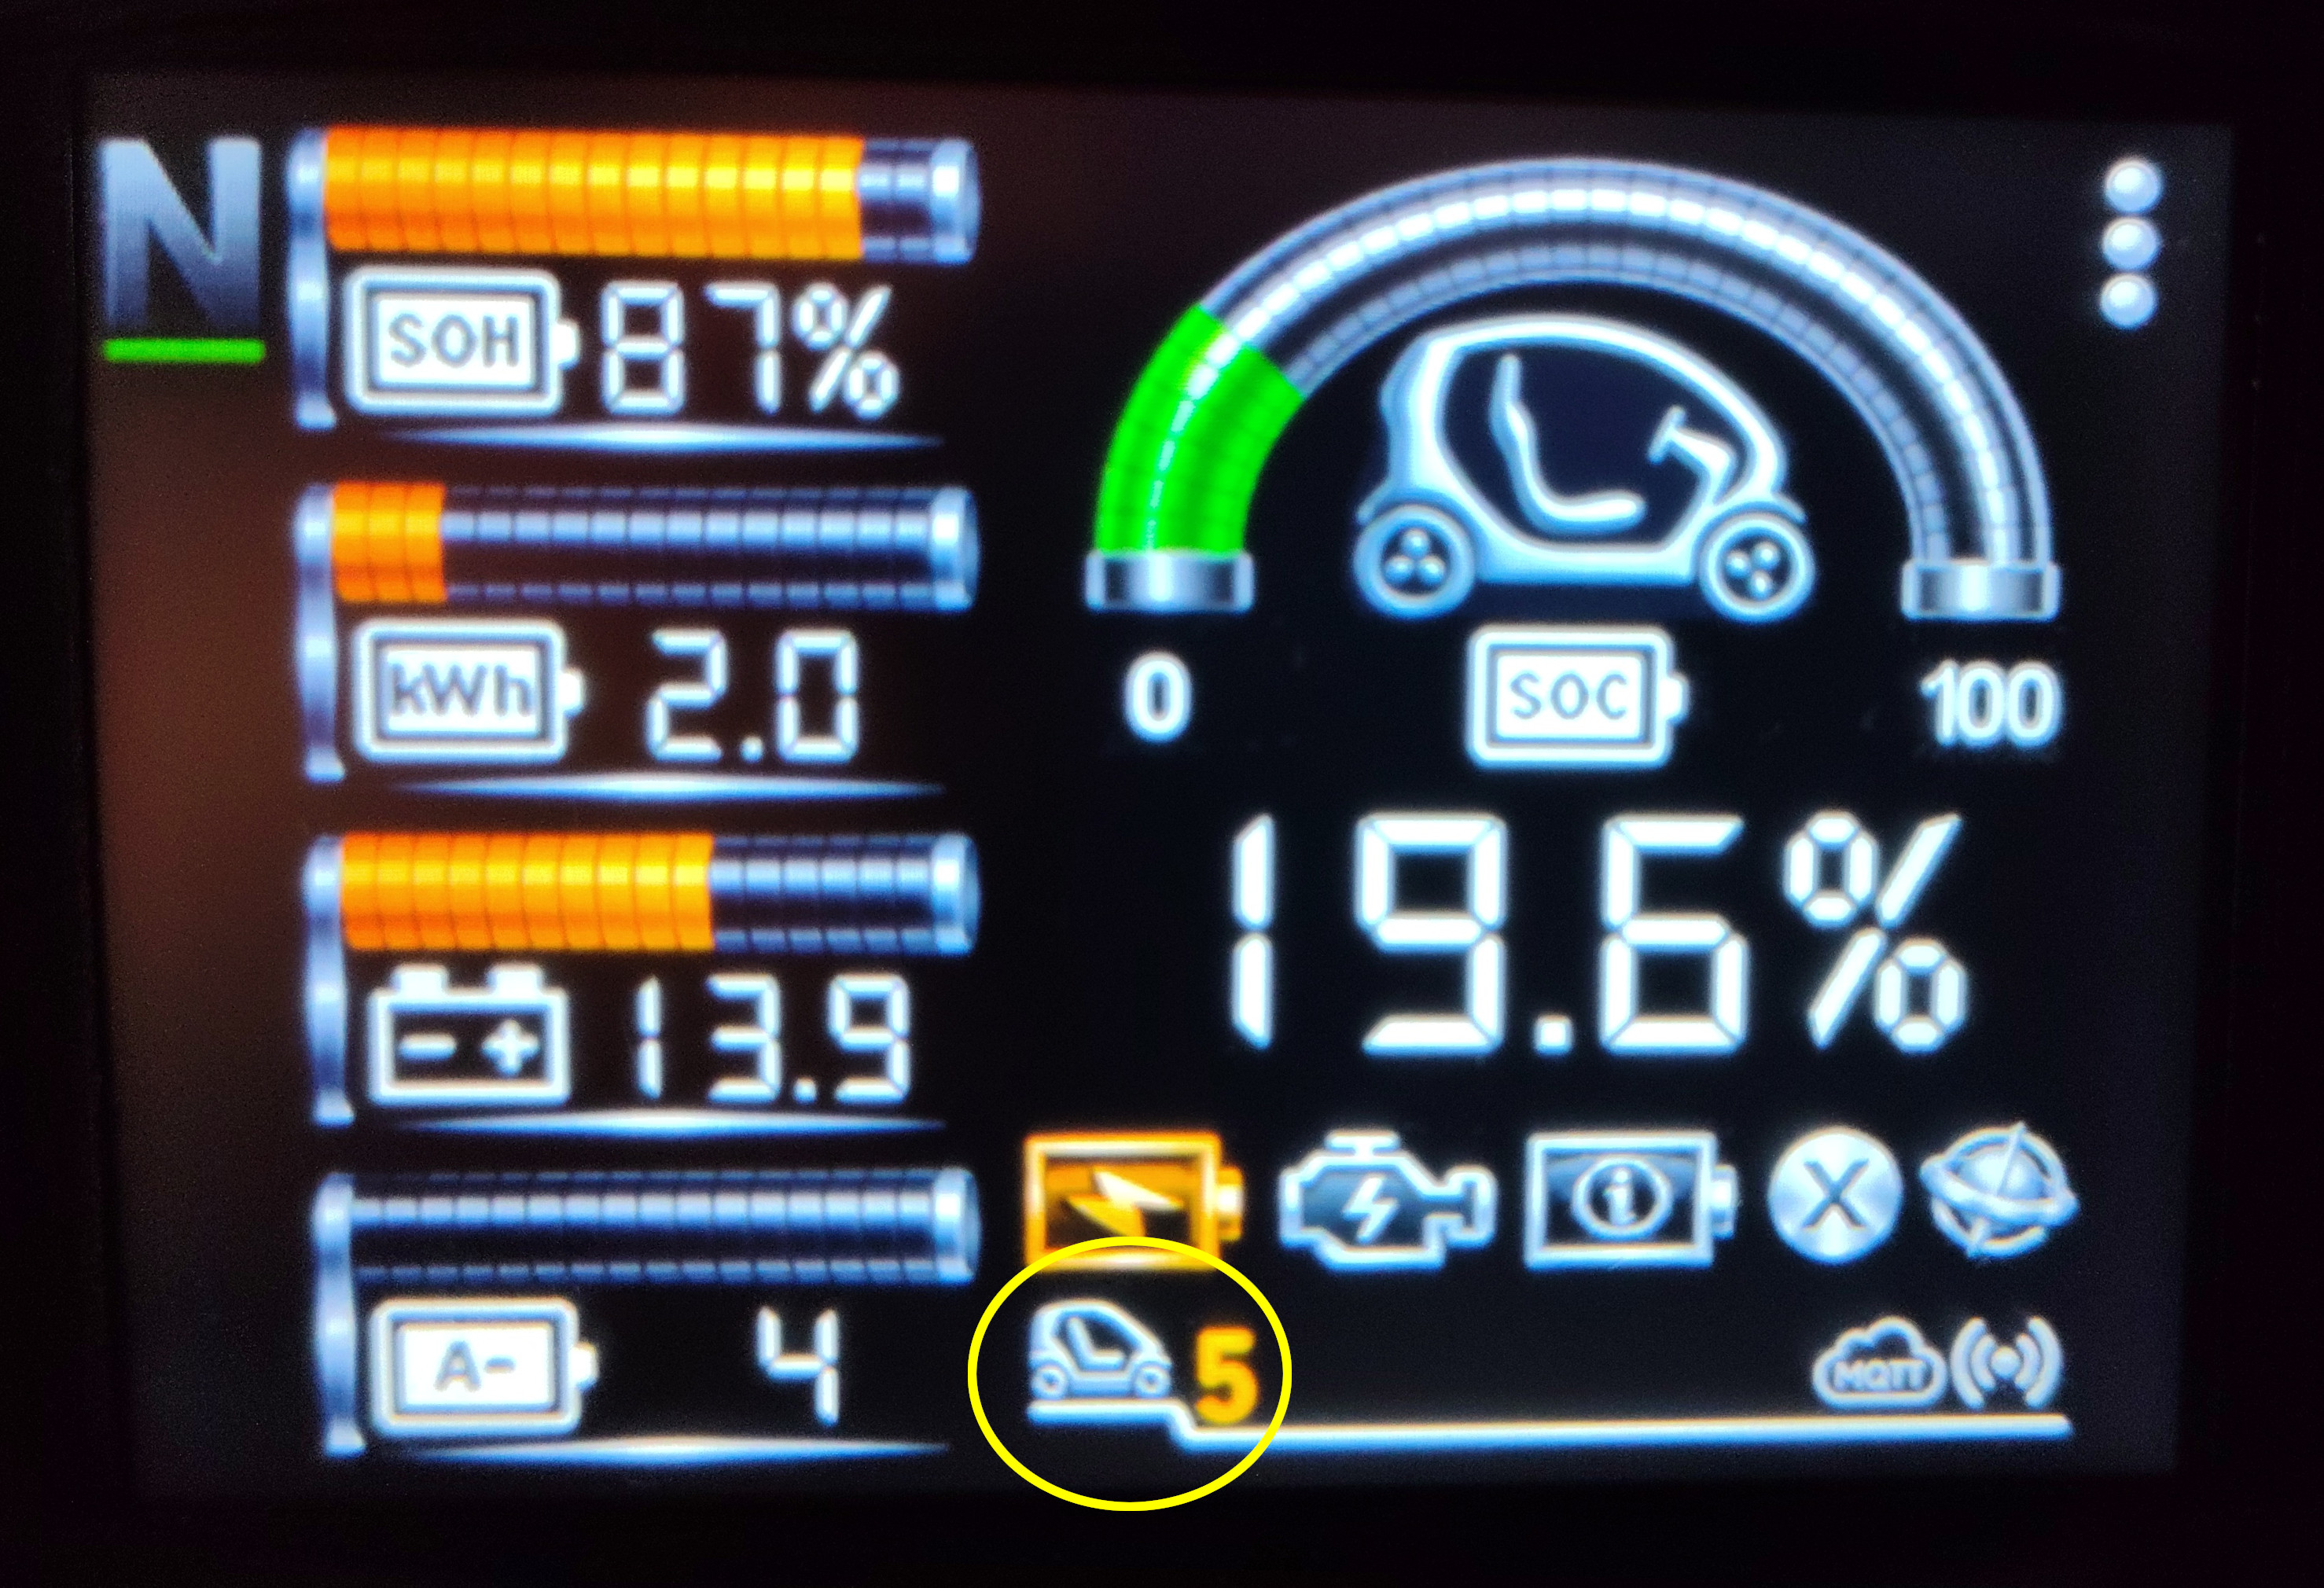
\includegraphics[width=\linewidth]{figures/trip_page_on.jpg}
        \caption{Enregistrement de trajet actif sur le trajet 5.}
    \end{subfigure}
    \hfill
    \begin{subfigure}[t]{0.48\textwidth}
        \centering
        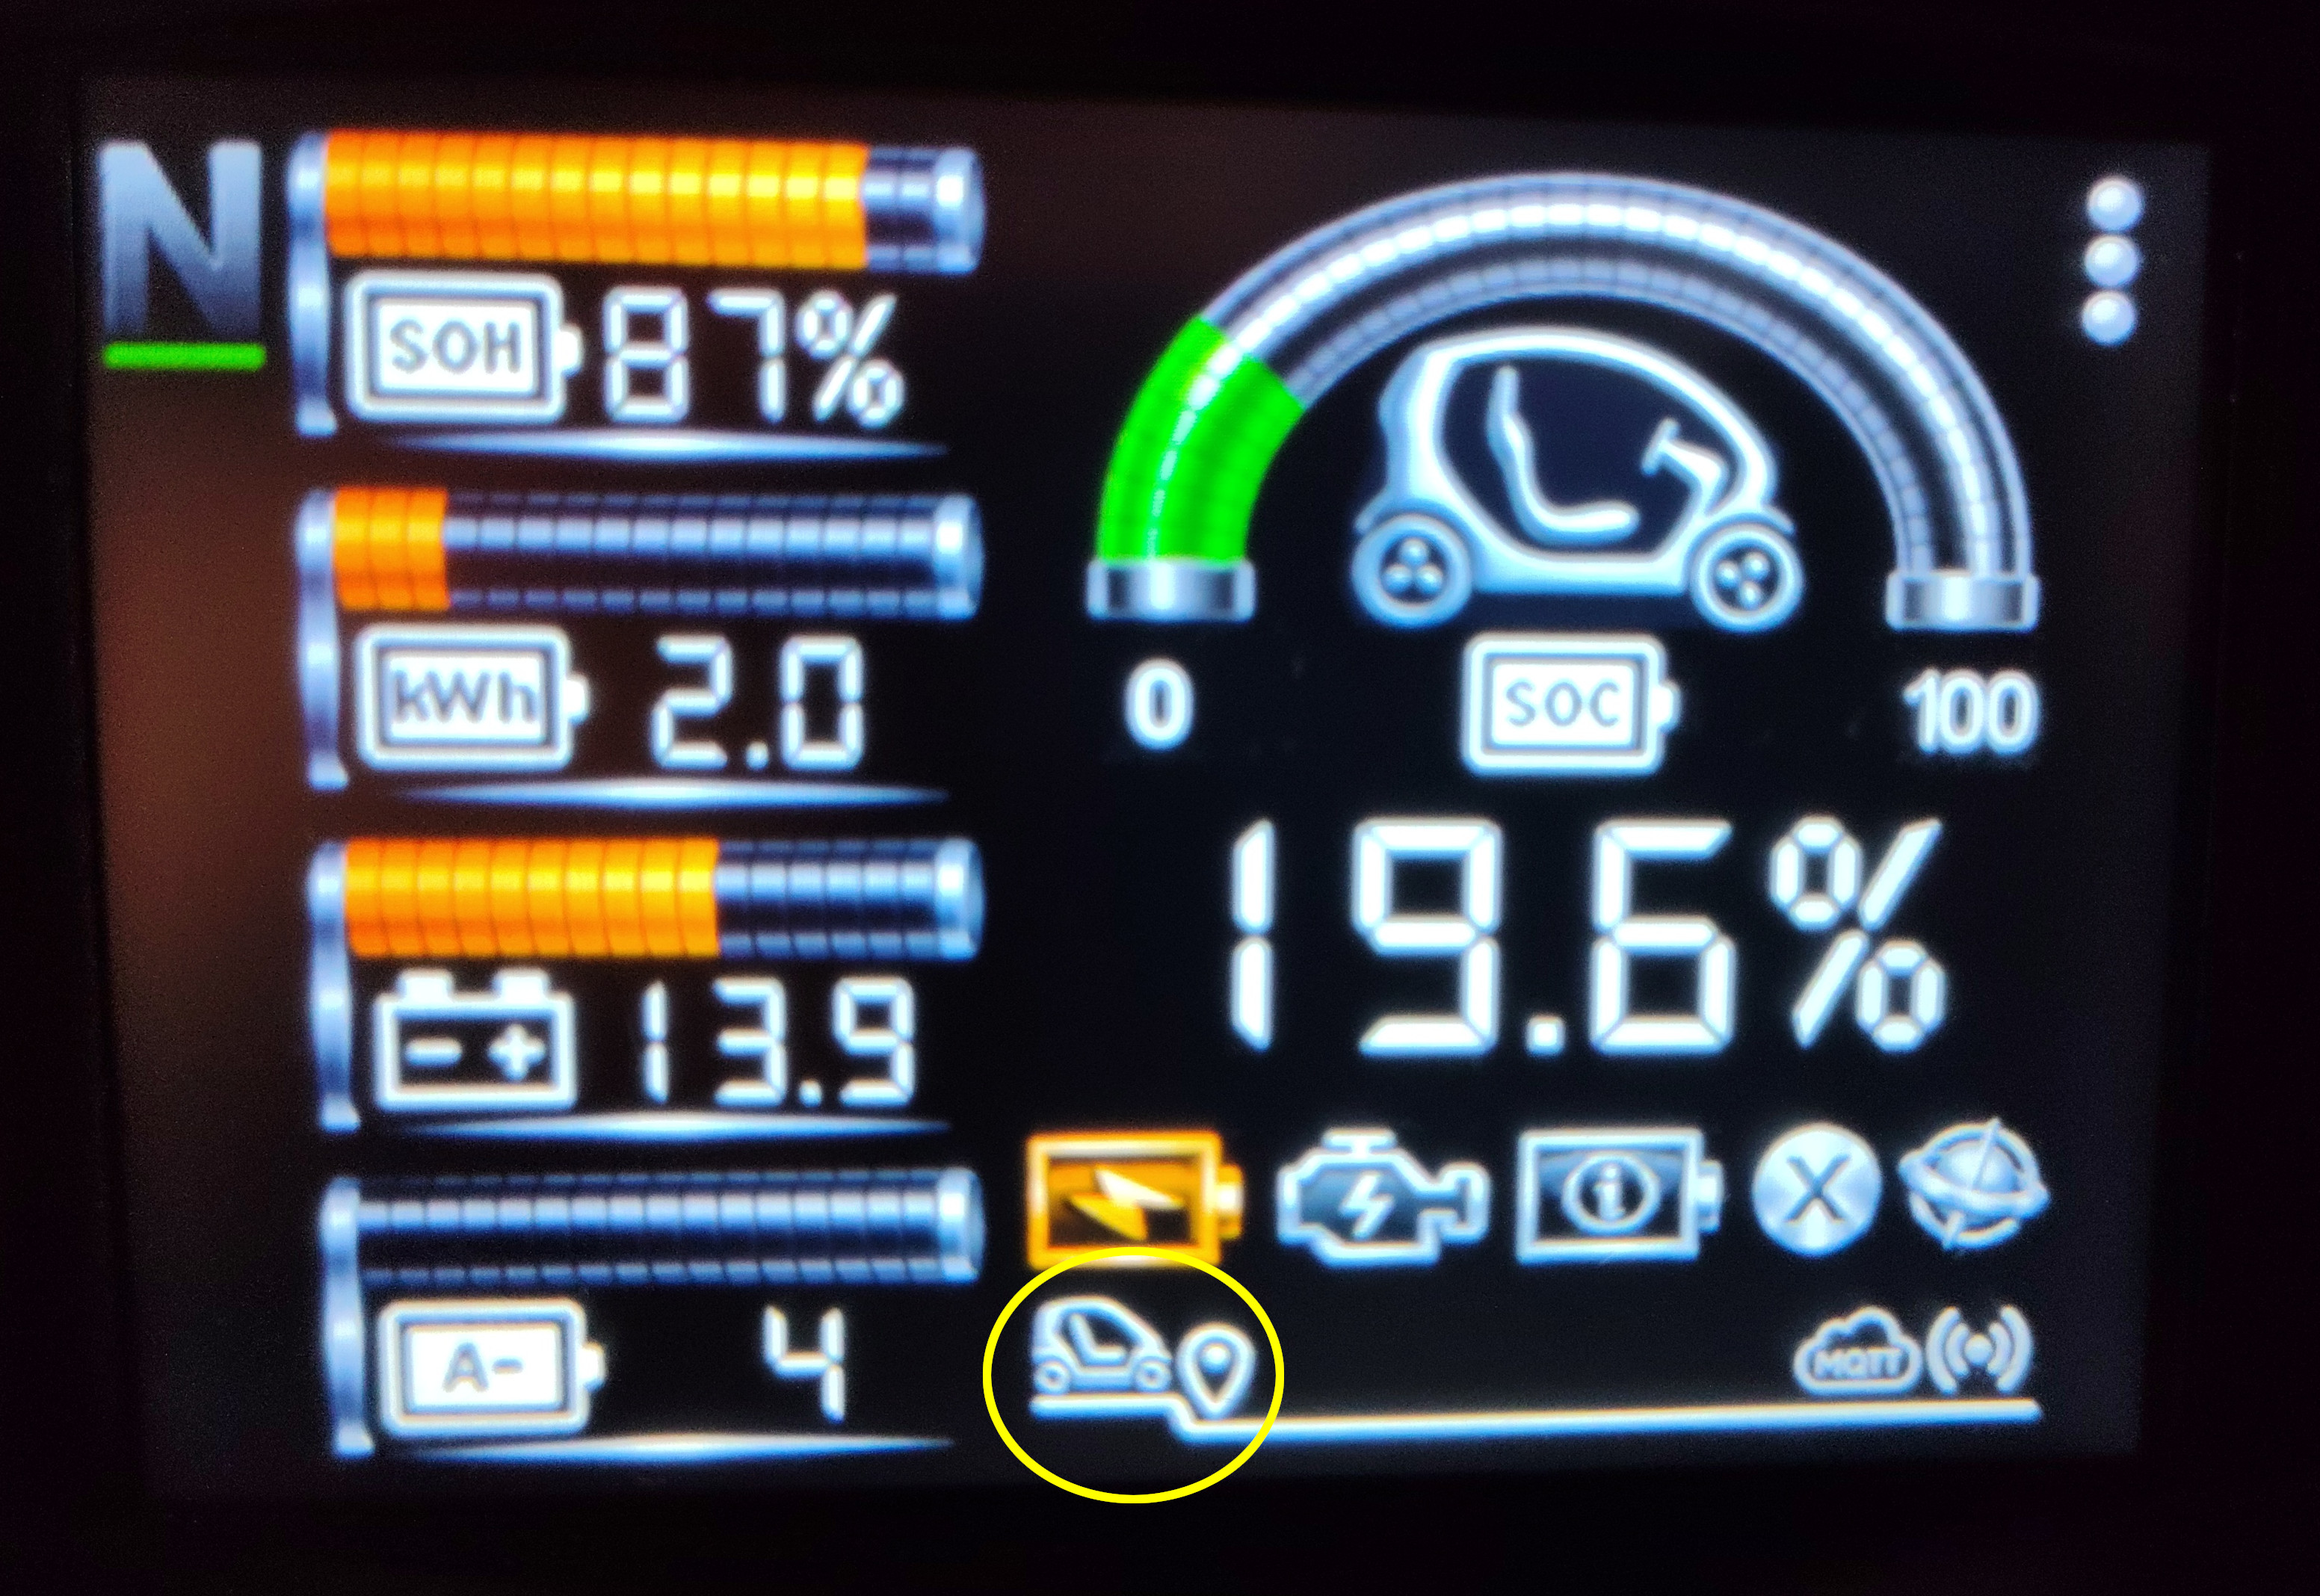
\includegraphics[width=\linewidth]{figures/trip_page_off.jpg}
        \caption{Enregistrement de trajet en pause.}
    \end{subfigure}
\end{figure}

Une fois relâché, ToM+ modifie la petite icône de trajet pour afficher le symbole de carte au lieu du numéro de trajet, afin de vous informer qu'il n'enregistre plus les données (deuxième image). Lorsque vous êtes prêt à reprendre l'enregistrement du trajet, appuyez sur la page du trajet jusqu'à trouver le trajet souhaité en faisant défiler tous ceux disponibles.

\subsection{Réinitialiser un trajet}

Si vous souhaitez effacer les données d'un trajet spécifique, vous pouvez le sélectionner et \textbf{maintenir enfoncé le bouton du trajet pendant trois secondes}. Une fois relâché, vous devriez remarquer que toutes les valeurs du trajet sur la page ont été réinitialisées (généralement à zéro). La différence entre cette action et la précédente est que dans ce cas, les données du trajet sont effacées, tandis que dans la précédente, les données du trajet sont simplement mises en pause. De plus, vous devez ici être sur la page du trajet, alors que pour la précédente, vous devez être sur n'importe quelle autre page.

\clearpage

\section{La page de l'historique des trajets}
\label{sec:trip_history}

Cette page stocke les données des vingt derniers trajets et sa disposition est la même que celle du journal des alarmes. Les valeurs sont mises à jour et enregistrées uniquement lorsque le trajet sélectionné est le \textbf{numéro 5}.

\subsection{Comment accéder à la page de l'historique des trajets}

Cette page n'est pas accessible depuis la page principale, mais vous pouvez y accéder en \textbf{appuyant longuement sur l'icône du journal des alarmes} sur la ligne inférieure de l'écran jusqu'à ce qu'elle change. En effet, la page d'historique des trajets n'est pas une page que vous utiliserez souvent, il a donc été décidé de la masquer de la page principale pour gagner de l'espace, tout comme la page d'erreur. Ainsi, la séquence de pages disponibles en \textbf{appuyant longuement sur l'icône du journal des alarmes} est : page du journal des alarmes (Section~\ref{sec:alarm_log}) $\rightarrow$ page d'erreur (Section~\ref{sec:error_page}) $\rightarrow$ page de l'historique des trajets $\rightarrow$ retour à la page du journal des alarmes, chacune avec son icône respective.\\

\begin{figure}[H]
    \centering
    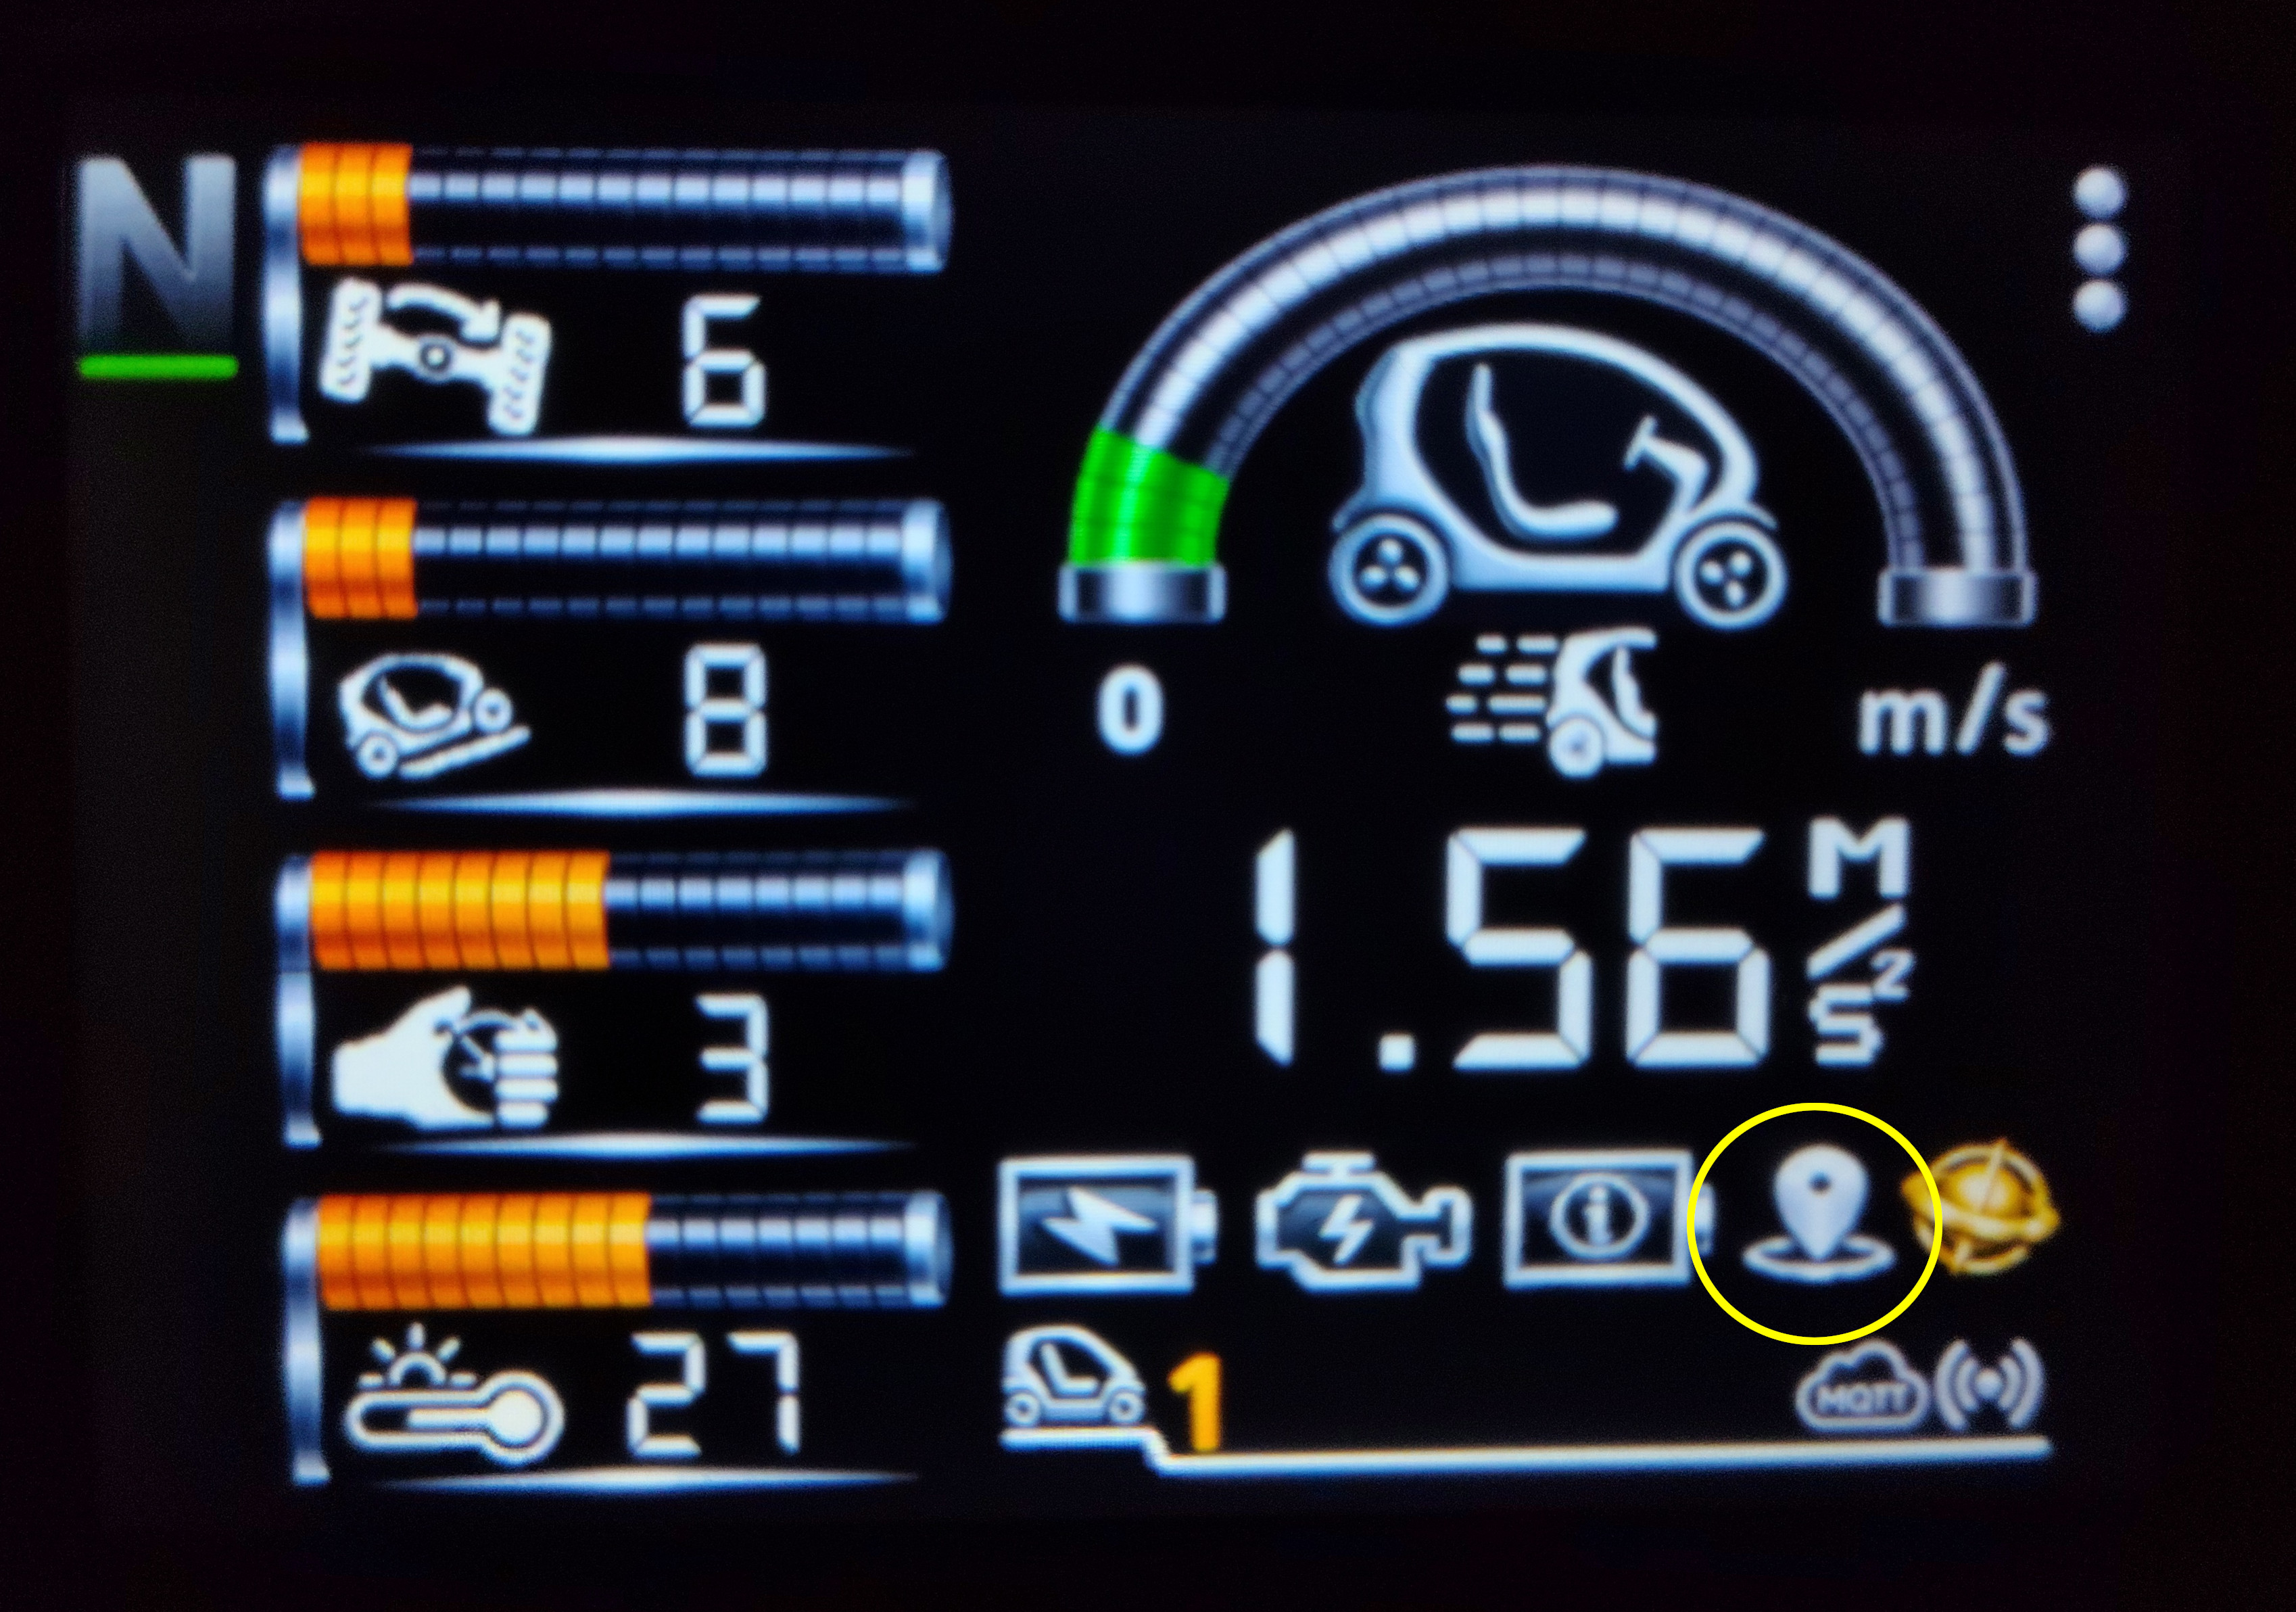
\includegraphics[width=0.8\textwidth]{figures/enter_trip_log_page.jpg}
    \caption{L'icône pour accéder à la page de l'historique des trajets.}
\end{figure}

\subsection{Commandes principales de la page d'historique des trajets}

\begin{figure}[H]
    \centering
    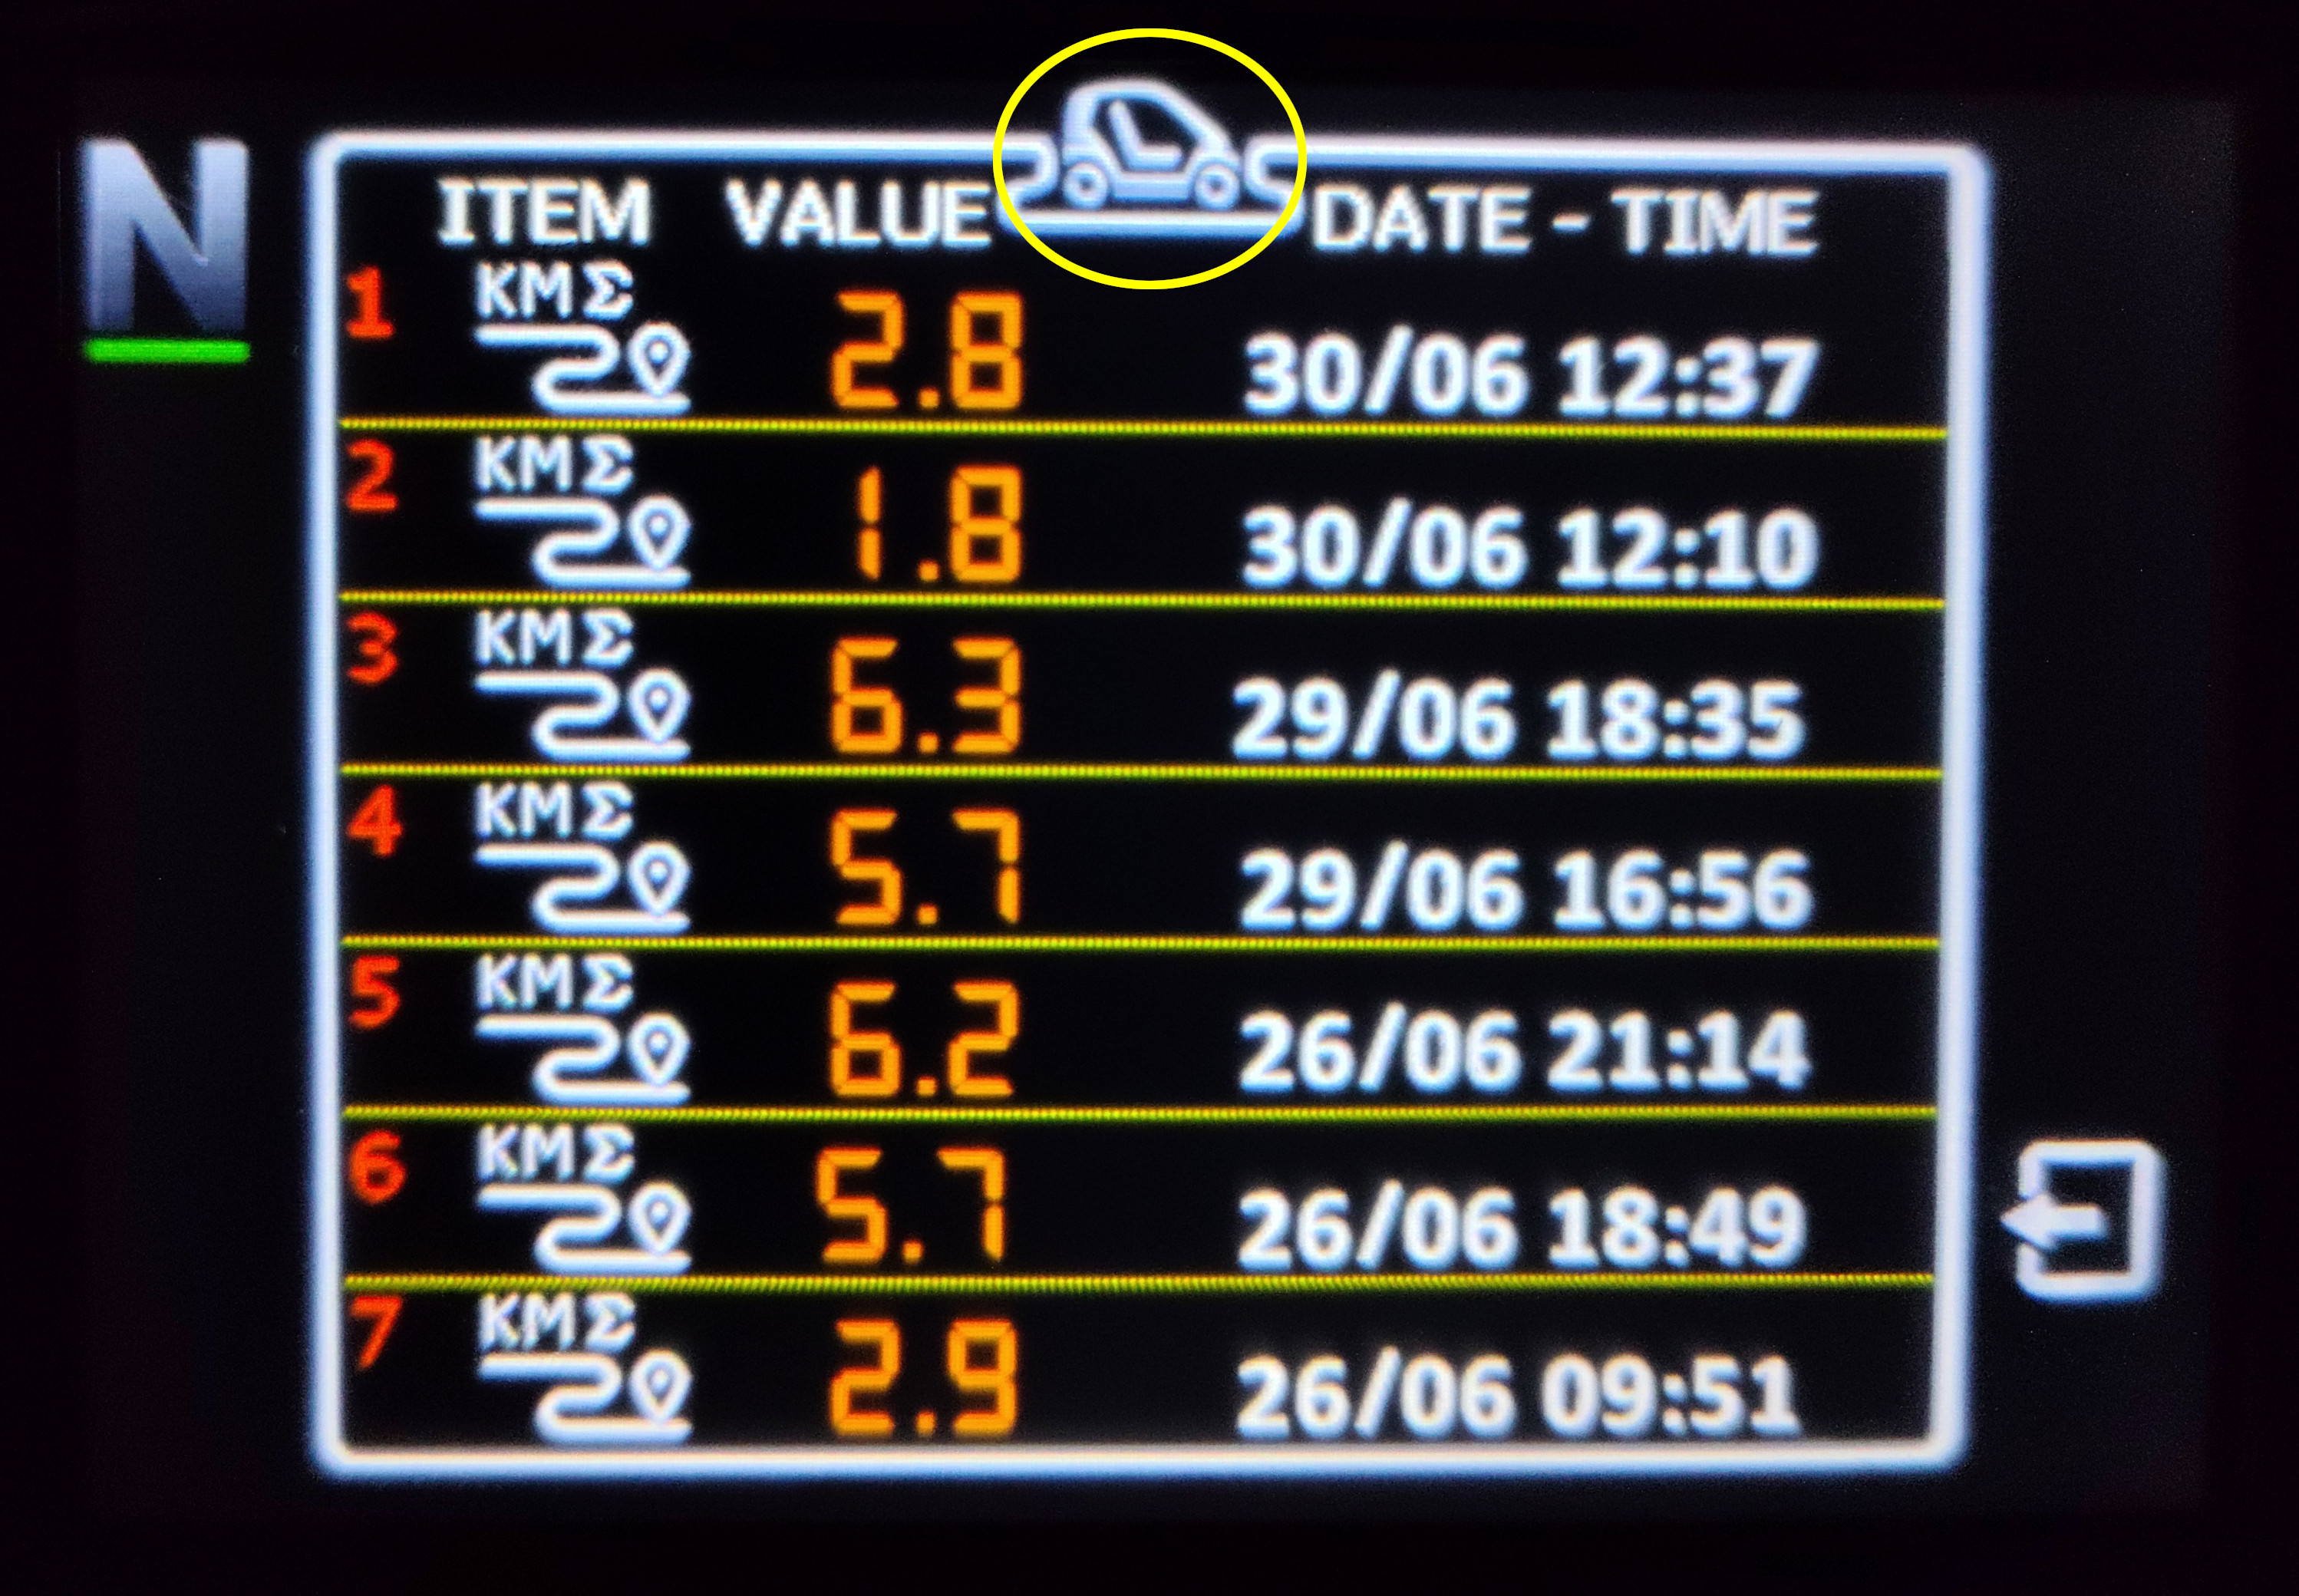
\includegraphics[width=0.8\textwidth]{figures/trip_history_page.jpg}
    \caption{La page de l'historique des trajets.}
\end{figure}

Sur cette image, vous pouvez voir les sept premiers trajets enregistrés dans la liste, avec leur date et heure, ainsi que la distance parcourue. Vous pouvez facilement modifier la donnée affichée sur chaque ligne en appuyant sur l'icône de la donnée comme indiqué ci-dessous. Les données défileront parmi la plupart des données de trajet disponibles, vous permettant de choisir celle à afficher. Dans les images suivantes, vous pouvez voir la même page avec la consommation d'énergie du trajet et la vitesse moyenne.

\begin{figure}[ht]
    \centering

    \begin{subfigure}[t]{0.48\textwidth}
        \centering
        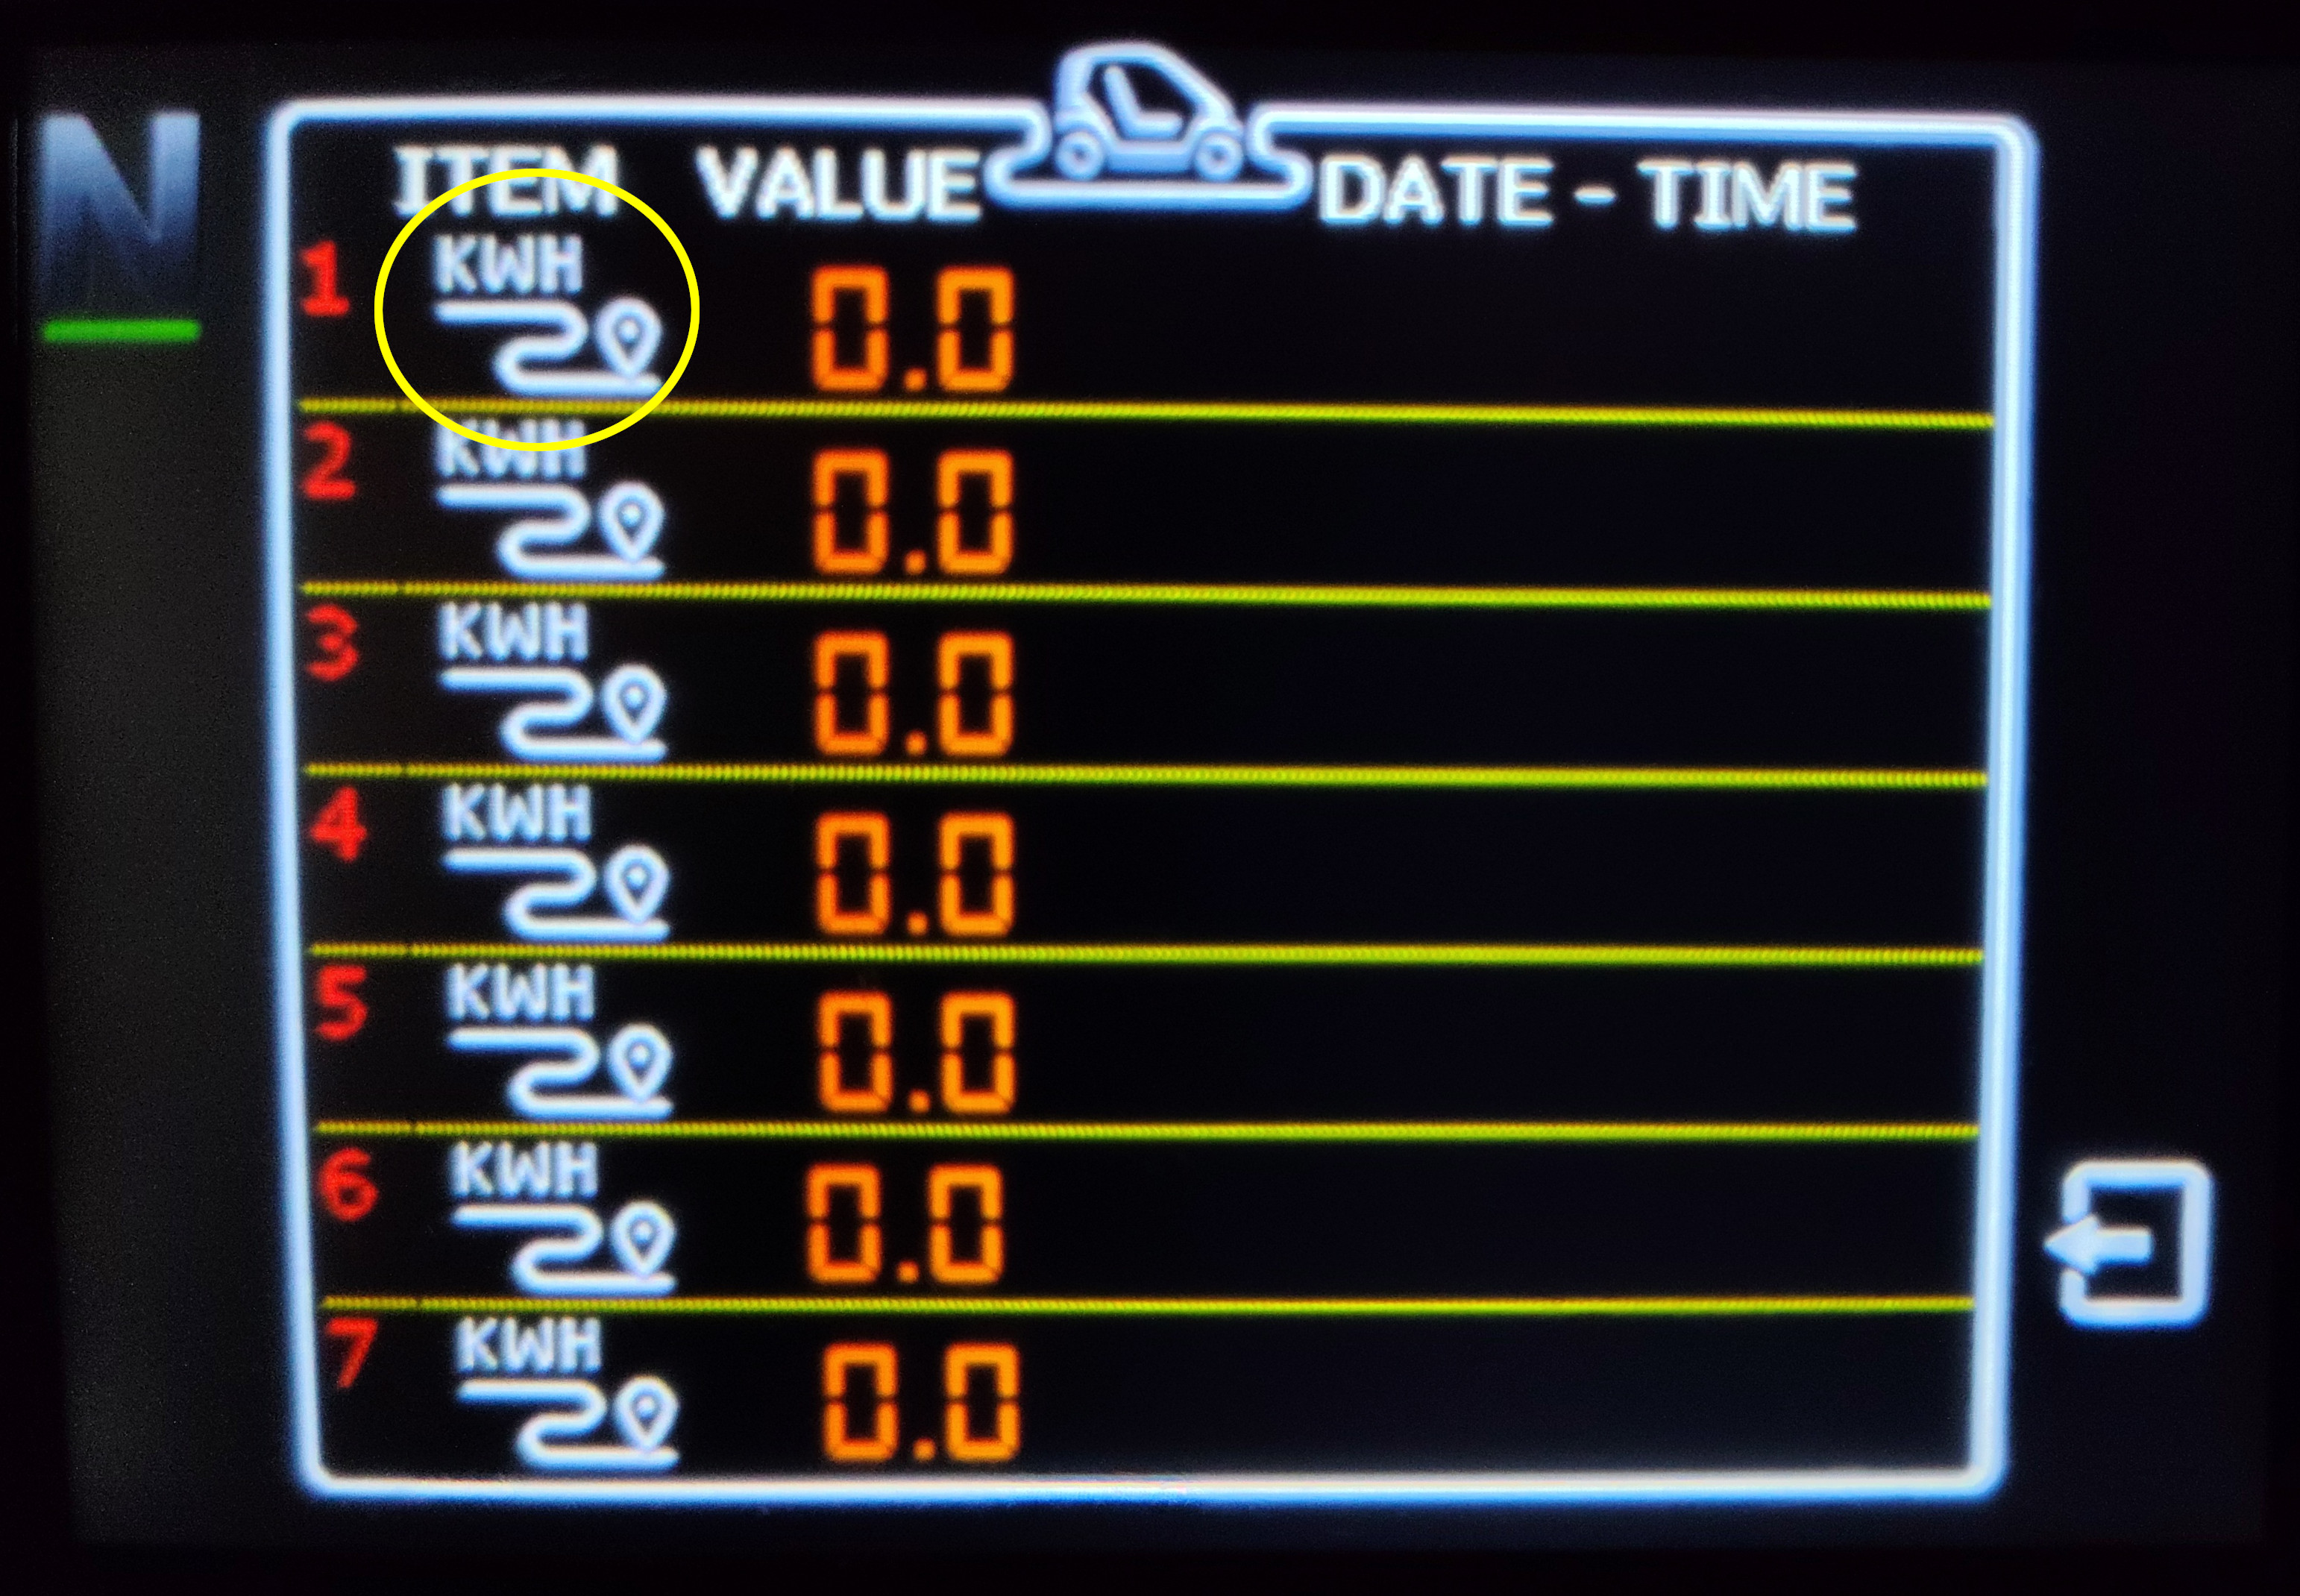
\includegraphics[width=\linewidth]{figures/trip_log_kwh.jpg}
        \caption{Affichage de la consommation d'énergie du trajet.}
    \end{subfigure}
    \hfill
    \begin{subfigure}[t]{0.48\textwidth}
        \centering
        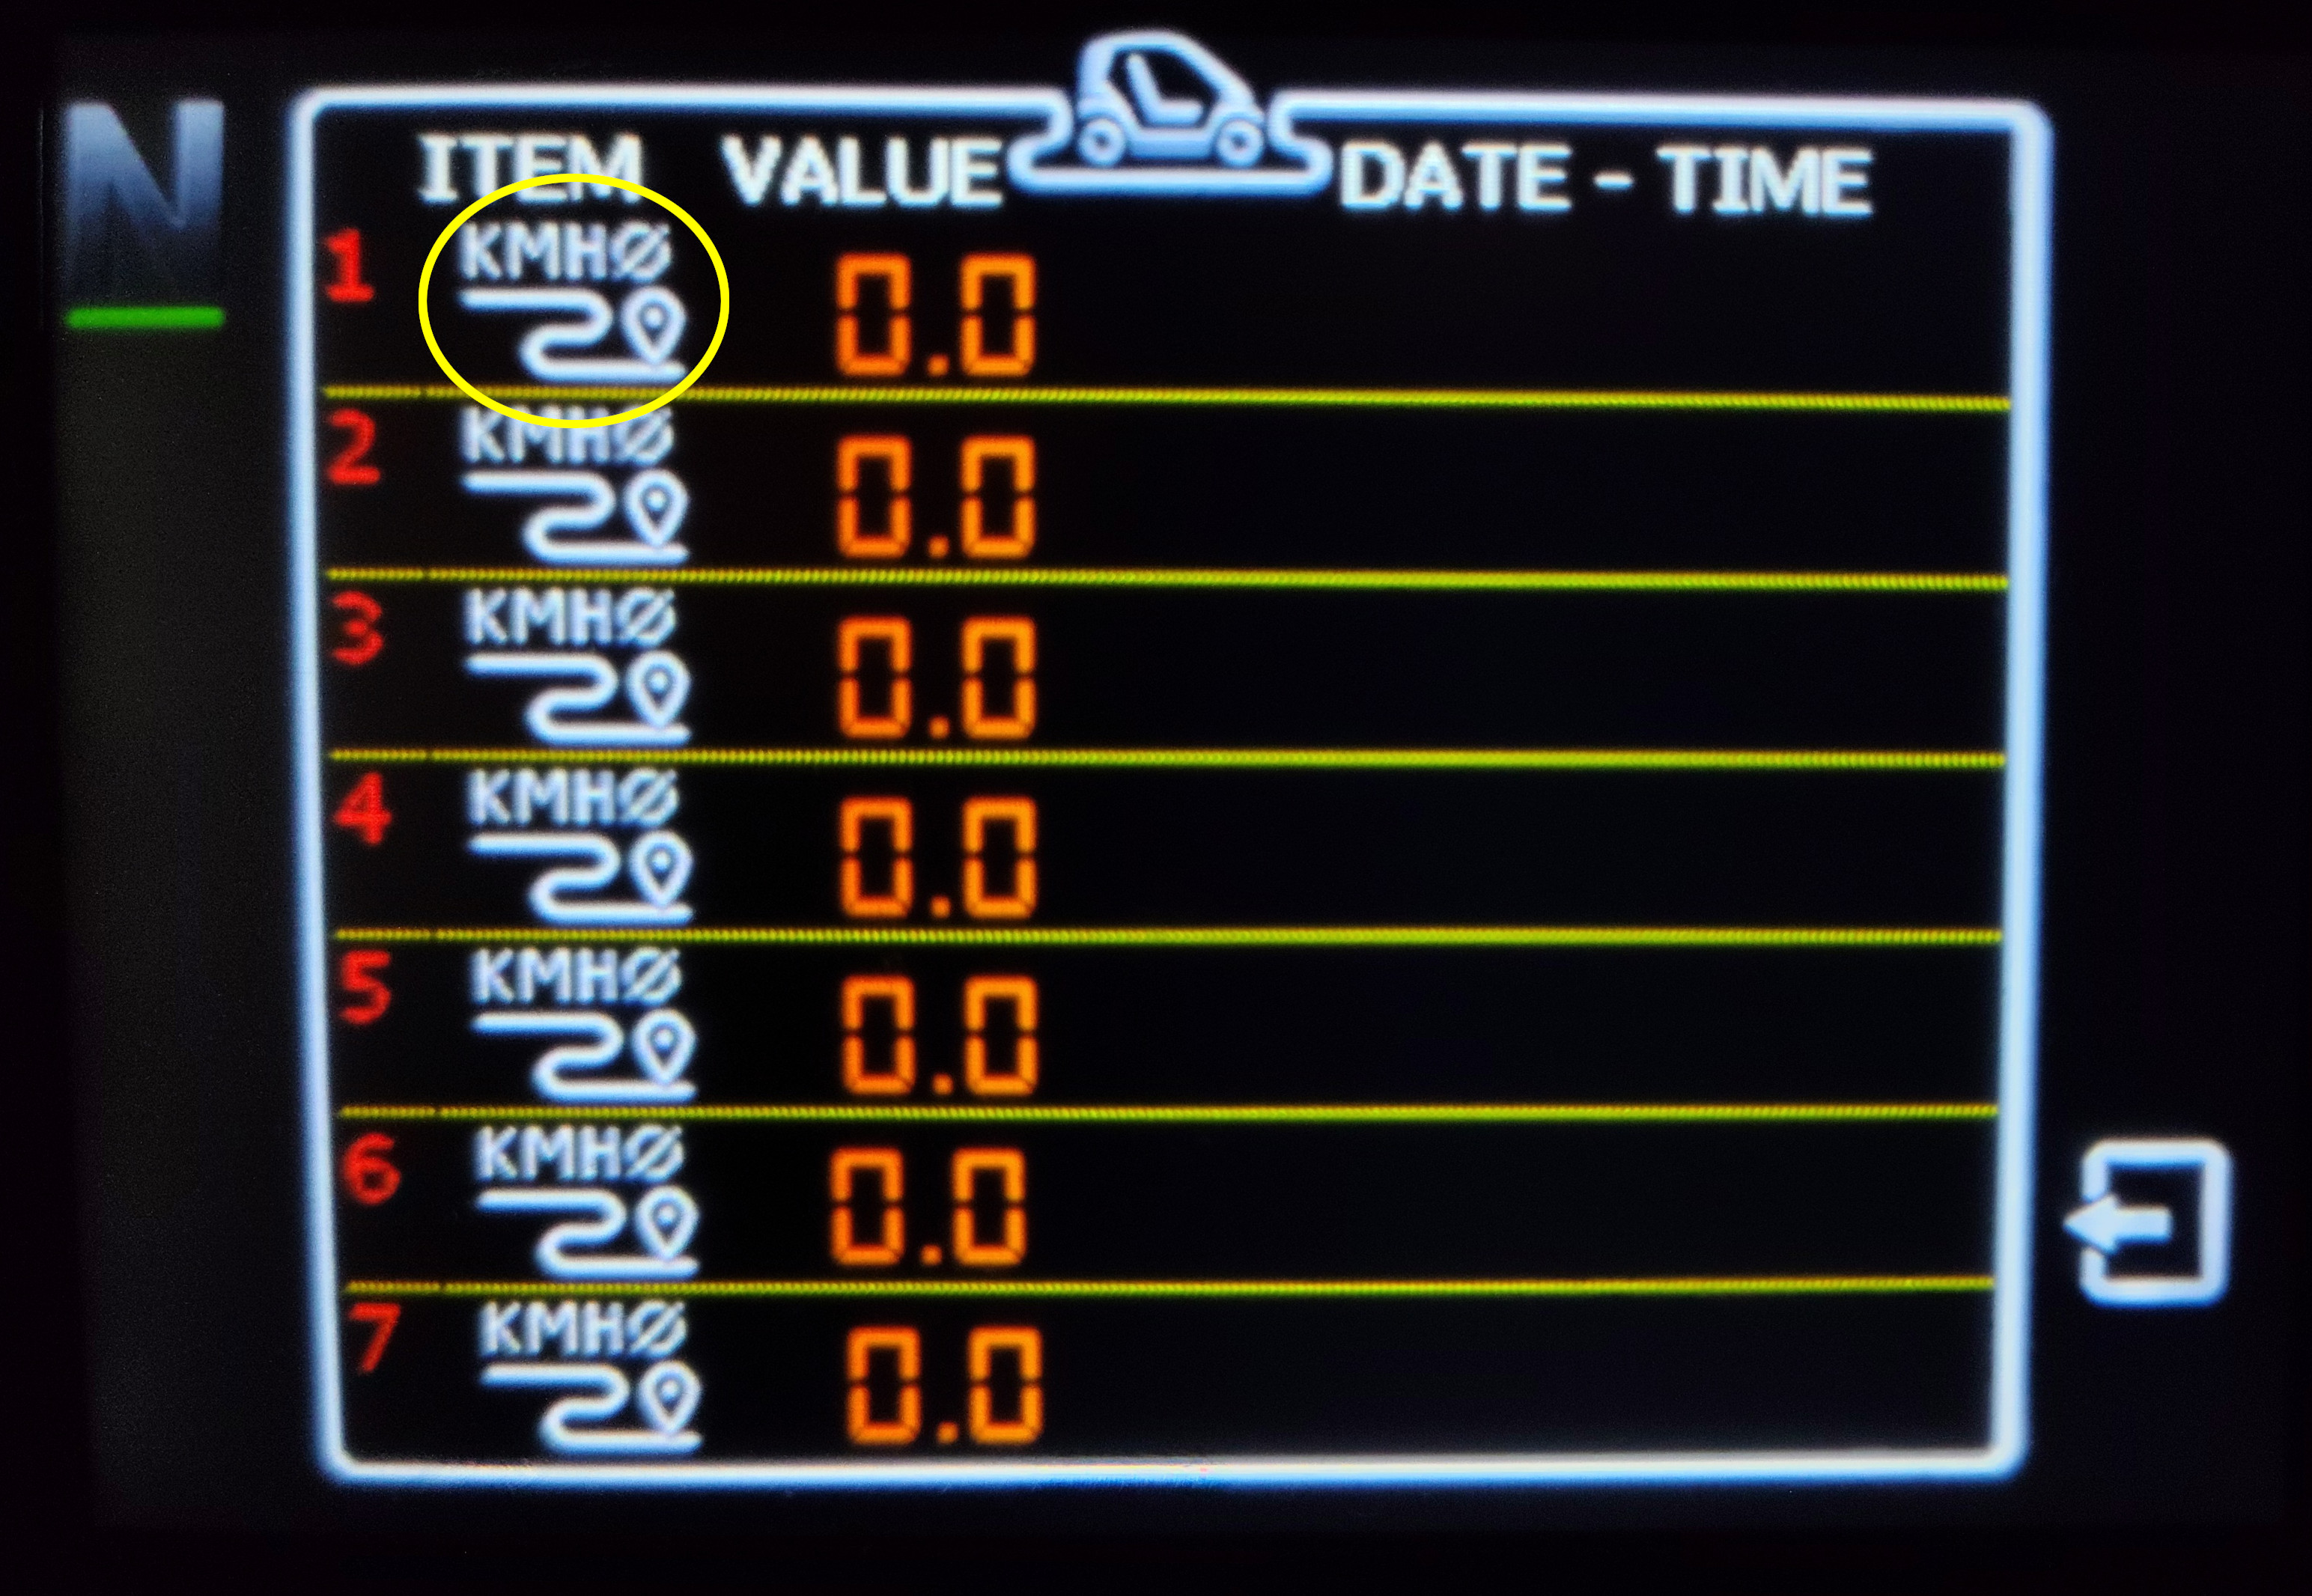
\includegraphics[width=\linewidth]{figures/trip_log_kmh.jpg}
        \caption{Affichage de la vitesse moyenne du trajet.}
    \end{subfigure}
\end{figure}

Sur le serveur web, vous pouvez les consulter toutes en même temps ; cela sera abordé dans la Section~\ref{sec:web_trip_history}.

\clearpage

\section{La page d'erreur}
\label{sec:error_page}

Cette page est similaire à la page du journal des alarmes et à la page d'historique des trajets, mais elle vous affichera les dernières erreurs DTC survenues. Les commandes permettant de supprimer des enregistrements ou de consulter les plus anciens ont déjà été abordées dans la Section~\ref{sec:alarm_log}.

\subsection{Comment accéder à la page d'erreur}

Cette page n'est pas accessible depuis la page principale, mais vous pouvez y accéder en \textbf{appuyant longuement sur l'icône du journal des alarmes} dans la ligne inférieure de l'écran jusqu'à ce qu'elle change. Comme nous l'avons vu précédemment, la séquence des pages disponibles par appui long sur l'icône du journal des alarmes est la suivante : page du journal des alarmes (Section~\ref{sec:alarm_log}) $\rightarrow$ page d'erreur $\rightarrow$ page de l'historique des trajets (Section~\ref{sec:trip_history}) $\rightarrow$ retour à la page du journal des alarmes, chacune avec son icône respective.\\

\begin{figure}[ht]
    \centering

    \begin{subfigure}[t]{0.48\textwidth}
        \centering
        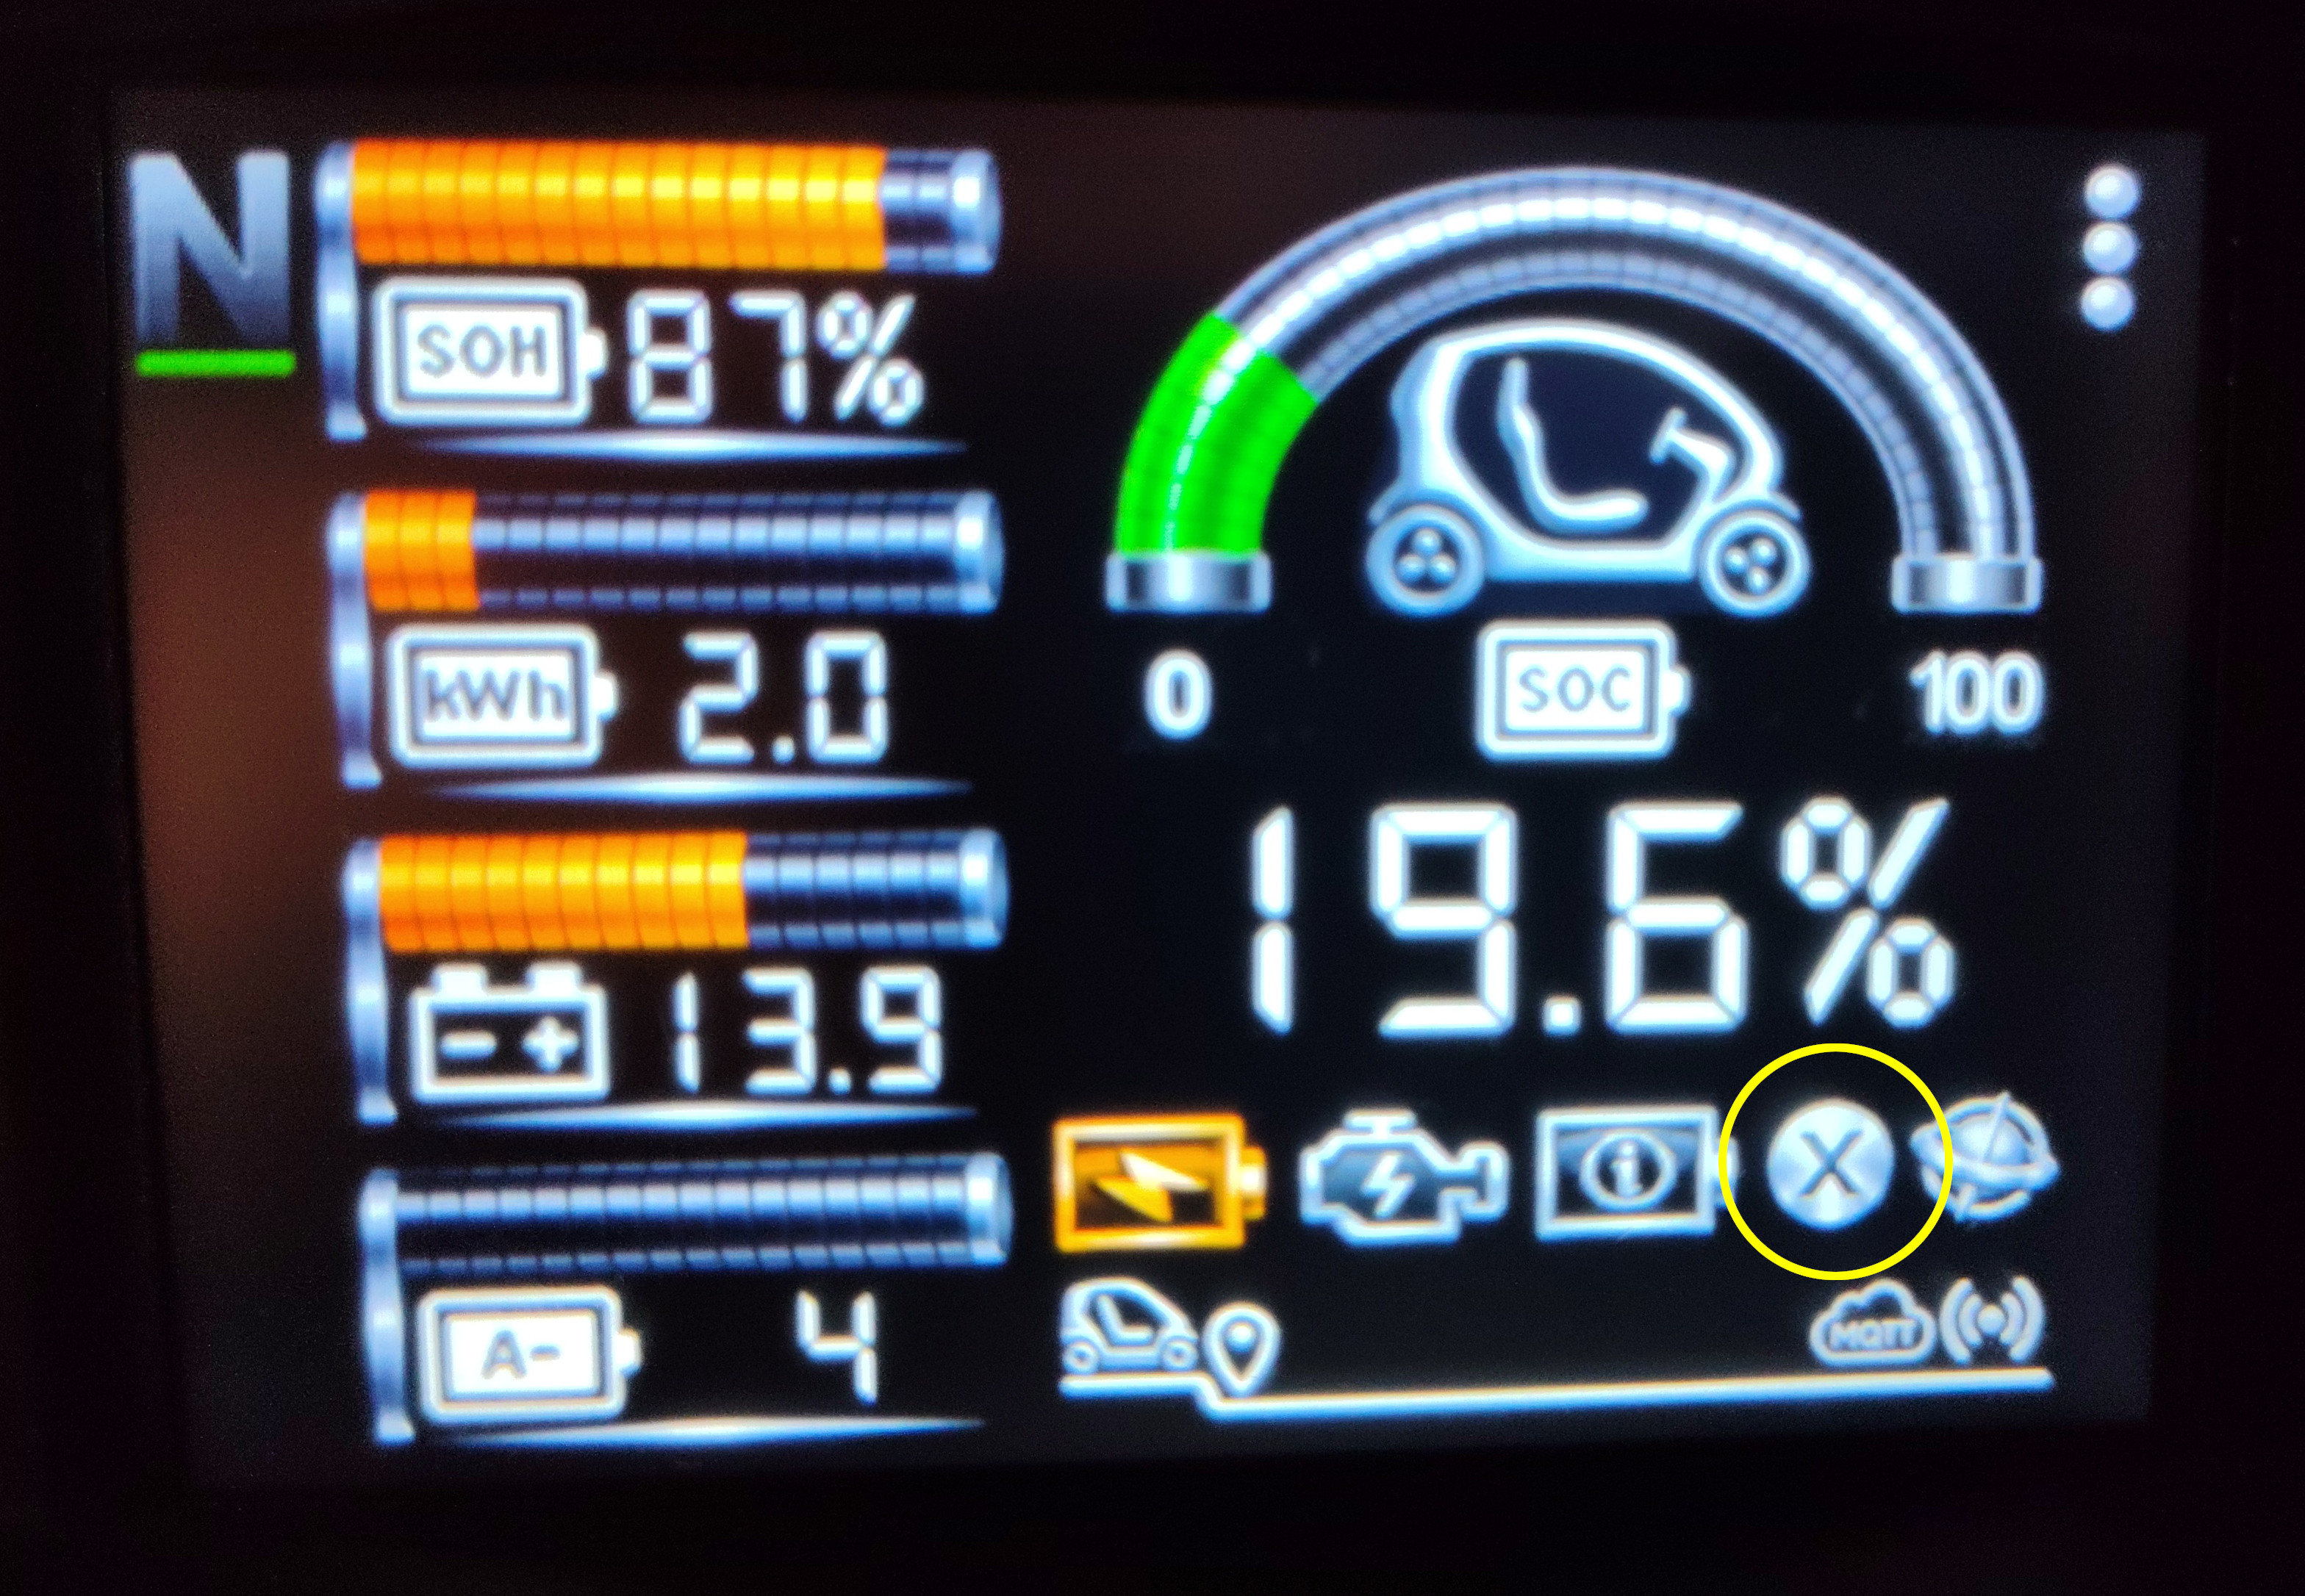
\includegraphics[width=\linewidth]{figures/enter_error_page.jpg}
        \caption{L'icône pour accéder à la page d'erreur.}
    \end{subfigure}
    \hfill
    \begin{subfigure}[t]{0.48\textwidth}
        \centering
        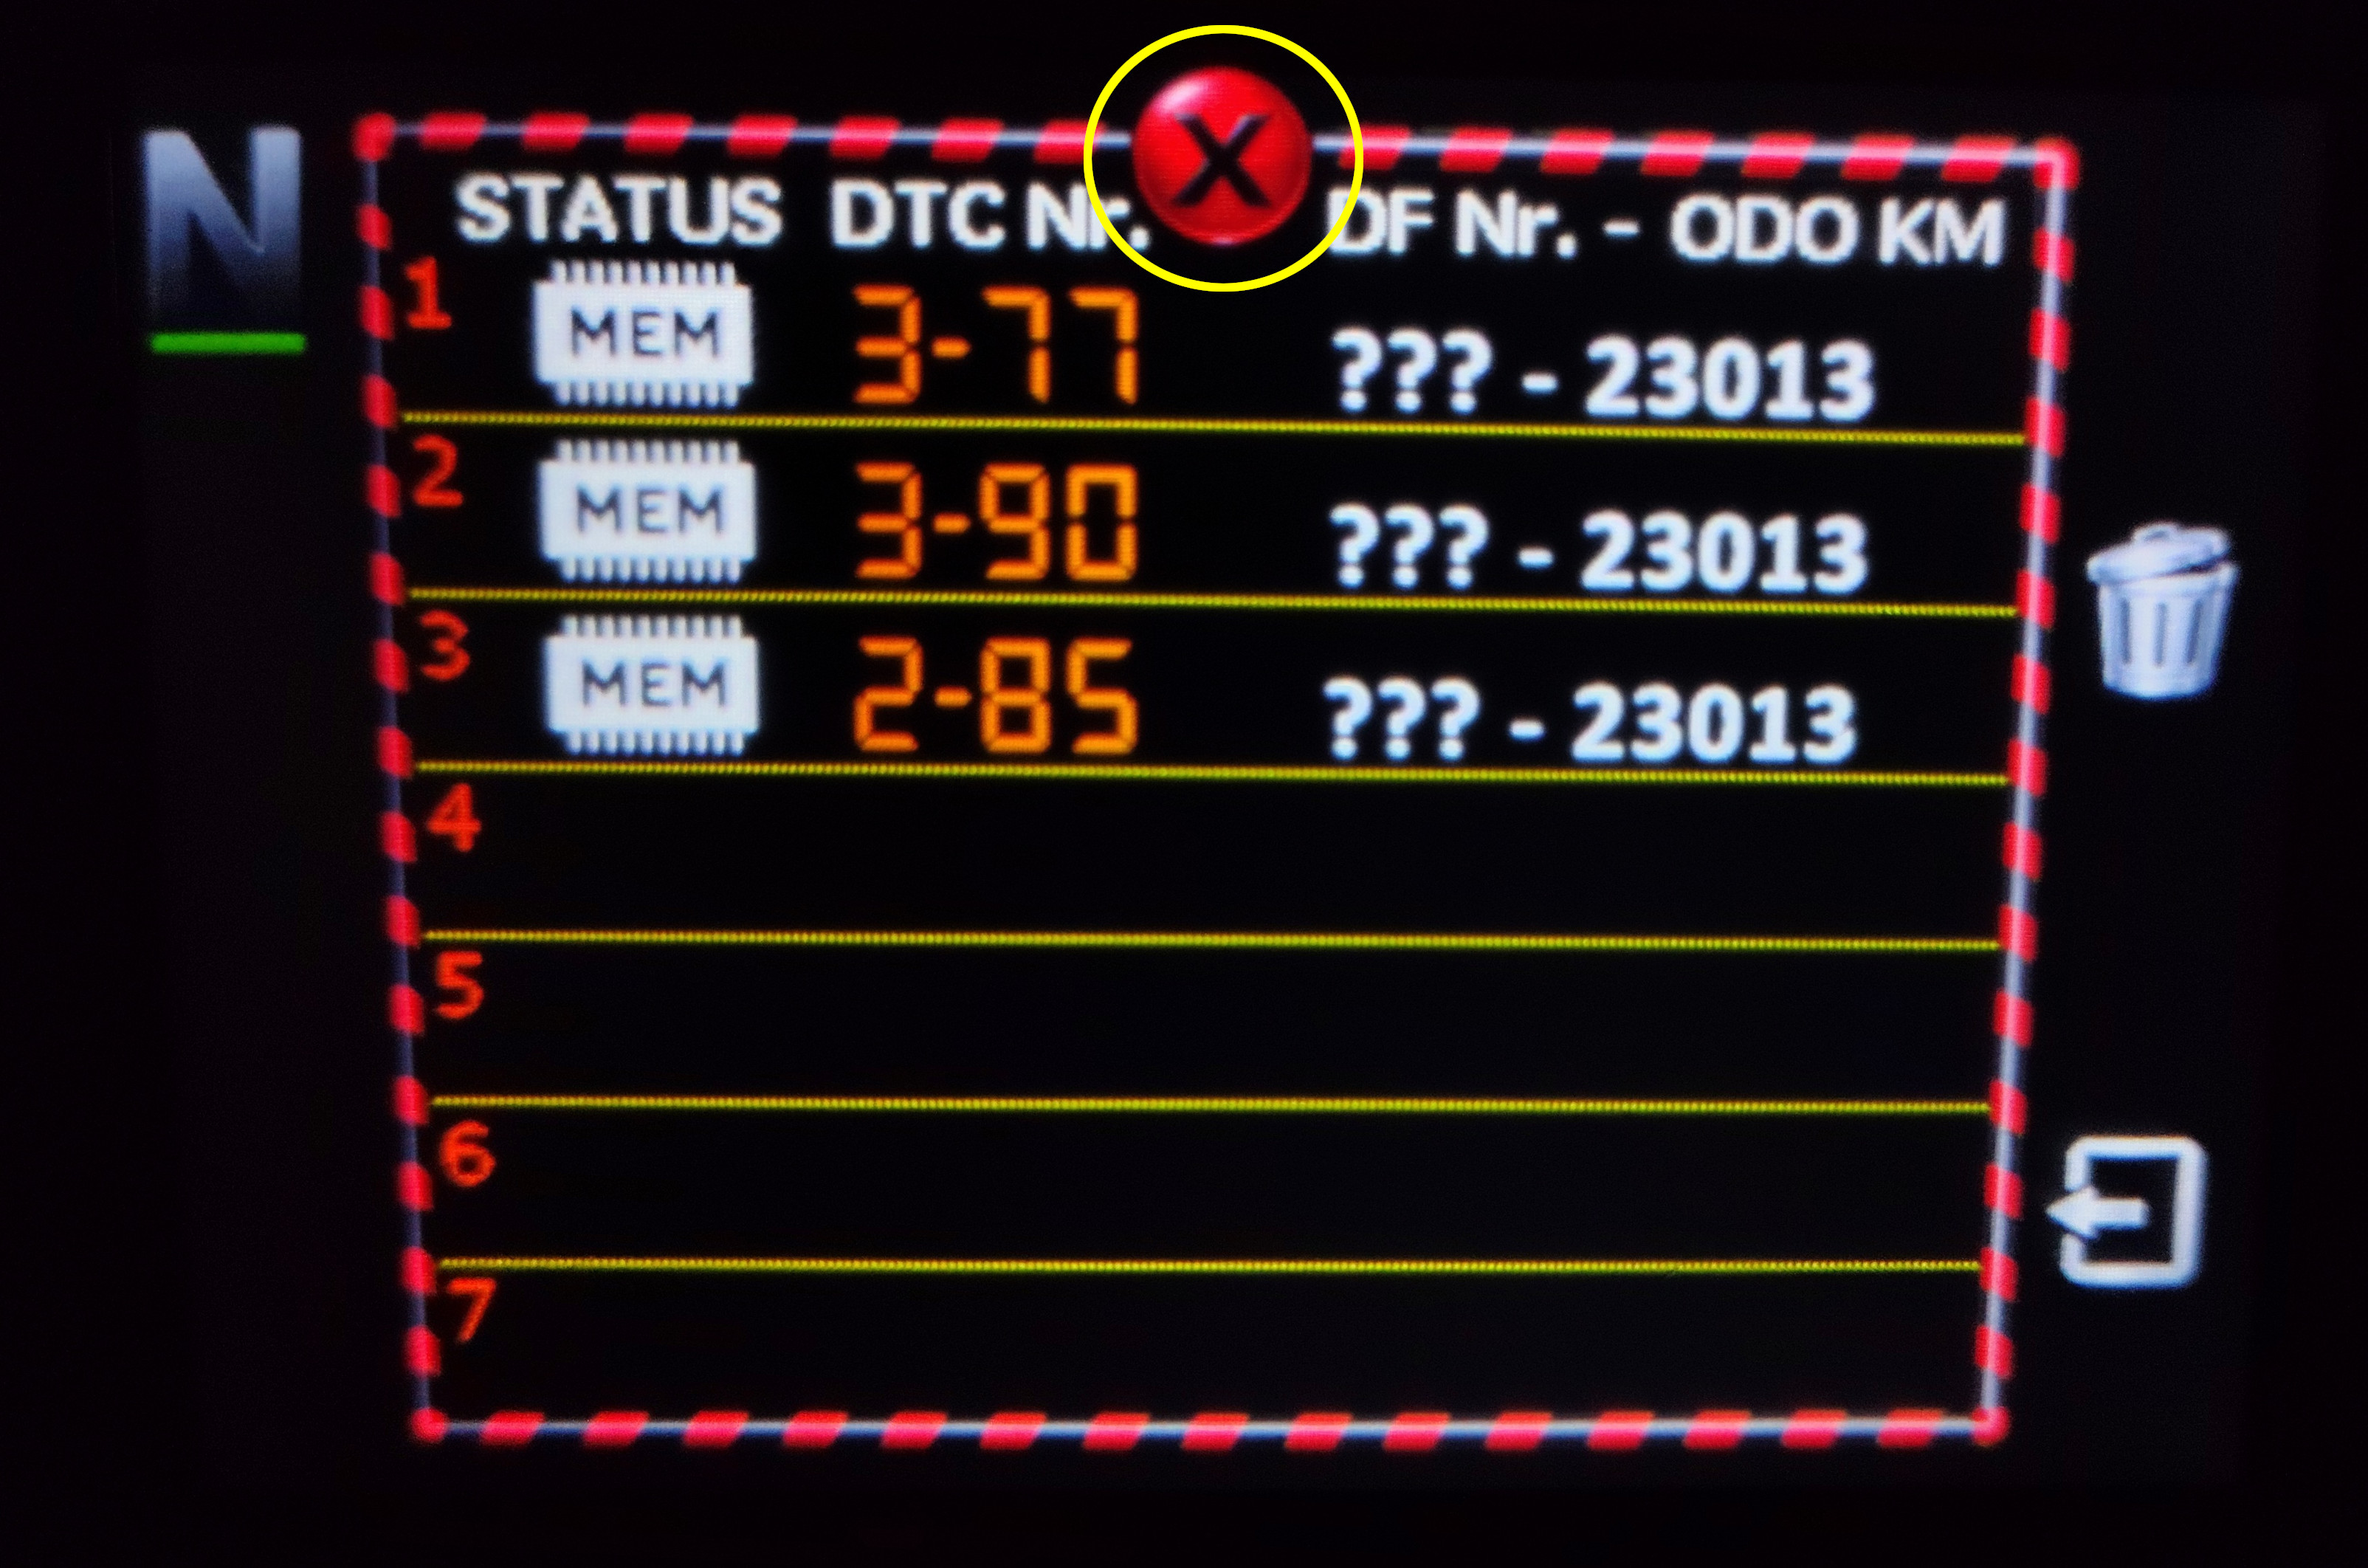
\includegraphics[width=\linewidth]{figures/error_page.jpg}
        \caption{Affichage de la page d'erreur.}
    \end{subfigure}
\end{figure}

\subsection{Commandes principales de la page d'erreur}

Comme vous pouvez le voir sur la deuxième image ci-dessus, la page d'erreur est similaire à la page du journal des alarmes. Elle affiche une liste des 14 dernières erreurs survenues, avec leur ODO, le numéro DTC, le numéro DF s'il est disponible, et une icône représentative. Reportez-vous à la page correspondante sur le serveur web pour plus d'informations telles que le SOC, la vitesse et une brève description (Section~\ref{sec:web_diagnostic}).\\

En appuyant sur l'icône de l'erreur (entourée en jaune sur l'image), vous pouvez faire défiler les pages des erreurs enregistrées, qui sont au nombre de 14 au total. La première page affiche les 7 dernières erreurs, tandis que la seconde affiche les plus anciennes. Pour \textbf{supprimer les enregistrements d'erreurs} à la fois sur cette page et sur la voiture, cliquez simplement sur l'icône de corbeille.\\

Comme sur d'autres pages, l'espace n'était pas suffisant pour placer les boutons de changement de page, vous pouvez donc appuyer sur le bouton de sortie dans le coin inférieur droit pour revenir à la page précédente, puis modifier la page active si vous le souhaitez.

\clearpage

\section{La page de recharge}
\label{sec:charging_page}

Cette page ne s'affiche pas en conduisant et il n'y a pas de bouton spécifique pour la visualiser. Cela est principalement dû au fait que cet écran de recharge apparaît automatiquement lorsque la Twizy est actuellement en cours de charge.

Comme vous pouvez le voir sur l'image, la disposition est la même que celle de la page du tableau de bord. Le SOC actuel est affiché au centre, remplaçant la valeur de la vitesse.\\

Une animation démarrera également, avec une vitesse différente selon le niveau de puissance de charge. Sur la photo ci-dessous se trouvent également des données spécifiques à la recharge, que vous pouvez modifier dans les paramètres comme expliqué ultérieurement. Sur cette page, vous n'avez pas la barre d'icônes d'état, mais vous disposez toujours des icônes d'état du réseau dans le coin inférieur droit, puisque vous pouvez également surveiller les valeurs de recharge de votre voiture lorsqu'elle est éteinte. En effet, ToM+ s'allumera automatiquement lorsque vous brancherez votre Twizy sur une source d'alimentation valide.

\begin{figure}[H]
    \centering
    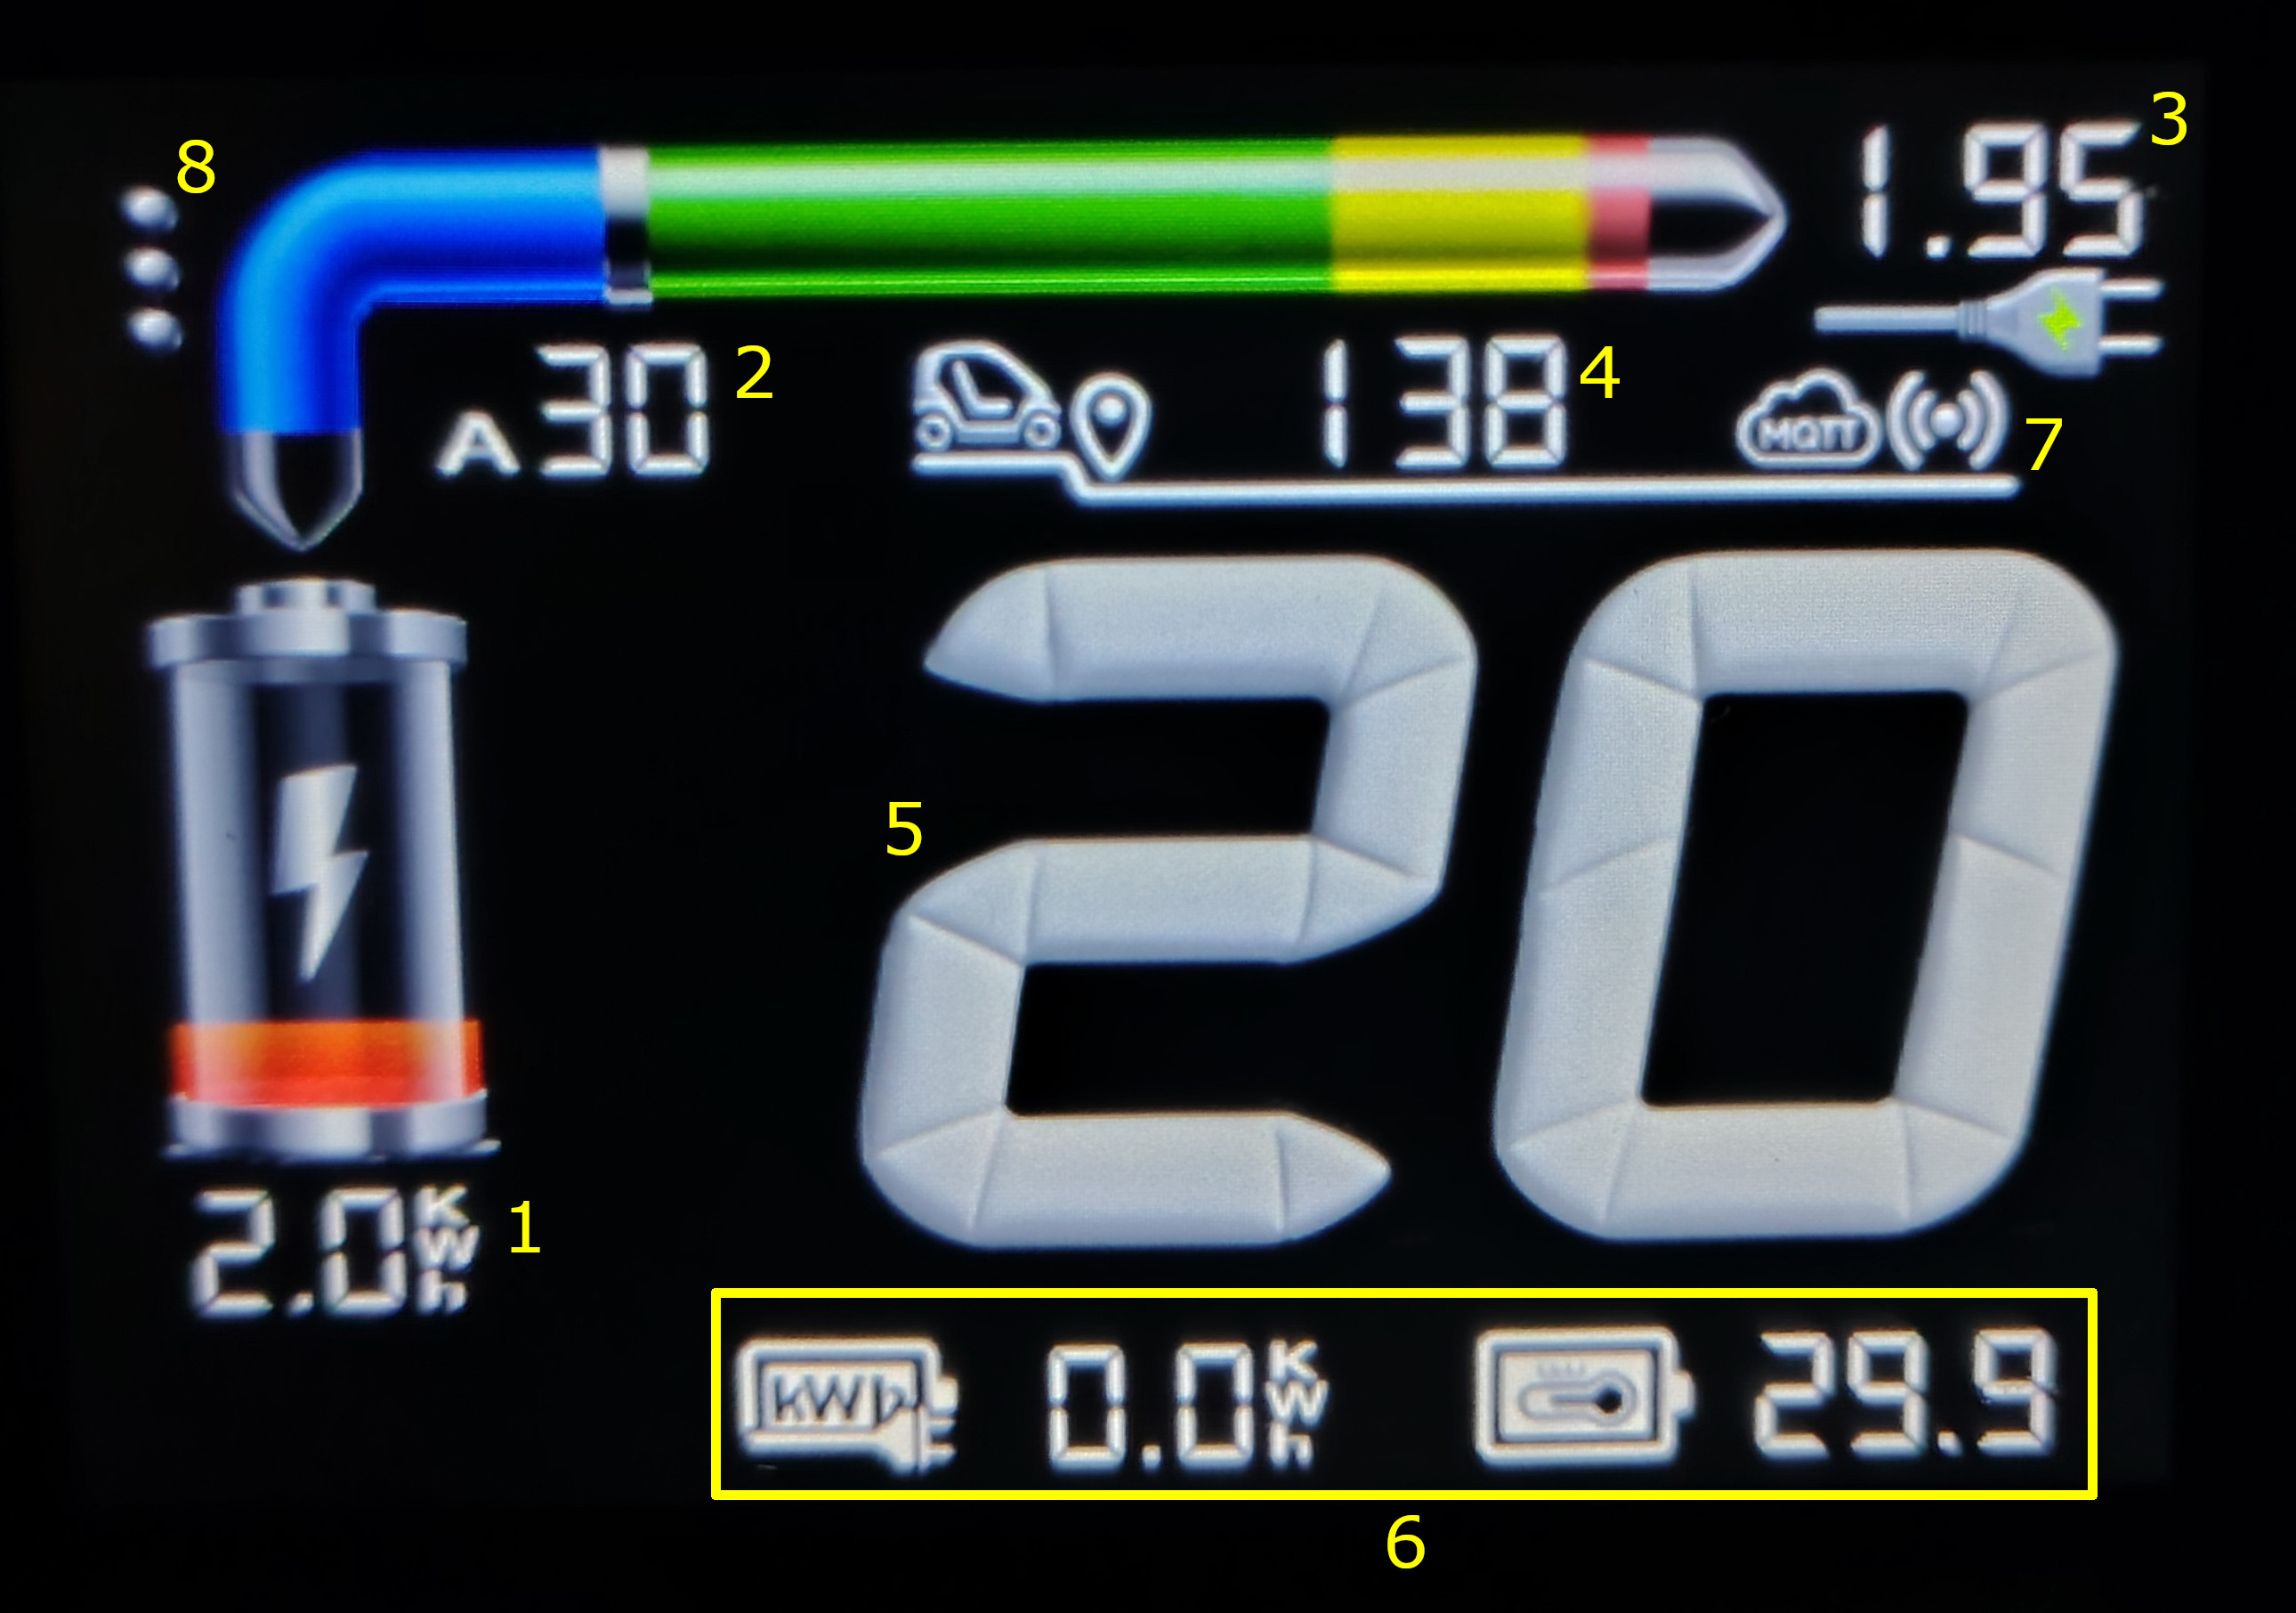
\includegraphics[width=0.8\textwidth]{figures/charging_page.jpg}
    \caption{La page de recharge.}
\end{figure}

\begin{description}
\item[\textbf{1}] Puissance actuelle stockée dans la batterie, exprimée en \(kWh\).
\item[\textbf{2}] Une valeur choisie entre le couple, la consommation d'énergie et la consommation de courant, qui est utilisée pour remplir la partie bleue de la barre de puissance. Appuyez sur la valeur pour faire défiler les trois options.
\item[\textbf{3}] Puissance de charge actuelle, exprimée en \(kW\), utilisée pour remplir le côté droit de la barre de puissance.
\item[\textbf{4}] Affiche l'ETA, c'est-à-dire le temps estimé pour terminer la charge.
\item[\textbf{5}] Le SOC actuel, c'est-à-dire l'état de charge de la batterie, exprimé en \%.
\item[\textbf{6}] Valeurs affichées supplémentaires, vous pouvez naviguer entre elles en appuyant sur l'icône pour modifier.
\item[\textbf{7}] Icônes pour MQTT et Wi-Fi. Grisées en cas de déconnexion, et colorées une fois connecté. Appuyez sur les icônes si vous souhaitez effectuer une nouvelle recherche Wi-Fi ou une reconnexion MQTT.
\item[\textbf{8}] Bouton de raccourci pour ouvrir la page des paramètres, afin d'accéder à des réglages plus avancés.
\end{description}

\section{La page des paramètres}
\label{sec:settings_page}

Afin de rendre ToM beaucoup plus personnalisable, voici la page des paramètres, accessible en appuyant sur les trois points dans le coin supérieur droit sur n'importe quelle page principale. Vous pouvez désormais facilement modifier l'apparence de base de votre ToM personnel.

\begin{figure}[H]
    \centering
    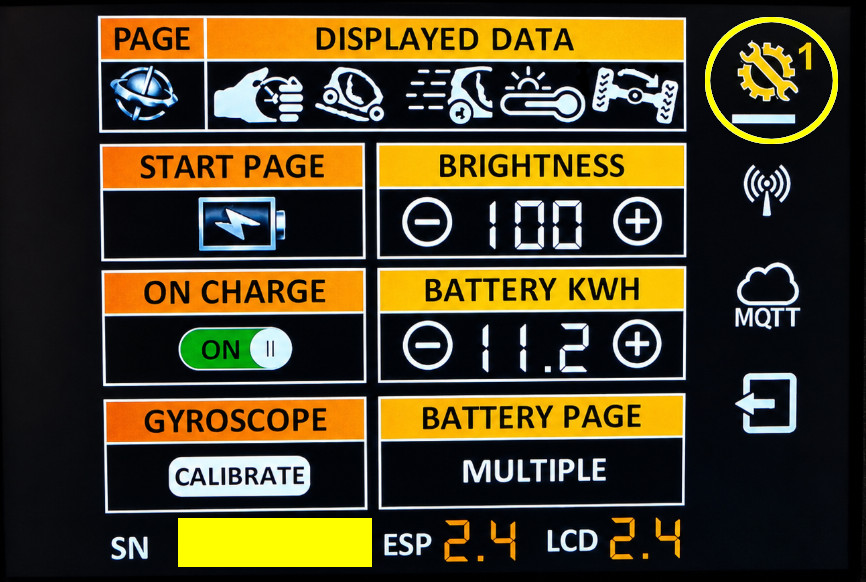
\includegraphics[width=0.8\textwidth]{figures/settings_page1.jpg}
    \caption{La première page des paramètres.}
    \label{fig:settings_page}
\end{figure}

\noindent La dernière ligne vous donnera des informations sur votre ToM personnel et affichera :
\begin{itemize}
    \item Le \textbf{numéro de série} de votre ToM dans le premier champ (censuré sur la figure ci-dessus)
    \item La version du microprogramme (firmware) du boîtier noir (ESP) (actuellement 2.4 sur la figure)
    \item La version du microprogramme (firmware) de l'écran tactile LCD (actuellement 2.4 sur la figure)
\end{itemize}
Vous pouvez effectuer la mise à jour vers la dernière version du microprogramme comme expliqué dans la Section~\ref{sec:update_procedure}.

\subsection{Première page des paramètres}

Comme vous pouvez le remarquer sur l'image ci-dessus, le bouton entouré dans le coin supérieur droit vous indiquera sur quelle page de paramètres vous vous trouvez actuellement. Dans ce cas, il s'agit de la première, mais vous pouvez appuyer dessus pour passer à la seconde. La première page concerne principalement l'apparence du ToM+, tandis que la seconde concerne le comportement du ToM+ et d'autres paramètres avancés.

\subsubsection{Personnalisation des valeurs de page}

Si vous souhaitez modifier l'ordre des données affichées dans l'une des pages ou même combiner des données provenant de différentes pages, vous pouvez le faire dans la page des paramètres, en suivant ces étapes.

\begin{figure}[H]
    \centering
    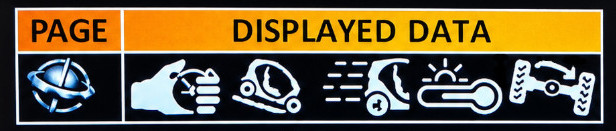
\includegraphics[width=0.8\textwidth]{figures/settings_page1_values.jpg}
    \caption{Personnalisation des valeurs de page.}
\end{figure}

En appuyant sur la première icône, vous ferez défiler toutes les pages disponibles dont les icônes ont été expliquées précédemment dans la Section~\ref{sec:page_icon_list} et qui vous permettront de personnaliser les valeurs pour cette page spécifique. Dans l'image ci-dessus, l'utilisateur a sélectionné la page gyroscope, donc les valeurs affichées à droite sont celles actuellement définies pour cette page.\\

Chacune des cinq icônes sous l'en-tête \textbf{Displayed Data} (Données affichées) peut être personnalisée simplement en appuyant dessus, en faisant défiler toutes les données jusqu'à trouver celle souhaitée (signification des icônes expliquée dans la Section~\ref{sec:icon_list}). Par exemple, vous pouvez également choisir de placer des données moteur sur la page batterie, combinant ainsi les deux.\\

\begin{figure}[H]
    \centering
    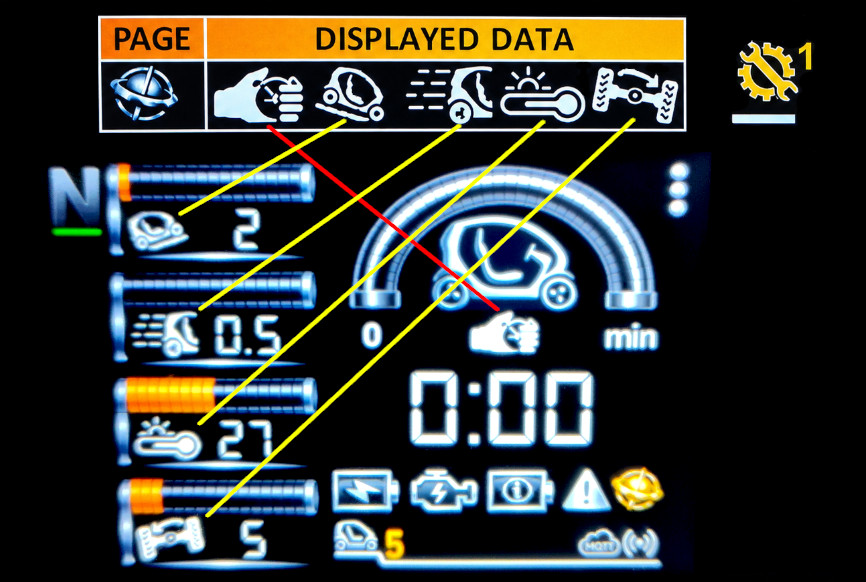
\includegraphics[width=0.8\textwidth]{figures/settings_page1_matching.jpg}
    \caption{Valeurs de disposition résultantes.}
    \label{fig:icon_arrangement}
\end{figure}

Après avoir personnalisé les valeurs affichées, \textbf{n'oubliez pas de sauvegarder en appuyant sur le bouton de sortie}. La nouvelle configuration apparaîtra comme indiqué sur la figure : la première donnée sera celle affichée au premier plan au centre de la page, tandis que toutes les autres seront répertoriées dans le tableau du côté gauche dans l'ordre que vous avez spécifié dans la page des paramètres.

\subsubsection{Choix de la page de démarrage}

Vous pouvez choisir quelle page sera la première à s'afficher lorsque vous quittez la page du tableau de bord. Pour ce faire, appuyez sur l'icône pour faire défiler toutes les pages disponibles jusqu'à trouver celle que vous souhaitez.

Dans l'image ci-dessous, l'utilisateur a sélectionné la page batterie, donc en quittant la page du tableau de bord, ToM+ l'affichera en premier.\\

\begin{figure}[H]
    \centering
    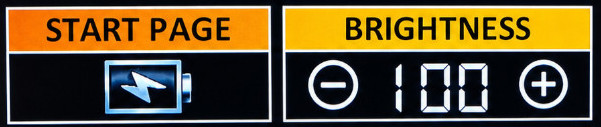
\includegraphics[width=0.8\textwidth]{figures/settings_page1_bright.jpg}
    \caption{Personnalisation de la page de démarrage et de la luminosité.}
\end{figure}

\subsubsection{Réglage de la luminosité de l'écran}

Comme vous pouvez le voir sur l'image ci-dessus, vous pouvez régler la luminosité de l'écran en appuyant sur les boutons \texttt{-} ou \texttt{+}. La luminosité peut être réglée de 0 à 100\% et la modification sera appliquée immédiatement.\\

\subsubsection{Activer/Désactiver la page de recharge}

ToM+ dispose d'une page spécifique pour afficher des données de charge plus détaillées (Section~\ref{sec:charging_page}). Vous pouvez choisir de la maintenir activée (\textit{croyez-moi, cela en vaut la peine !}) ou désactivée.

Appuyez ou faites glisser le bouton vers la gauche pour choisir entre ON et OFF. Lorsque le bouton glissant est réglé sur ON, le ToM démarre et charge la page de recharge lorsque votre Twizy est en charge ; sinon, à l'état OFF, il reste éteint pendant la charge. Pour enregistrer vos modifications, appuyez sur le bouton de sortie dans le coin inférieur droit.\\

\begin{figure}[H]
    \centering
    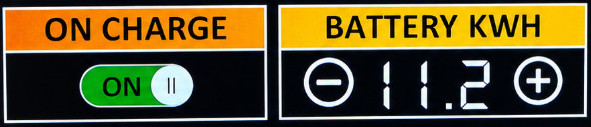
\includegraphics[width=0.8\textwidth]{figures/settings_page1_charge.jpg}
    \caption{Personnalisation de la page de recharge et des kWh de la batterie.}
\end{figure}

\subsubsection{Réglage de la capacité de votre batterie}

Vous pouvez définir la capacité de votre batterie en kWh, ce qui est utile si vous possédez une Twizy avec une batterie différente de celle d'origine. Cela aidera ToM+ à calculer l'autonomie restante de manière plus précise. Vous pouvez ajuster la valeur par pas de 0,1 kWh en appuyant sur les boutons \texttt{-} ou \texttt{+}, et le changement sera immédiatement appliqué. Veillez à \textbf{sauvegarder votre nouvelle configuration} en appuyant sur le bouton de sortie dans le coin inférieur droit.

\subsubsection{Calibrage du module gyroscope}

Si vous constatez que les données d'inclinaison du gyroscope pourraient être erronées, essayez d'appuyer sur le bouton « CALIBRATE » qui effectuera un calibrage du gyroscope. Assurez-vous d'être \textbf{sur une surface plane} avec votre Twizy avant d'effectuer cette opération, sinon vos données d'inclinaison risquent d'être encore pires. Le processus est illustré ci-dessous :

\begin{figure}[H]
    \centering
    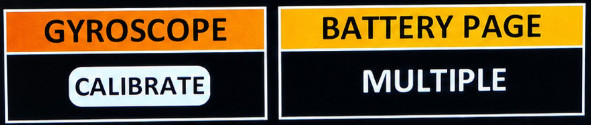
\includegraphics[width=0.8\textwidth]{figures/settings_page1_calibrate.jpg}
    \caption{Réglage du calibrage du gyroscope.}
\end{figure}

\subsubsection{Changement du mode de la page batterie}

Vous pouvez choisir d'avoir uniquement la page d'informations condensées de la batterie (Section~\ref{sec:condensed_binfo}) lorsque vous appuyez sur le bouton d'informations de la batterie ou non.

Les deux options disponibles sont \textit{'Condensed'} (Condensé) et \textit{'Multiple'} (Multiple) et vous pouvez basculer entre elles en appuyant sur le texte. La modification s'appliquera dès que vous appuyez sur le bouton de sortie dans le coin inférieur droit. Le mode \textbf{Multiple} affichera les quatre pages de batterie dont nous avons parlé dans la Section~\ref{sec:condensed_binfo}, tandis que le mode \textbf{Condensed} n'affichera que la page condensée.\\

\subsection{Seconde page des paramètres}

Cette seconde page de paramètres concerne certains réglages avancés sur le processus de recharge. Pour y accéder, appuyez sur le bouton entouré dans le coin supérieur droit de la première page de paramètres et appuyez à nouveau dessus pour revenir à la première page.\\

\begin{figure}[H]
    \centering
    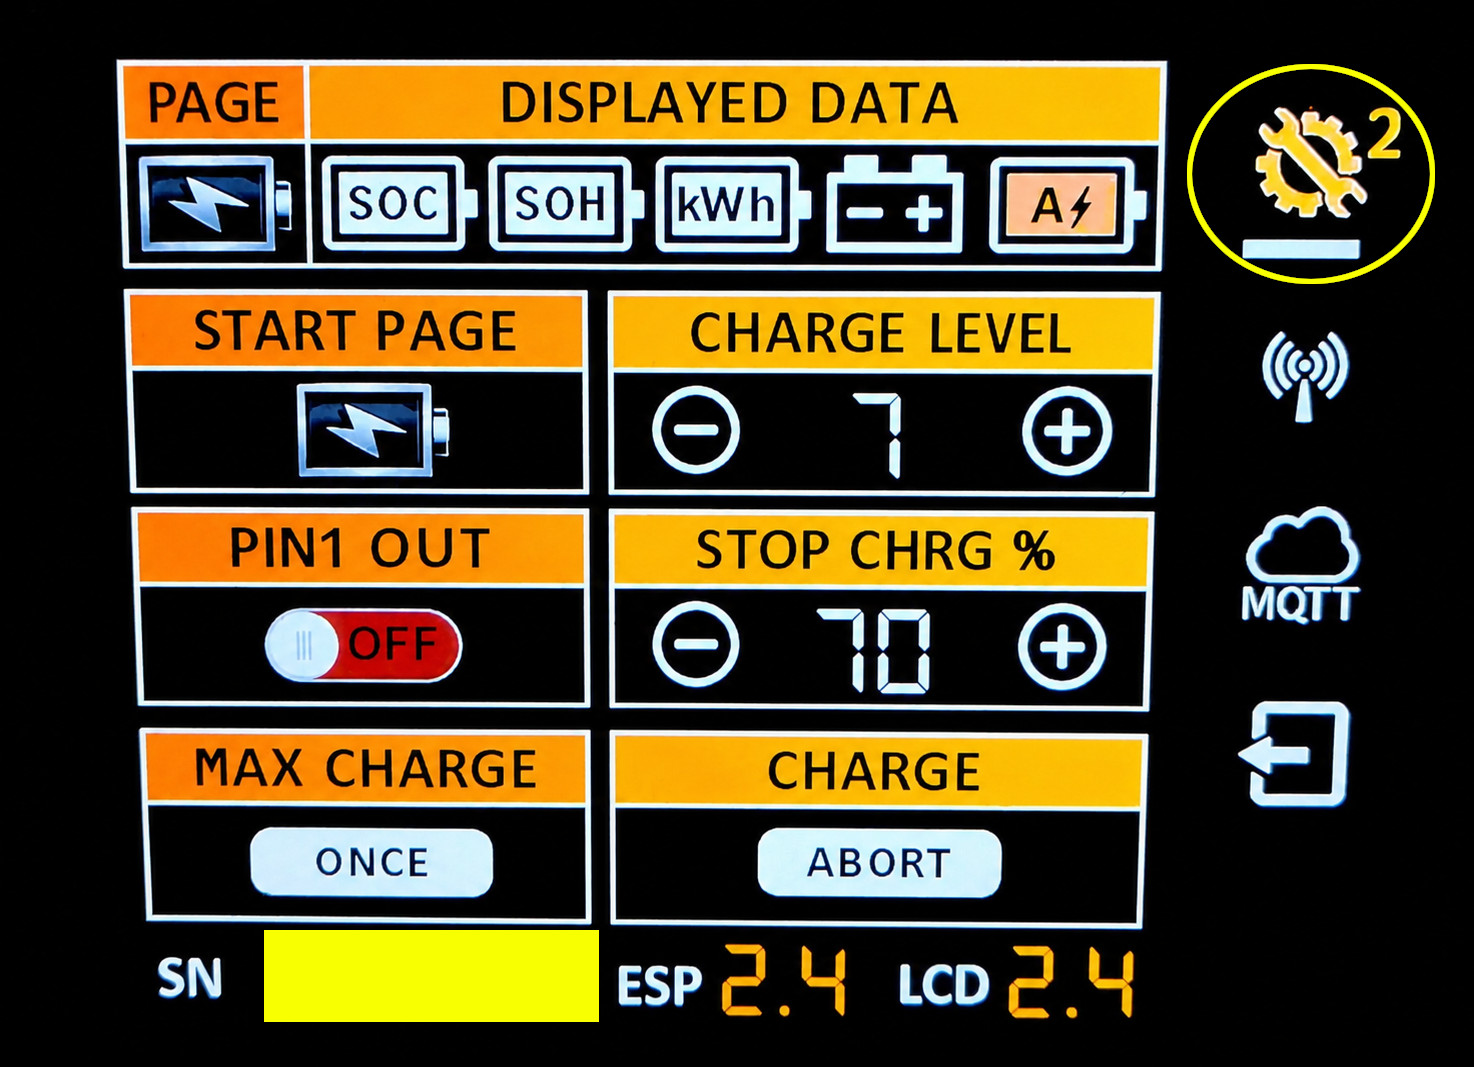
\includegraphics[width=0.8\textwidth]{figures/settings_page2.jpg}
    \caption{Seconde page des paramètres.}
\end{figure}

\subsubsection{Changement du niveau de charge}

Vous pouvez choisir le niveau de charge maximal de la batterie de votre Twizy, ce qui est utile si vous souhaitez limiter la puissance absorbée par la batterie pour augmenter sa durée de vie ou pour d'autres raisons. Le niveau \textit{'0'} signifie que le limiteur est désactivé, tandis que les niveaux \textit{'1'} à \textit{'7'} signifient l'utilisation du niveau de charge correspondant jusqu'au maximum disponible.

Pour augmenter ou diminuer le niveau, appuyez sur les boutons \texttt{-} ou \texttt{+}. La modification sera appliquée à la charge en cours si elle est déjà en cours, ou à la prochaine charge dans le cas contraire.\\

\begin{figure}[H]
    \centering
    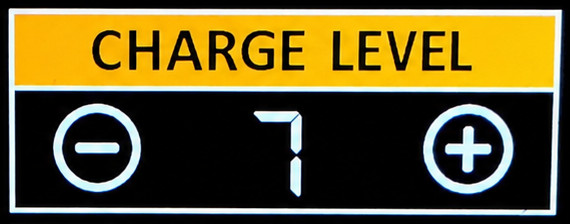
\includegraphics[width=0.6\textwidth]{figures/settings_page2_lvl.jpg}
    \caption{Changement du niveau de charge.}
\end{figure}

\subsubsection{Contrôle manuel de la broche PIN1 d'extension}

Certains utilisateurs ont signalé qu'il serait utile d'avoir un contrôle manuel de la broche PIN1 d'extension, normalement utilisée pour contrôler un chargeur auxiliaire. Ainsi, en cas de besoin, vous pouvez contrôler manuellement la broche PIN1 d'extension en appuyant sur le bouton ON/OFF. La modification sera appliquée dès que vous appuyez sur le bouton de sortie dans le coin inférieur droit.\\

\begin{figure}[H]
    \centering
    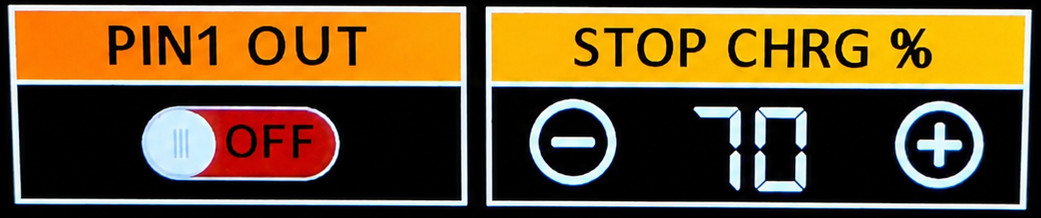
\includegraphics[width=0.8\textwidth]{figures/settings_page2_stop.jpg}
    \caption{Contrôle manuel de la broche PIN1 d'extension et arrêt du niveau de charge.}
\end{figure}

\subsubsection{Arrêt de la charge à un SOC spécifique}

Vous pouvez choisir d'arrêter la charge à un SOC spécifique, ce qui est utile si vous souhaitez augmenter la durée de vie de la batterie. Vous pouvez régler la valeur de 0 à 100\% en appuyant sur les boutons \texttt{-} ou \texttt{+}. La modification s'appliquera à la charge en cours si elle est déjà démarrée ou à la charge suivante dans le cas contraire.\\

\subsubsection{Effectuer une charge avec paramètres maximaux}

Vous pouvez choisir d'effectuer une charge sans limites de puissance et de SOC, ce qui est utile si vous souhaitez équilibrer les cellules de la batterie de temps en temps. Vous pouvez appuyer sur le bouton pour lancer la charge avec les paramètres maximaux, qui sera appliquée à la charge en cours ou à la charge suivante.\\

\begin{figure}[H]
    \centering
    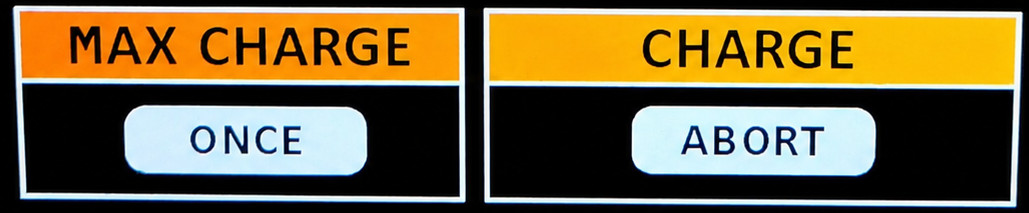
\includegraphics[width=0.8\textwidth]{figures/settings_page2_max.jpg}
    \caption{Charge avec paramètres maximaux et interruption du processus de charge.}
\end{figure}

\subsubsection{Interrompre le processus de charge}

Vous pouvez choisir d'interrompre le processus de recharge, ce qui est utile si vous souhaitez arrêter la charge immédiatement. Vous pouvez appuyer sur le bouton pour interrompre la charge, ce qui s'appliquera instantanément.\\

\clearpage

\subsection{Le menu du côté droit}

\iconbox{icons/SetupRed1.png}
{Page des paramètres (1 ou 2)}
{Indique sur quelle page de paramètres vous vous trouvez. Cliquez pour basculer.}

\iconbox{icons/WifiBianco.PNG}
{Page des paramètres Wi-Fi}
{Passe à la page des paramètres Wi-Fi. (Section~\ref{sec:wifi_settings})}

\iconbox{icons/MQTTBianco.PNG}
{Page des paramètres MQTT}
{Passe à la page des paramètres MQTT. (Section~\ref{sec:MQTT})}

\iconbox{icons/ExitIcon2.png}
{Bouton Enregistrer et Quitter}
{Enregistre les modifications et revient à la dernière page.}
